% Created 2024-05-11 Sat 14:46
% Intended LaTeX compiler: pdflatex
\documentclass[12pt]{article}

%%%% settings when exporting code %%%% 

\usepackage{listings}
\lstdefinestyle{code-small}{
backgroundcolor=\color{white}, % background color for the code block
basicstyle=\ttfamily\small, % font used to display the code
commentstyle=\color[rgb]{0.5,0,0.5}, % color used to display comments in the code
keywordstyle=\color{black}, % color used to highlight certain words in the code
numberstyle=\ttfamily\tiny\color{gray}, % color used to display the line numbers
rulecolor=\color{black}, % color of the frame
stringstyle=\color[rgb]{0,.5,0},  % color used to display strings in the code
breakatwhitespace=false, % sets if automatic breaks should only happen at whitespace
breaklines=true, % sets automatic line breaking
columns=fullflexible,
frame=single, % adds a frame around the code (non,leftline,topline,bottomline,lines,single,shadowbox)
keepspaces=true, % % keeps spaces in text, useful for keeping indentation of code
literate={~}{$\sim$}{1}, % symbol properly display via latex
numbers=none, % where to put the line-numbers; possible values are (none, left, right)
numbersep=10pt, % how far the line-numbers are from the code
showspaces=false,
showstringspaces=false,
stepnumber=1, % the step between two line-numbers. If it's 1, each line will be numbered
tabsize=1,
xleftmargin=0cm,
emph={anova,apply,class,coef,colnames,colNames,colSums,dim,dcast,for,ggplot,head,if,ifelse,is.na,lapply,list.files,library,logLik,melt,plot,require,rowSums,sapply,setcolorder,setkey,str,summary,tapply},
aboveskip = \medskipamount, % define the space above displayed listings.
belowskip = \medskipamount, % define the space above displayed listings.
lineskip = 0pt} % specifies additional space between lines in listings
\lstset{style=code-small}
%%%% packages %%%%%

\usepackage[utf8]{inputenc}
\usepackage[T1]{fontenc}
\usepackage{lmodern}
\usepackage{textcomp}
\usepackage{color}
\usepackage{graphicx}
\usepackage{grffile}
\usepackage{wrapfig}
\usepackage{rotating}
\usepackage{longtable}
\usepackage{multirow}
\usepackage{multicol}
\usepackage{changes}
\usepackage{pdflscape}
\usepackage{geometry}
\usepackage[normalem]{ulem}
\usepackage{amssymb}
\usepackage{amsmath}
\usepackage{amsfonts}
\usepackage{dsfont}
\usepackage{array}
\usepackage{ifthen}
\usepackage{hyperref}
\usepackage{natbib}
\RequirePackage{setspace} % to modify the space between lines - incompatible with footnote in beamer
\renewcommand{\baselinestretch}{1.1}
\geometry{a4paper, left=10mm, right=10mm, top=10mm}
\usepackage{titlesec}
\usepackage{etoolbox}

\makeatletter
\patchcmd{\ttlh@hang}{\parindent\z@}{\parindent\z@\leavevmode}{}{}
\patchcmd{\ttlh@hang}{\noindent}{}{}{}
\makeatother
\RequirePackage{colortbl} % arrayrulecolor to mix colors
\definecolor{myorange}{rgb}{1,0.2,0}
\definecolor{mypurple}{rgb}{0.7,0,8}
\definecolor{mycyan}{rgb}{0,0.6,0.6}
\newcommand{\lightblue}{blue!50!white}
\newcommand{\darkblue}{blue!80!black}
\newcommand{\darkgreen}{green!50!black}
\newcommand{\darkred}{red!50!black}
\definecolor{gray}{gray}{0.5}
\hypersetup{
citecolor=[rgb]{0,0.5,0},
urlcolor=[rgb]{0,0,0.5},
linkcolor=[rgb]{0,0,0.5},
}
\newenvironment{note}{\small \color{gray}\fontfamily{lmtt}\selectfont}{\par}
\newenvironment{activity}{\color{orange}\fontfamily{qzc}\selectfont}{\par}
\RequirePackage{pifont}
\RequirePackage{relsize}
\newcommand{\Cross}{{\raisebox{-0.5ex}%
{\relsize{1.5}\ding{56}}}\hspace{1pt} }
\newcommand{\Valid}{{\raisebox{-0.5ex}%
{\relsize{1.5}\ding{52}}}\hspace{1pt} }
\newcommand{\CrossR}{ \textcolor{red}{\Cross} }
\newcommand{\ValidV}{ \textcolor{green}{\Valid} }
\usepackage{stackengine}
\usepackage{scalerel}
\newcommand\Warning[1][3ex]{%
\renewcommand\stacktype{L}%
\scaleto{\stackon[1.3pt]{\color{red}$\triangle$}{\tiny\bfseries !}}{#1}%
\xspace
}
\RequirePackage{fancyvrb}
\DefineVerbatimEnvironment{verbatim}{Verbatim}{fontsize=\small,formatcom = {\color[rgb]{0.5,0,0}}}
\definecolor{grayR}{HTML}{8A8990}
\definecolor{grayL}{HTML}{C4C7C9}
\definecolor{blueM}{HTML}{1F63B5}
\newcommand{\Rlogo}[1][0.07]{
\begin{tikzpicture}[scale=#1]
\shade [right color=grayR,left color=grayL,shading angle=60]
(-3.55,0.3) .. controls (-3.55,1.75)
and (-1.9,2.7) .. (0,2.7) .. controls (2.05,2.7)
and (3.5,1.6) .. (3.5,0.3) .. controls (3.5,-1.2)
and (1.55,-2) .. (0,-2) .. controls (-2.3,-2)
and (-3.55,-0.75) .. cycle;

\fill[white]
(-2.15,0.2) .. controls (-2.15,1.2)
and (-0.7,1.8) .. (0.5,1.8) .. controls (2.2,1.8)
and (3.1,1.2) .. (3.1,0.2) .. controls (3.1,-0.75)
and (2.4,-1.45) .. (0.5,-1.45) .. controls (-1.1,-1.45)
and (-2.15,-0.7) .. cycle;

\fill[blueM]
(1.75,1.25) -- (-0.65,1.25) -- (-0.65,-2.75) -- (0.55,-2.75) -- (0.55,-1.15) --
(0.95,-1.15)  .. controls (1.15,-1.15)
and (1.5,-1.9) .. (1.9,-2.75) -- (3.25,-2.75)  .. controls (2.2,-1)
and (2.5,-1.2) .. (1.8,-0.95) .. controls (2.6,-0.9)
and (2.85,-0.35) .. (2.85,0.2) .. controls (2.85,0.7)
and (2.5,1.2) .. cycle;

\fill[white]  (1.4,0.4) -- (0.55,0.4) -- (0.55,-0.3) -- (1.4,-0.3).. controls (1.75,-0.3)
and (1.75,0.4) .. cycle;

\end{tikzpicture}
}
\RequirePackage{epstopdf} % to be able to convert .eps to .pdf image files
\RequirePackage{capt-of} %
\RequirePackage{caption} % newlines in graphics
\RequirePackage{tikz-cd} % graph
\RequirePackage{booktabs} % for nice lines in table (e.g. toprule, bottomrule, midrule, cmidrule)
\RequirePackage{amsmath}
\RequirePackage{algorithm}
\RequirePackage[noend]{algpseudocode}
\RequirePackage{dsfont}
\RequirePackage{amsmath,stmaryrd,graphicx}
\RequirePackage{prodint} % product integral symbol (\PRODI)
\usepackage{ifthen}
\usepackage{xifthen}
\usepackage{xargs}
\usepackage{xspace}
\newcommand\defOperator[7]{%
\ifthenelse{\isempty{#2}}{
\ifthenelse{\isempty{#1}}{#7{#3}#4}{#7{#3}#4 \left#5 #1 \right#6}
}{
\ifthenelse{\isempty{#1}}{#7{#3}#4_{#2}}{#7{#3}#4_{#1}\left#5 #2 \right#6}
}
}
\newcommand\defUOperator[5]{%
\ifthenelse{\isempty{#1}}{
#5\left#3 #2 \right#4
}{
\ifthenelse{\isempty{#2}}{\underset{#1}{\operatornamewithlimits{#5}}}{
\underset{#1}{\operatornamewithlimits{#5}}\left#3 #2 \right#4}
}
}
\newcommand{\defBoldVar}[2]{
\ifthenelse{\equal{#2}{T}}{\boldsymbol{#1}}{\mathbf{#1}}
}
\newcommandx\Esp[2][1=,2=]{\defOperator{#1}{#2}{E}{}{\lbrack}{\rbrack}{\mathbb}}
\newcommandx\Prob[2][1=,2=]{\defOperator{#1}{#2}{P}{}{\lbrack}{\rbrack}{\mathbb}}
\newcommandx\Qrob[2][1=,2=]{\defOperator{#1}{#2}{Q}{}{\lbrack}{\rbrack}{\mathbb}}
\newcommandx\Var[2][1=,2=]{\defOperator{#1}{#2}{V}{ar}{\lbrack}{\rbrack}{\mathbb}}
\newcommandx\Cov[2][1=,2=]{\defOperator{#1}{#2}{C}{ov}{\lbrack}{\rbrack}{\mathbb}}
\newcommandx\Binom[2][1=,2=]{\defOperator{#1}{#2}{B}{}{(}{)}{\mathcal}}
\newcommandx\Gaus[2][1=,2=]{\defOperator{#1}{#2}{N}{}{(}{)}{\mathcal}}
\newcommandx\Wishart[2][1=,2=]{\defOperator{#1}{#2}{W}{ishart}{(}{)}{\mathcal}}
\newcommandx\Likelihood[2][1=,2=]{\defOperator{#1}{#2}{L}{}{(}{)}{\mathcal}}
\newcommandx\logLikelihood[2][1=,2=]{\defOperator{#1}{#2}{\ell}{}{(}{)}{}}
\newcommandx\Information[2][1=,2=]{\defOperator{#1}{#2}{I}{}{(}{)}{\mathcal}}
\newcommandx\Hessian[2][1=,2=]{\defOperator{#1}{#2}{H}{}{(}{)}{\mathcal}}
\newcommandx\Score[2][1=,2=]{\defOperator{#1}{#2}{S}{}{(}{)}{\mathcal}}
\newcommandx\Vois[2][1=,2=]{\defOperator{#1}{#2}{V}{}{(}{)}{\mathcal}}
\newcommandx\IF[2][1=,2=]{\defOperator{#1}{#2}{IF}{}{(}{)}{\mathcal}}
\newcommandx\Ind[1][1=]{\defOperator{}{#1}{1}{}{(}{)}{\mathds}}
\newcommandx\Max[2][1=,2=]{\defUOperator{#1}{#2}{(}{)}{min}}
\newcommandx\Min[2][1=,2=]{\defUOperator{#1}{#2}{(}{)}{max}}
\newcommandx\argMax[2][1=,2=]{\defUOperator{#1}{#2}{(}{)}{argmax}}
\newcommandx\argMin[2][1=,2=]{\defUOperator{#1}{#2}{(}{)}{argmin}}
\newcommandx\cvD[2][1=D,2=n \rightarrow \infty]{\xrightarrow[#2]{#1}}
\newcommandx\Hypothesis[2][1=,2=]{
\ifthenelse{\isempty{#1}}{
\mathcal{H}
}{
\ifthenelse{\isempty{#2}}{
\mathcal{H}_{#1}
}{
\mathcal{H}^{(#2)}_{#1}
}
}
}
\newcommandx\dpartial[4][1=,2=,3=,4=\partial]{
\ifthenelse{\isempty{#3}}{
\frac{#4 #1}{#4 #2}
}{
\left.\frac{#4 #1}{#4 #2}\right\rvert_{#3}
}
}
\newcommandx\dTpartial[3][1=,2=,3=]{\dpartial[#1][#2][#3][d]}
\newcommandx\ddpartial[3][1=,2=,3=]{
\ifthenelse{\isempty{#3}}{
\frac{\partial^{2} #1}{\partial #2^2}
}{
\frac{\partial^2 #1}{\partial #2\partial #3}
}
}
\newcommand\Real{\mathbb{R}}
\newcommand\Rational{\mathbb{Q}}
\newcommand\Natural{\mathbb{N}}
\newcommand\trans[1]{{#1}^\intercal}%\newcommand\trans[1]{{\vphantom{#1}}^\top{#1}}
\newcommand{\independent}{\mathrel{\text{\scalebox{1.5}{$\perp\mkern-10mu\perp$}}}}
\newcommand\half{\frac{1}{2}}
\newcommand\normMax[1]{\left|\left|#1\right|\right|_{max}}
\newcommand\normTwo[1]{\left|\left|#1\right|\right|_{2}}
\newcommand\Veta{\boldsymbol{\eta}}
\newcommand{\Model}{\mathcal{M}}
\newcommand{\ModelHat}{\widehat{\mathcal{M}}}
\newcommand{\param}{\Theta}
\newcommand{\paramHat}{\widehat{\param}}
\newcommand{\paramCon}{\widetilde{\param}}
\newcommand{\Vparam}{\boldsymbol{\param}}
\newcommand{\VparamT}{\Vparam_0}
\newcommand{\VparamHat}{\boldsymbol{\paramHat}}
\newcommand{\VparamCon}{\boldsymbol{\paramCon}}
\newcommand{\X}{X}
\newcommand{\x}{x}
\newcommand{\VX}{\boldsymbol{X}}
\newcommand{\Vx}{\boldsymbol{x}}
\newcommand{\Y}{Y}
\newcommand{\y}{y}
\newcommand{\VY}{\boldsymbol{Y}}
\newcommand{\Vy}{\boldsymbol{y}}
\newcommand{\Vvarepsilon}{\boldsymbol{\varepsilon}}
\author{Brice Ozenne}
\date{\today}
\title{Overview of the package LMMstar}
\hypersetup{
 colorlinks=true,
 pdfauthor={Brice Ozenne},
 pdftitle={Overview of the package LMMstar},
 pdfkeywords={},
 pdfsubject={},
 pdfcreator={Emacs 27.1 (Org mode 9.4.6)},
 pdflang={English}
 }
\begin{document}

\maketitle
This vignette describes the main functionalities of the \textbf{LMMstar}
package. This package implements specific types of linear mixed
models, mainly useful when having repeated observations over a
discrete variable: \(\VY=(Y_1,\ldots,Y_T)\) where \(T\) can be
for example be time (chronological ordering of the repetitions) or
brain region (arbitrary ordering of the repetitions). Denoting by
\(\VX\) the associated covariates and \(\boldsymbol{\varepsilon} =
(\varepsilon_1,\ldots,\varepsilon_T)\), the model can be written:
\[ \VY = \VX \beta + \boldsymbol{\varepsilon} \text{ where } \varepsilon \sim \Gaus(0,\Omega) \]
where \(\beta\) are the mean parameters and the residual
variance-covariance matrix, \(\Omega\), depends on a set of
variance-covariance parameters (say \(\gamma\)) distinct of
\(\beta\). Key assumptions are:
\begin{itemize}
\item we observe \(n\) independent replicates of
\(\mathcal{O}=(\VY,\VX)\), i.e. at the cluster level,
observations \(\left(\mathcal{O}_1,\ldots,\mathcal{O}_n\right)\) are
independent. The replicates should also be identically distributed
up to a categorical variable (called strata variable in the following).
\item the residual variance is independent of the mean value.
\end{itemize}
Additional assumptions are necessary in presence of missing values,
typically correct specification of the conditional mean to have
consistent estimates of the mean parameters. This case will sometimes
be examplified by considering that only last outcome may be missing:
the conditional mean \(\Esp[Y_T|Y_1,Y_2,\ldots,Y_{T-1}]\) is then
abreviated as \(\Esp[Y_T|Y_{T-1}]\). Note that we do not require the
residuals to be normally distributed to have valid estimates or
statistical inference in large samples.

\bigskip

To get start, one should load the \textbf{LMMstar} package in the \Rlogo session:
\lstset{language=r,label= ,caption= ,captionpos=b,numbers=none}
\begin{lstlisting}
library(LMMstar)
\end{lstlisting}

This package is under active development. Newer package versions may
include additional functionalities and fix previous bugs. The version
of the package that is being used for this overview is:
\lstset{language=r,label= ,caption= ,captionpos=b,numbers=none}
\begin{lstlisting}
utils::packageVersion("LMMstar")
\end{lstlisting}

\begin{verbatim}
[1] '1.1.0'
\end{verbatim}


It is recommanded to also the following packages, as some of the
methods implemented in the package are relative to a generic method
implmented in other packages:
\lstset{language=r,label= ,caption= ,captionpos=b,numbers=none}
\begin{lstlisting}
library(ggplot2) ## autoplot method
library(nlme) ## ranef method
library(lava) ## iid, information, manifest methods
\end{lstlisting}

\clearpage

The user interface of the \textbf{LMMstar} package is made of the following
functions:
\begin{itemize}
\item functions to describe or visualize the dataset: 
\begin{itemize}
\item \texttt{scatterplot} to visualize the marginal and bivariate distribution of continuous variables.
\item \texttt{summarize} to compute summary statistics, possibly stratified on a categorical variable.
\item \texttt{summarizeNA} to identify missing data patterns.
\item \texttt{partialCor} to compute partial correlation between two variables.
\end{itemize}
\item the function \texttt{mt.test} to perform multiple Student's t-Tests and
adjust the results for multiple testing.
\item the function \texttt{lmm} is the main function of the package which fits
linear mixed models. The user can interact with \emph{lmm} objects using:
\begin{itemize}
\item \texttt{anova} to perform Wald tests, i.e. test linear combinations of
coefficients (\(\widehat{\beta}_1+\widehat{\beta}_2=0\) or
\(\widehat{\beta}_1=\widehat{\beta}_2=0\)). The output obtained
with different \texttt{lmm} can be combined using \texttt{rbind}.
\item \texttt{coef} to extract the estimated model parameters (\(\widehat{\beta}\) and possibly \(\widehat{\gamma}\)).
\item \texttt{confint} to extract the estimates with their confidence intervals.
\item \texttt{effects} to evaluate marginal effects, e.g. \(\Esp\left[\Esp[Y|X_1=1]-\Esp[Y|X_1=0]\right]\) when \(\VX=(X_1,X_2)\).
\item \texttt{estimate} to test non-linear combinations of coefficients (Wald test via a first order delta method, e.g. \(\widehat{\beta}_1/\widehat{\beta}_2=1\)).
\item \texttt{fitted} to output the fitted mean (\(X\widehat{\beta}\)) or the
conditional mean for observations with missing outcome
(e.g. \(X\widehat{\beta} +
      \widehat{\Esp}[\varepsilon_T|\varepsilon_{-T}]\)).
\item \texttt{iid} to extract the influence function of the estimated
parameters (\(\varphi\)), which satisfies \newline
\(\sqrt{n}(\widehat{\beta}-\beta) = \frac{1}{\sqrt{n}}
      \sum_{i=1}^n \varphi\left(\mathcal{O}_i\right) +o_p(1)\)
\item \texttt{levels} to extract the reference level for the mean structure.
(i.e. what \texttt{(Intercept)} refers to in presence of categorical.
covariates).
\item \texttt{logLik} to output the log-likelihood of the estimated model.
\item \texttt{model.tables} to extract the estimates, standard errors, p-value, and confidence intervals.
\item \texttt{plot} to obtain a diagnostic plots, partial residual plots, or a graphical display of the fitted values.
\item \texttt{predict} to compute the mean conditional on covariates and
possible outcome values.
\item \texttt{profile} to display the likelihood or profile likelihood of the model.
\item \texttt{resample} to use non-parametric bootstrap or permutation test for statistical inference.
\item \texttt{residuals} to extract the observed residuals of the fitted
model, possibly normalized
(\(\widehat{\Omega}^{-\frac{1}{2}}\widehat{\varepsilon}\)).
\item \texttt{sigma} to extract the modeled residual variance covariance matrix (\(\widehat{\Omega}\)).
\item \texttt{summary} to obtain a summary of the input, model fit, and estimated values.
\item \texttt{vcov} to extract the variance-covariance matrix of the mean
parameters (\(\widehat{\Sigma}_{\widehat{\beta}}\)).
\end{itemize}
\item the \texttt{mlmm} function to fit group-specific linear mixed models and
gather the estimated coefficients.
\item the \texttt{sampleRem} function to simulate longitudinal data.
\item the \texttt{LMMstar.options} function enables the user to display the
default values used in the \textbf{LMMstar} package. The function
can also change the default values to better match the user needs.
\end{itemize}


\clearpage

\section{Illustrative dataset}
\label{sec:org6b56c9d}

To illustrate the functionalities of the package, we will use the
gastricbypass dataset. The long format can be imported using:
\lstset{language=r,label= ,caption= ,captionpos=b,numbers=none}
\begin{lstlisting}
data(gastricbypassL, package = "LMMstar")
head(gastricbypassL)
\end{lstlisting}

\begin{verbatim}
  id visit time weight glucagonAUC
1  1     1  -13  127.2      20.690
2  2     1  -13  165.2      49.922
3  3     1  -13  109.7      42.434
4  4     1  -13  146.2      27.517
5  5     1  -13  113.1      29.151
6  6     1  -13  158.8      42.700
\end{verbatim}


See \texttt{?gastricbypassL} for a presentation of the dataset. It is
convenient to encode the time variable in two formats:
\begin{itemize}
\item numeric, e.g. here with the time in week since surgery (\texttt{time}
variable taking values -13,-1,1,13 - negative times refering to
before an intervention and positive times after the intervention).
\item factor, e.g. here with the visit index (\texttt{visit} variable taking
value 1,2,3,4)
\end{itemize}

To illustrate certain functionalities we will use an (artificial)
group variable:
\lstset{language=r,label= ,caption= ,captionpos=b,numbers=none}
\begin{lstlisting}
gastricbypassL$group <- as.factor(as.numeric(gastricbypassL$id)%%2)
\end{lstlisting}

and dichotomize time as before and after the intervention:
\lstset{language=r,label= ,caption= ,captionpos=b,numbers=none}
\begin{lstlisting}
gastricbypassL$baseline <- gastricbypassL$time<0
\end{lstlisting}

The corresponding wide format is
\lstset{language=r,label= ,caption= ,captionpos=b,numbers=none}
\begin{lstlisting}
data(gastricbypassW, package = "LMMstar")
head(gastricbypassW)
\end{lstlisting}

\begin{verbatim}
  id weight1 weight2 weight3 weight4 glucagonAUC1 glucagonAUC2 glucagonAUC3 glucagonAUC4
1  1   127.2   120.7   115.5   108.1       20.690       20.535       92.600       43.434
2  2   165.2   153.4   149.2   132.0       49.922       58.513       49.633       35.747
3  3   109.7   101.6    97.7    87.1       42.434       25.770       91.240       83.137
4  4   146.2   142.4   136.7   123.0       27.517       27.552       59.360       21.371
5  5   113.1   105.6    99.9    87.7       29.151           NA       86.859       57.970
6  6   158.8   143.6   134.6   108.7       42.700       31.616       53.408       37.636
\end{verbatim}


for which we can also add the group variable:
\lstset{language=r,label= ,caption= ,captionpos=b,numbers=none}
\begin{lstlisting}
gastricbypassW$group <- as.numeric(gastricbypassW$id)%%2
\end{lstlisting}

In some cases we will, for comparison, perform complete case analyses
with the following dataset:
\lstset{language=r,label= ,caption= ,captionpos=b,numbers=none}
\begin{lstlisting}
gastricbypassL.NNA <- gastricbypassL[!is.na(gastricbypassL$glucagonAUC),]
\end{lstlisting}

\clearpage

\section{Visualization \& descriptive statistics}
\label{sec:orgfcec123}
\subsection{Graphical display}
\label{sec:orge369bce}

A scatterplot of the data can obtained by specifying which columns to
display when using the wide format:
\lstset{language=r,label= ,caption= ,captionpos=b,numbers=none}
\begin{lstlisting}
scatterplot(gastricbypassW, ## left panel
            columns = c("weight1","weight2","weight3","weight4")) 
\end{lstlisting}

\noindent When using the long format, a formula should describe the
structure of the data: \texttt{outcome \textasciitilde{} order|cluster}
\begin{itemize}
\item the left hand side indicates the values to be displayed (here weight)
\item the right hand side indicates the ordering of the repetitions (here over time) and
how the repetitions are grouped within clusters (here within subject).
\end{itemize}

When calling \texttt{scatterplot}, the argument \texttt{group} leads to different
color per group and the argument \texttt{type.diag} enables to use histograms
(or density plots) instead of boxplots:
\lstset{language=r,label= ,caption= ,captionpos=b,numbers=none}
\begin{lstlisting}
scatterplot(weight~time|id, data = gastricbypassL, ## right panel
            type.diag = "hist", group = "group")
\end{lstlisting}


\bigskip

\begin{minipage}{0.48\linewidth}
\begin{center}
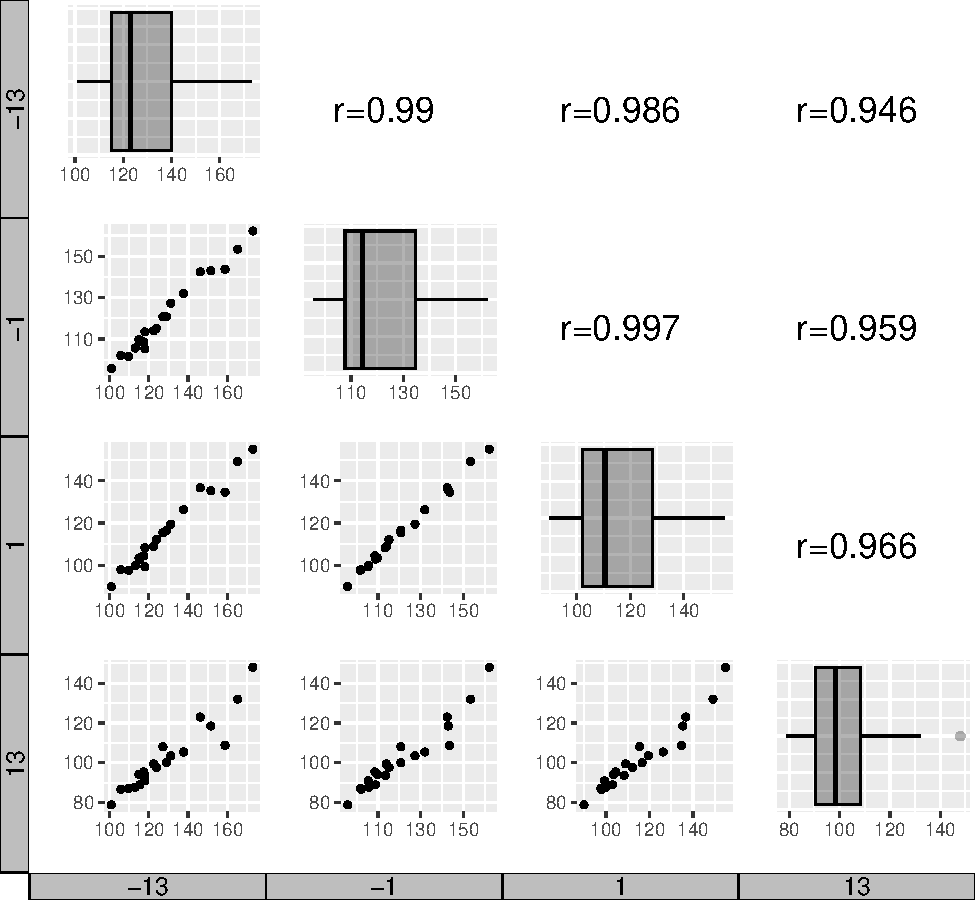
\includegraphics[trim={0 0 0 0},width=\textwidth]{./figures/scatterplot.pdf}
\end{center}
\end{minipage}
\begin{minipage}{0.48\linewidth}
\begin{center}
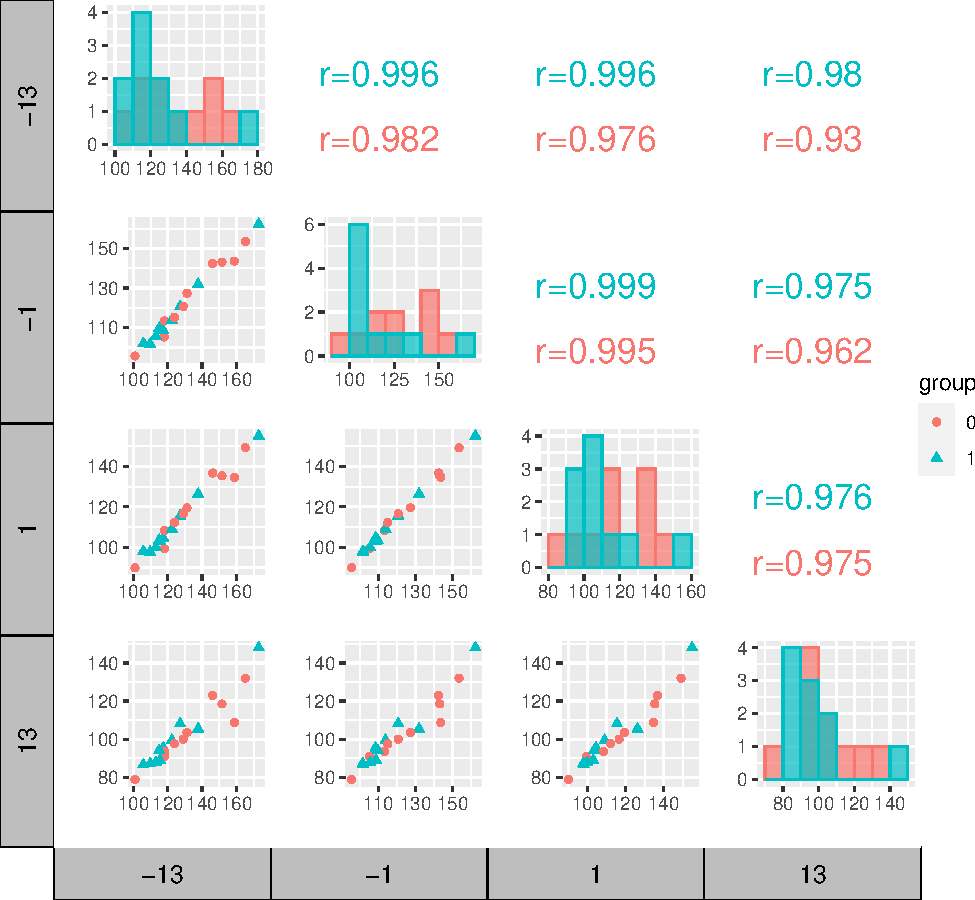
\includegraphics[trim={0 0 0 0},width=\textwidth]{./figures/scatterplot-group.pdf}
\end{center}
\end{minipage}


\bigskip

By default the resulting object will be of class \texttt{list}. A \texttt{ggplot2}
object can be obtained by setting the argument \texttt{facet} to
\texttt{"grid2"}. This requires to have installed the package ggh4x and will
produce a slightly different graphical display.

\bigskip

There is (currently) not dedicated function to obtain spaghetti
plots. Instead one can use the ggplot2 package with the long format, e.g.:
\lstset{language=r,label= ,caption= ,captionpos=b,numbers=none}
\begin{lstlisting}
gg.spa <- ggplot(gastricbypassL, aes(x=time,y=weight,group=id,color=id))
gg.spa <- gg.spa + geom_point() + geom_line()
gg.spa
\end{lstlisting}

\clearpage

\subsection{Missing data patterns}
\label{sec:orged86c41}

The \texttt{summarizeNA} function identifies the possible combinations of
observed/missing data:
\lstset{language=r,label= ,caption= ,captionpos=b,numbers=none}
\begin{lstlisting}
mp <- summarizeNA(gastricbypassL)
mp
\end{lstlisting}

\begin{verbatim}
frequency missing.pattern n.missing id visit time weight glucagonAUC group baseline
       78         0000000         0  0     0    0      0           0     0        0
        2         0000100         1  0     0    0      0           1     0        0
\end{verbatim}


A graphical representation can be obtained using \texttt{plot}:
\lstset{language=r,label= ,caption= ,captionpos=b,numbers=none}
\begin{lstlisting}
plot(mp)
\end{lstlisting}

See \texttt{help(plot.summarizeNA)} for options to customize the graphical
display.

\begin{center}
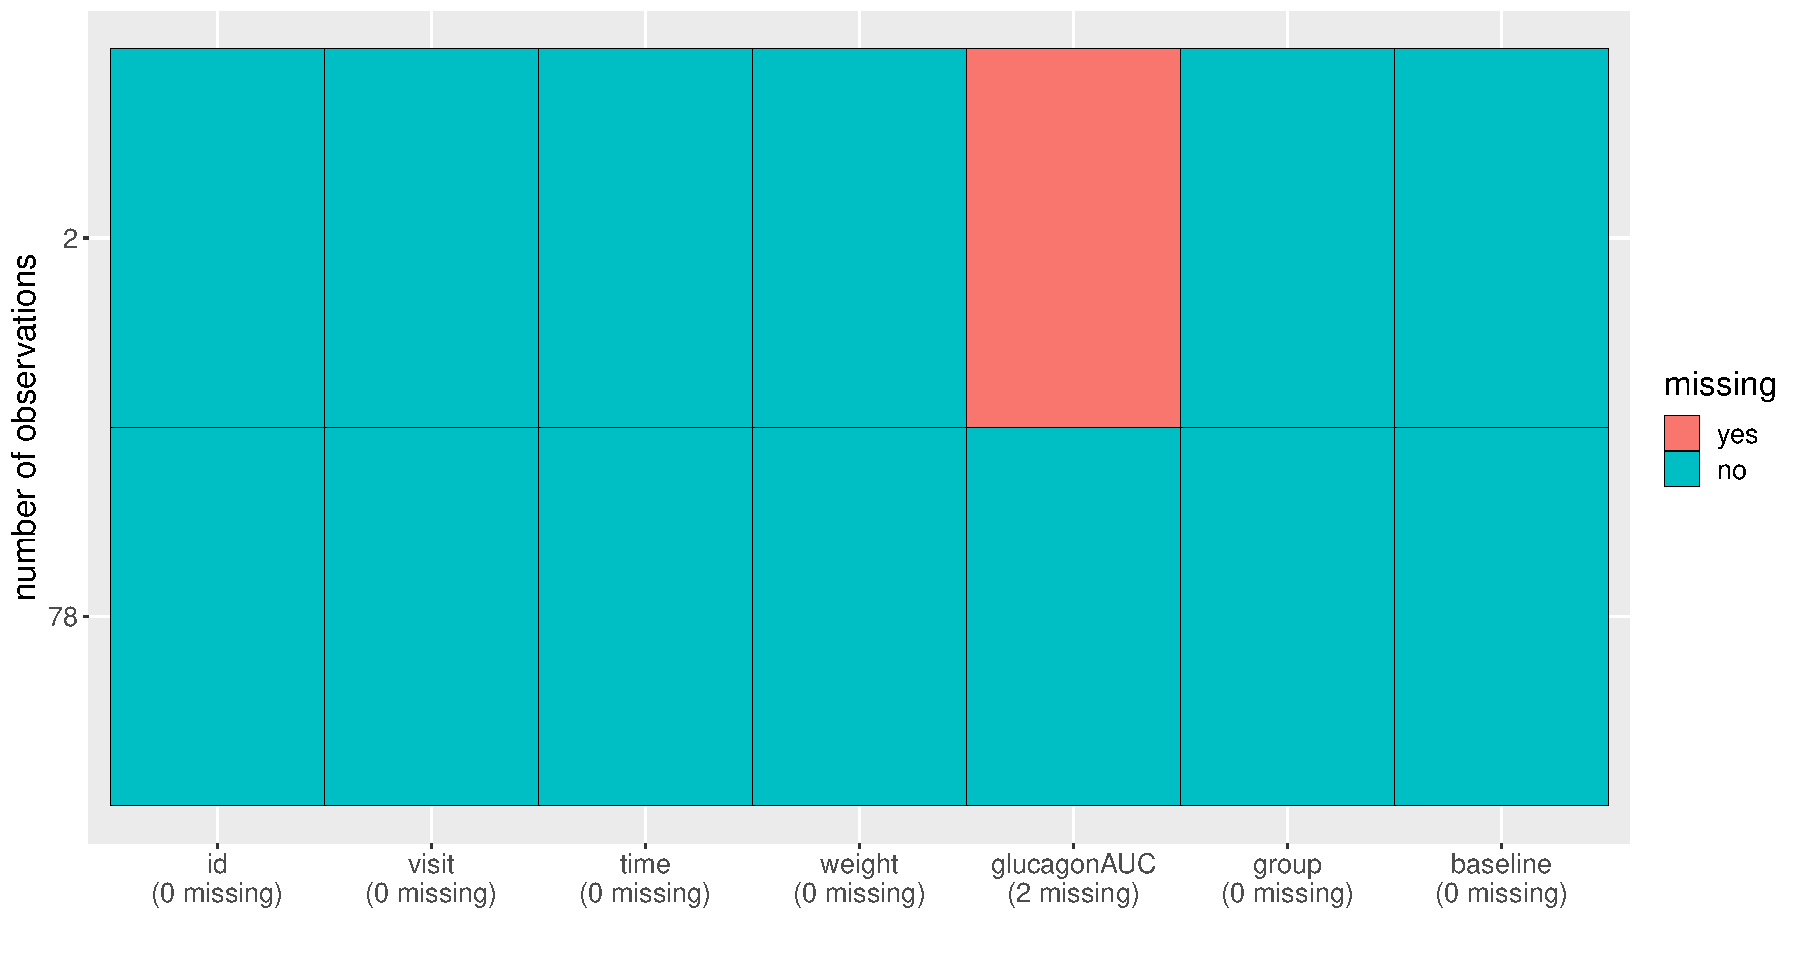
\includegraphics[trim={0 0 0 0},width=1\textwidth]{./figures/summarizeNA.pdf}
\end{center}



\clearpage

\subsection{Summary statistics}
\label{sec:orgb1611b1}

Mean, standard deviation, and other summary statistic can be computed
with respect to a categorical variable (typically time) using the
\texttt{summarize} function: \newline (\Warning this function has the same
name as a function from the dplyr package. If you have loaded dplyr,
you should use \texttt{LMMstar:::summarize})
\lstset{language=r,label= ,caption= ,captionpos=b,numbers=none}
\begin{lstlisting}
sss <- summarize(weight+glucagonAUC ~ time, data = gastricbypassL, na.rm = TRUE)
print(sss, digits = 3)
\end{lstlisting}

\begin{verbatim}
      outcome time observed missing  mean   sd    min    q1 median    q3   max
1      weight  -13       20       0 129.0 20.3 100.90 115.3  123.1 139.8 173.0
2               -1       20       0 121.2 18.9  95.70 107.8  114.5 134.5 162.2
3                1       20       0 115.7 18.3  89.90 102.2  110.6 128.4 155.0
4               13       20       0 102.4 17.1  78.80  90.4   98.5 108.2 148.0
5 glucagonAUC  -13       20       0  32.3 15.5  10.28  21.3   27.9  42.5  69.1
6               -1       19       1  29.7 13.7   9.87  21.2   25.8  33.6  67.7
7                1       19       1  76.9 27.9  35.85  56.5   73.8  91.9 135.9
8               13       20       0  52.0 21.0  21.37  37.2   51.2  57.9 109.2
\end{verbatim}


\noindent Specifying a cluster (\texttt{id}) and ordering variable (\texttt{time})
enable to output correlation matrices: \newline (\Warning there should be
no duplicated value of the ordering variable within cluster)
\lstset{language=r,label= ,caption= ,captionpos=b,numbers=none}
\begin{lstlisting}
sss2 <- summarize(weight ~ time|id, data = gastricbypassL, na.rm = TRUE)
print(sss2, digits = 3)
\end{lstlisting}

\begin{verbatim}
  time observed missing mean   sd   min    q1 median  q3 max
1  -13       20       0  129 20.3 100.9 115.3  123.1 140 173
2   -1       20       0  121 18.9  95.7 107.8  114.5 135 162
3    1       20       0  116 18.3  89.9 102.2  110.6 128 155
4   13       20       0  102 17.1  78.8  90.4   98.5 108 148

 Pearson's correlation: 
      -13    -1     1    13
-13 1.000 0.990 0.986 0.946
-1  0.990 1.000 0.997 0.959
1   0.986 0.997 1.000 0.966
13  0.946 0.959 0.966 1.000
\end{verbatim}

Graphical displays of the summary statistics can be obtained via the
\texttt{plot} method, where the argument \texttt{type} specifies the summary
statistic to be displayed:
\lstset{language=r,label= ,caption= ,captionpos=b,numbers=none}
\begin{lstlisting}
plot(sss2, type = "mean") ## left panel
plot(sss2, type = "sd") ## middle panel
plot(sss2, type = "cor") ## right panel
\end{lstlisting}

See \texttt{help(plot.summarize)} for options to customize the graphical
display.

\begin{center}
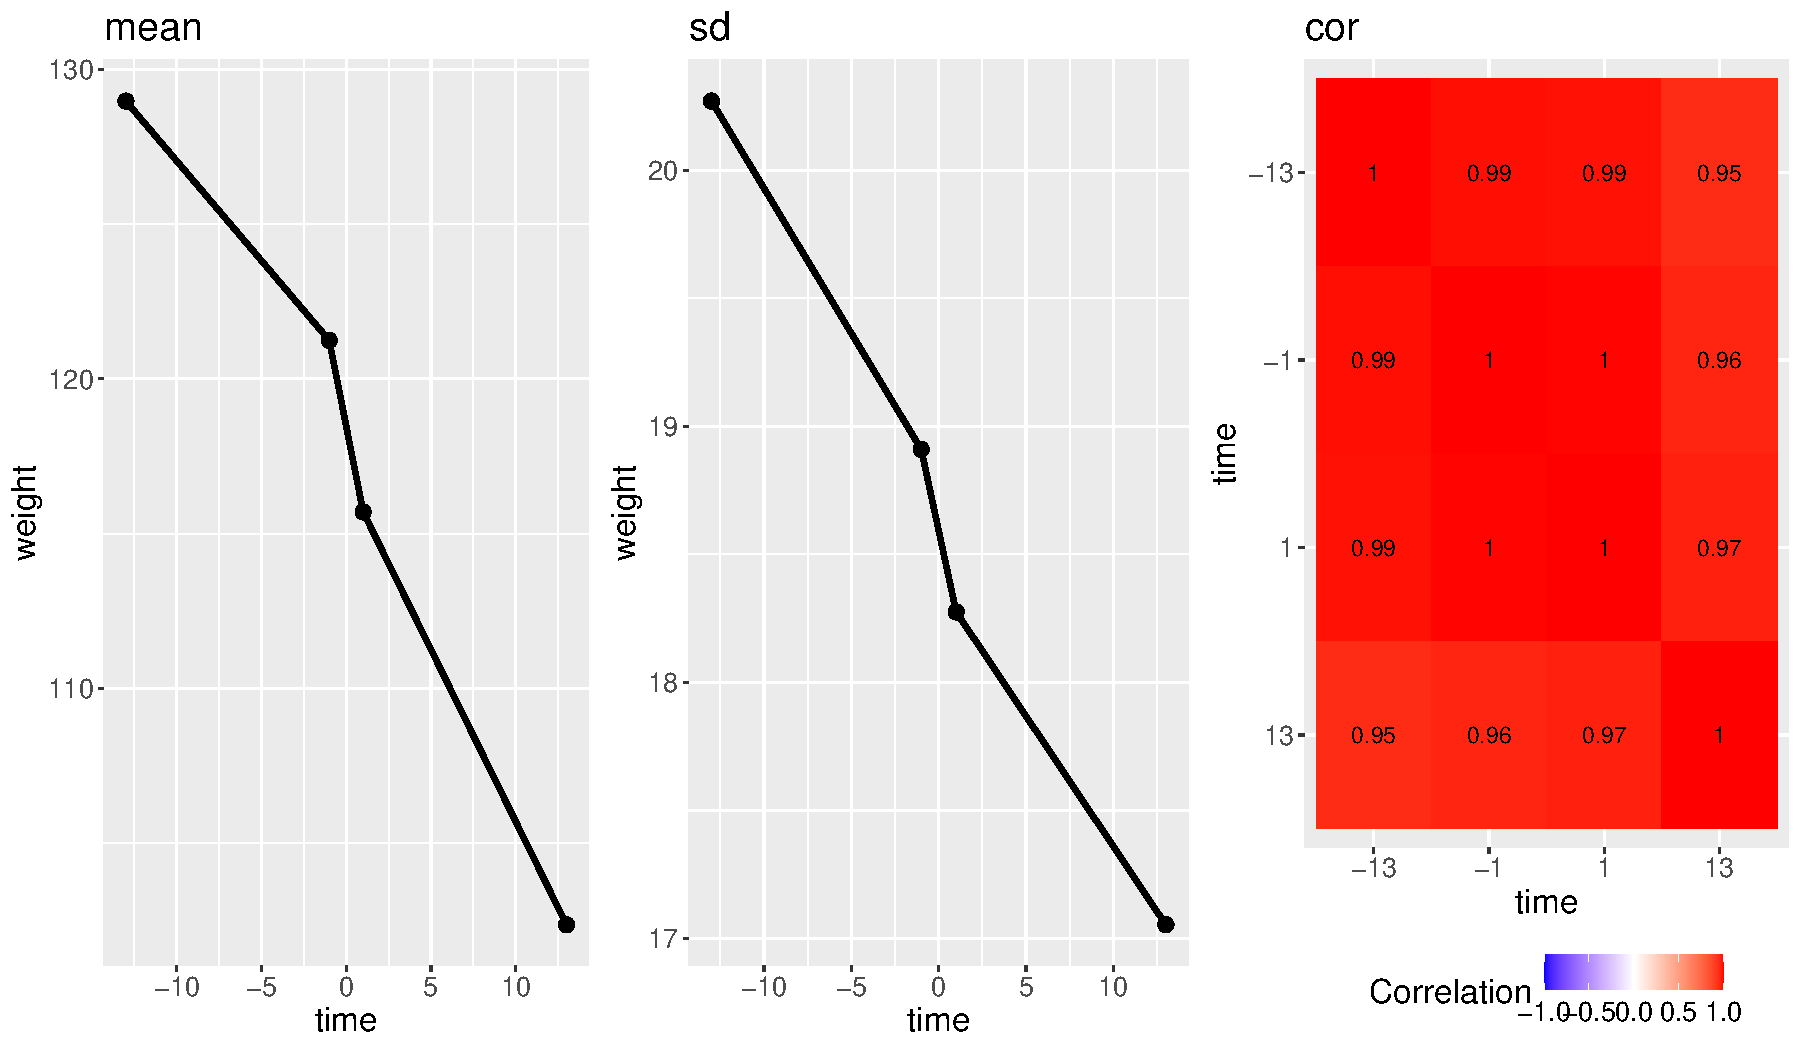
\includegraphics[trim={0 0 0 0},width=1\textwidth]{./figures/summarize.pdf}
\end{center}

\clearpage

\subsection{Correlation and partial correlations}
\label{sec:org849acc4}

The \texttt{partialCor} function can be used to evaluate group-specific
correlations, e.g.:
\lstset{language=r,label= ,caption= ,captionpos=b,numbers=none}
\begin{lstlisting}
partialCor(weight + glucagonAUC ~ 1, by = "group", data = gastricbypassL)
\end{lstlisting}

\begin{verbatim}
                           estimate    se   df  lower    upper p.value
0: rho(weight,glucagonAUC)   -0.328 0.143 21.8 -0.587 -0.00886  0.0447
1: rho(weight,glucagonAUC)   -0.354 0.141 22.5 -0.607 -0.03631  0.0313
\end{verbatim}


This willl lead to the same estimate as the \texttt{cor.test} function
(Pearson correlation):
\lstset{language=r,label= ,caption= ,captionpos=b,numbers=none}
\begin{lstlisting}
gastricbypassL.0 <- gastricbypassL[gastricbypassL$group==0,]
rho <- cor.test(gastricbypassL.0$weight, gastricbypassL.0$glucagonAUC)
c(rho$estimate, p.value = rho$p.value)
\end{lstlisting}

\begin{verbatim}
      cor   p.value 
-0.328481  0.038505
\end{verbatim}


However the p-value may differ, especially in small samples, as
\texttt{partialCor} uses a different (and probably more crude) small sample
approximation for the estimator's distribution. Nevertheless
\texttt{partialCor} enables to compare correlation coefficients across
groups, by specifying the argument \texttt{effects}:
\lstset{language=r,label= ,caption= ,captionpos=b,numbers=none}
\begin{lstlisting}
partialCor(weight + glucagonAUC ~ 1, by = "group", effects = "Dunnett",
           data = gastricbypassL)
\end{lstlisting}

\begin{verbatim}
                                                      estimate se df lower upper p.value
1:rho(weight,glucagonAUC) - 0:rho(weight,glucagonAUC)  -0.0255 NA NA    NA    NA   0.899
\end{verbatim}



Partial correlations can be also computed by specifying covariate to
adjust for on the right-hand side:
\lstset{language=r,label= ,caption= ,captionpos=b,numbers=none}
\begin{lstlisting}
partialCor(weight4 + glucagonAUC4 ~ weight1,
           data = gastricbypassW)
\end{lstlisting}

\begin{verbatim}
                          estimate    se   df  lower upper p.value
rho(weight4,glucagonAUC4)    0.112 0.233 9.12 -0.397 0.568   0.645
\end{verbatim}


When the set of covariates is outcome-dependent, a list of formulas
can be used instead:
\lstset{language=r,label= ,caption= ,captionpos=b,numbers=none}
\begin{lstlisting}
partialCor(list(weight1 ~ glucagonAUC1, weight4 ~ glucagonAUC4),
           data = gastricbypassW)
\end{lstlisting}

\begin{verbatim}
                     estimate     se   df lower upper  p.value
rho(weight1,weight4)    0.946 0.0252 26.4 0.861 0.979 5.51e-08
\end{verbatim}


These partial correlations are defined as the residual correlation
between the outcomes, i.e. the correlation once the covariate effects
have been substracted from the outcome, and a linear mixed model is
used to estimated them.

\clearpage

\section{Multiple Student's t-tests}
\label{sec:orgc4438d1}

When working with multiple outcomes and having no missing data, mean
comparisons between exposure groups can be carried out using Student's
t-tests at each timepoint, e.g.:
\lstset{language=r,label= ,caption= ,captionpos=b,numbers=none}
\begin{lstlisting}
restt <- t.test(weight1 ~ group, data = gastricbypassW)
c(estimate = unname(diff(restt$estimate)), p.value = restt$p.value)
\end{lstlisting}

\begin{verbatim}
 estimate   p.value 
-10.60000   0.25282
\end{verbatim}


And so on for the three other timepoints. Morever results would
typically need to be adjusted for multiple comparisons, e.g. when
looking for any mean difference. This can be faciliated by
\lstset{language=r,label= ,caption= ,captionpos=b,numbers=none}
\begin{lstlisting}
## single step max-test adjustment (see help(confint.Wald_lmm) for details)
mt.test(weight1+weight2+weight3+weight4~group, data = gastricbypassW)
\end{lstlisting}

\begin{verbatim}
       by parameter estimate     se     df   lower   upper p.value
1 weight1     group   -10.60 8.9717 17.965 -30.968  9.7680 0.31894
2 weight2     group    -9.50 8.3951 17.985 -28.559  9.5590 0.34164
3 weight3     group    -8.92 8.1295 17.959 -27.376  9.5358 0.35891
4 weight4     group    -4.59 7.7607 17.682 -22.209 13.0286 0.66331
\end{verbatim}


The method used to adjust confidence intervals and p-values for
multiple comparisons can be specified via the \texttt{method} argument, e.g.:
\lstset{language=r,label= ,caption= ,captionpos=b,numbers=none}
\begin{lstlisting}
## no adjustment
mt.test(weight1+weight2+weight3+weight4~group, data = gastricbypassW, method = "none")
\end{lstlisting}

\begin{verbatim}
       by parameter estimate     se     df   lower   upper p.value
1 weight1     group   -10.60 8.9717 17.965 -29.452  8.2516 0.25281
2 weight2     group    -9.50 8.3951 17.985 -27.139  8.1386 0.27266
3 weight3     group    -8.92 8.1295 17.959 -26.002  8.1622 0.28703
4 weight4     group    -4.59 7.7607 17.682 -20.916 11.7356 0.56171
\end{verbatim}


\lstset{language=r,label= ,caption= ,captionpos=b,numbers=none}
\begin{lstlisting}
## bonferroni adjustment
mt.test(weight1+weight2+weight3+weight4~group, data = gastricbypassW, method = "bonferroni")
\end{lstlisting}

\begin{verbatim}
       by parameter estimate     se     df   lower  upper p.value
1 weight1     group   -10.60 8.9717 17.965 -35.498 14.298       1
2 weight2     group    -9.50 8.3951 17.985 -32.795 13.795       1
3 weight3     group    -8.92 8.1295 17.959 -31.481 13.641       1
4 weight4     group    -4.59 7.7607 17.682 -26.165 16.985       1
\end{verbatim}



\clearpage

\section{Linear mixed model (LMM)}
\label{sec:orga3f96f5}
\subsection{Classical covariance patterns}
\label{sec:org3de11e0}

Several build-in covariance patterns can be used when specifying the
linear model. The most basic ones are the \textbf{identity} structure:
\lstset{language=r,label= ,caption= ,captionpos=b,numbers=none}
\begin{lstlisting}
eId.lmm <- lmm(glucagonAUC ~ visit*group, repetition = ~time|id, 
               structure = "ID", data = gastricbypassL)
eId.lmm
cat(" modeled residual variance-covariance: \n");sigma(eId.lmm)
\end{lstlisting}

\begin{verbatim}
		Linear regression 

 outcome/cluster/time: glucagonAUC/id/time 
 data                : 78 observations from 20 clusters 
 parameter           : 8 mean ((Intercept) visit2 visit3 visit4 group1 visit2:group1 visit3:group1 visit4:group1) 
                       1 variance (sigma) 
 log-restr.likelihood: -316.461119970244 
 convergence         : TRUE (0 iterations)
 modeled residual variance-covariance: 
       -13     -1      1     13
-13 381.35   0.00   0.00   0.00
-1    0.00 381.35   0.00   0.00
1     0.00   0.00 381.35   0.00
13    0.00   0.00   0.00 381.35
\end{verbatim}

and the \textbf{independence} structure:
\lstset{language=r,label= ,caption= ,captionpos=b,numbers=none}
\begin{lstlisting}
eInd.lmm <- lmm(glucagonAUC ~ visit*group, repetition = ~time|id, 
                structure = "IND", data = gastricbypassL)
eInd.lmm
cat(" modeled residual variance-covariance: \n");sigma(eInd.lmm)
\end{lstlisting}

\begin{verbatim}
		Linear regression with heterogeneous residual variance 

 outcome/cluster/time: glucagonAUC/id/time 
 data                : 78 observations from 20 clusters 
 parameter           : 8 mean ((Intercept) visit2 visit3 visit4 group1 visit2:group1 visit3:group1 visit4:group1) 
                       4 variance (sigma k.-1 k.1 k.13) 
 log-restr.likelihood: -310.428096419287 
 convergence         : TRUE (0 iterations)
 modeled residual variance-covariance: 
       -13     -1      1     13
-13 209.44   0.00   0.00   0.00
-1    0.00 174.81   0.00   0.00
1     0.00   0.00 768.23   0.00
13    0.00   0.00   0.00 382.95
\end{verbatim}

\clearpage

The most common linear mixed model uses a \textbf{compound symmetry} structure:
\lstset{language=r,label= ,caption= ,captionpos=b,numbers=none}
\begin{lstlisting}
eCS.lmm <- lmm(glucagonAUC ~ visit*group, repetition = ~time|id,
               structure = "CS", data = gastricbypassL)
eCS.lmm
cat(" modeled residual variance-covariance: \n");sigma(eCS.lmm)
\end{lstlisting}

\begin{verbatim}
		Linear Mixed Model with a compound symmetry covariance matrix 

 outcome/cluster/time: glucagonAUC/id/time 
 data                : 78 observations from 20 clusters 
 parameter           : 8 mean ((Intercept) visit2 visit3 visit4 group1 visit2:group1 visit3:group1 visit4:group1) 
                       1 variance (sigma) 
                       1 correlation (rho(id)) 
 log-restr.likelihood: -314.394203759159 
 convergence         : TRUE (6 iterations)
 modeled residual variance-covariance: 
        -13      -1       1      13
-13 380.580  82.741  82.741  82.741
-1   82.741 380.580  82.741  82.741
1    82.741  82.741 380.580  82.741
13   82.741  82.741  82.741 380.580
\end{verbatim}

\noindent A more flexible model can be obtained with a \textbf{toeplitz} covariance matrix:
\lstset{language=r,label= ,caption= ,captionpos=b,numbers=none}
\begin{lstlisting}
eTOE.lmm <- lmm(glucagonAUC ~ visit*group, repetition = ~time|id,
                structure = "TOEPLITZ", data = gastricbypassL)
eTOE.lmm
cat(" modeled residual correlation: \n");cov2cor(sigma(eTOE.lmm))
\end{lstlisting}

\begin{verbatim}
		Linear Mixed Model with a block Toeplitz covariance matrix 

 outcome/cluster/time: glucagonAUC/id/time 
 data                : 78 observations from 20 clusters 
 parameter           : 8 mean ((Intercept) visit2 visit3 visit4 group1 visit2:group1 visit3:group1 visit4:group1) 
                       4 variance (sigma k.-1 k.1 k.13) 
                       4 correlation (rho(12) rho(14) rho(26) rho(2)) 
 log-restr.likelihood: -297.525485582536 
 convergence         : TRUE (15 iterations)
 modeled residual correlation: 
          -13       -1        1        13
-13  1.000000 0.700020 0.093615 -0.082963
-1   0.700020 1.000000 0.016795  0.093615
1    0.093615 0.016795 1.000000  0.700020
13  -0.082963 0.093615 0.700020  1.000000
\end{verbatim}

\clearpage

\noindent And an even more flexible model can be obtained with an
\textbf{unstructured} covariance matrix:

\lstset{language=r,label= ,caption= ,captionpos=b,numbers=none}
\begin{lstlisting}
eUN.lmm <- lmm(glucagonAUC ~ visit*group, repetition = ~time|id,
               structure = "UN", data = gastricbypassL)
eUN.lmm
cat(" modeled residual variance-covariance: \n");sigma(eUN.lmm)
\end{lstlisting}

\begin{verbatim}
		Linear Mixed Model with an unstructured covariance matrix 

 outcome/cluster/time: glucagonAUC/id/time 
 data                : 78 observations from 20 clusters 
 parameter           : 8 mean ((Intercept) visit2 visit3 visit4 group1 visit2:group1 visit3:group1 visit4:group1) 
                       4 variance (sigma k.-1 k.1 k.13) 
                       6 correlation (rho(-13,-1) rho(-13,1) rho(-13,13) rho(-1,1) rho(-1,13) rho(1,13)) 
 log-restr.likelihood: -295.314056198772 
 convergence         : TRUE (8 iterations)
 modeled residual variance-covariance: 
        -13       -1        1      13
-13 209.442 150.2502 106.4000 -24.202
-1  150.250 168.1138   1.3064 -23.884
1   106.400   1.3064 748.0769 288.184
13  -24.202 -23.8844 288.1839 382.952
\end{verbatim}

\noindent Stratification of the covariance structure on a categorical
variable is also possible:
\begin{itemize}
\item e.g. to get a \textbf{stratified compound symmetry}
\end{itemize}
\lstset{language=r,label= ,caption= ,captionpos=b,numbers=none}
\begin{lstlisting}
eSCS.lmm <- lmm(glucagonAUC ~ visit*group, repetition = ~time|id,
                structure = CS(group~1), data = gastricbypassL)
eSCS.lmm
\end{lstlisting}

\begin{verbatim}
	       Linear Mixed Model with a stratified compound symmetry covariance matrix 

outcome/cluster/time: glucagonAUC/id/time 
data                : 78 observations from 20 clusters 
parameter           : 8 mean ((Intercept) visit2 visit3 visit4 group1 visit2:group1 visit3:group1 visit4:group1) 
                      2 variance (sigma:0 sigma:1) 
                      2 correlation (rho(id):0 rho(id):1) 
log-restr.likelihood: -314.123797063042 
convergence         : TRUE (7 iterations)
\end{verbatim}


\clearpage

\begin{itemize}
\item e.g. \textbf{stratified unstructured} covariance matrix:
\end{itemize}
\lstset{language=r,label= ,caption= ,captionpos=b,numbers=none}
\begin{lstlisting}
eSUN.lmm <- lmm(glucagonAUC ~ visit*group, repetition = ~time|id,
                structure = UN(group~1), data = gastricbypassL)
eSUN.lmm
\end{lstlisting}
\begin{verbatim}
	       Linear Mixed Model with a stratified unstructured covariance matrix 

outcome/cluster/time: glucagonAUC/id/time 
data                : 78 observations from 20 clusters 
parameter           : 8 mean ((Intercept) visit2 visit3 visit4 group1 visit2:group1 visit3:group1 visit4:group1) 
                      8 variance (sigma:0 sigma:1 k.-1:0 k.1:0 k.13:0 k.-1:1 k.1:1 k.13:1) 
                      12 correlation (rho(-13,-1):0 rho(-13,1):0 rho(-13,13):0 rho(-1,1):0 rho(-1,13):0 rho(1,13):0 rho(-13,-1):1 rho(-13,1):1 rho(-13,13):1 rho(-1,1):1 rho(-1,13):1 rho(1,13):1) 
log-restr.likelihood: -286.536815485471 
convergence         : TRUE (10 iterations)
\end{verbatim}


with modeled residual variance-covariance:

\bigskip

\begin{minipage}{0.47\linewidth}
\lstset{language=r,label= ,caption= ,captionpos=b,numbers=none}
\begin{lstlisting}
sigma(eSCS.lmm)
\end{lstlisting}

\begin{verbatim}
$`0`
        -13      -1       1      13
-13 334.289  50.782  50.782  50.782
-1   50.782 334.289  50.782  50.782
1    50.782  50.782 334.289  50.782
13   50.782  50.782  50.782 334.289

$`1`
       -13     -1      1     13
-13 428.46 115.09 115.09 115.09
-1  115.09 428.46 115.09 115.09
1   115.09 115.09 428.46 115.09
13  115.09 115.09 115.09 428.46
\end{verbatim}
\end{minipage}
\begin{minipage}{0.47\linewidth}
\lstset{language=r,label= ,caption= ,captionpos=b,numbers=none}
\begin{lstlisting}
sigma(eSUN.lmm)
\end{lstlisting}

\begin{verbatim}
$`0`
       -13      -1       1      13
-13 309.85 251.512 102.189 -42.250
-1  251.51 274.752 -79.811 -90.718
1   102.19 -79.811 579.110 163.767
13  -42.25 -90.718 163.767 173.439

$`1`
         -13     -1       1       13
-13 109.0309 48.667 104.908  -6.1549
-1   48.6665 59.395  93.976  43.2144
1   104.9077 93.976 967.583 450.8899
13   -6.1549 43.214 450.890 592.4655
\end{verbatim}
\end{minipage}

\clearpage

\noindent Finally the some covariance patterns like the compound
symmetry structure may depend on covariates:
\begin{itemize}
\item e.g. to obtain a \textbf{block compound symmetry} structure\footnote{similar to
nested random effects}:
\end{itemize}
\lstset{language=r,label= ,caption= ,captionpos=b,numbers=none}
\begin{lstlisting}
eBCS.lmm <- lmm(glucagonAUC ~ visit*group, repetition = ~time|id,
                structure = CS(~baseline, type = "homogeneous"), data = gastricbypassL)
eBCS.lmm
cat(" modeled residual variance-covariance: \n");sigma(eBCS.lmm)
\end{lstlisting}

\begin{verbatim}
		Linear Mixed Model with a block compound symmetry covariance matrix 

 outcome/cluster/time: glucagonAUC/id/time 
 data                : 78 observations from 20 clusters 
 parameter           : 8 mean ((Intercept) visit2 visit3 visit4 group1 visit2:group1 visit3:group1 visit4:group1) 
                       1 variance (sigma) 
                       2 correlation (rho(id/baseline) rho(id)) 
 log-restr.likelihood: -308.994835006264 
 convergence         : TRUE (6 iterations)
 modeled residual variance-covariance: 
        -13      -1       1      13
-13 380.957 226.403  15.465  15.465
-1  226.403 380.957  15.465  15.465
1    15.465  15.465 380.957 226.403
13   15.465  15.465 226.403 380.957
\end{verbatim}

\begin{itemize}
\item e.g. to obtain a \textbf{block unstructured} covariance matrix:
\end{itemize}
\lstset{language=r,label= ,caption= ,captionpos=b,numbers=none}
\begin{lstlisting}
eBUN.lmm <- lmm(glucagonAUC ~ visit*group, repetition = ~time|id,
                structure = CS(~baseline, type = "heterogeneous"), data = gastricbypassL)
eBUN.lmm
cat(" modeled residual variance-covariance: \n");sigma(eBUN.lmm)
\end{lstlisting}

\begin{verbatim}
		Linear Mixed Model with a block unstructured covariance matrix 

 outcome/cluster/time: glucagonAUC/id/time 
 data                : 78 observations from 20 clusters 
 parameter           : 8 mean ((Intercept) visit2 visit3 visit4 group1 visit2:group1 visit3:group1 visit4:group1) 
                       2 variance (sigma k.TRUE) 
                       3 correlation (rho(FALSE) rho(FALSE,TRUE) rho(TRUE)) 
 log-restr.likelihood: -300.047474124556 
 convergence         : TRUE (7 iterations)
 modeled residual variance-covariance: 
        -13      -1       1      13
-13 189.420 150.356  15.353  15.353
-1  150.356 189.420  15.353  15.353
1    15.353  15.353 570.908 300.071
13   15.353  15.353 300.071 570.908
\end{verbatim}

\clearpage

\subsection{User-specific covariance patterns}
\label{sec:org420293f}

It is possible input user-specific covariance patterns under the
following model for the residuals: \[\Omega =
\trans{\boldsymbol{\sigma}} R \boldsymbol{\sigma}\]
\begin{itemize}
\item \(\boldsymbol{\sigma}=f(\boldsymbol{\theta}_{\sigma},Z_{\sigma})\)
is a vector of residual standard errors depending on a vector of
parameters \(\boldsymbol{\theta}_{\sigma}\) and possible covariates
via the design matrix \(Z_{\sigma}\).
\item \(R=g(\boldsymbol{\theta}_{R},Z_R)\) is a matrix of residual
correlations depending on a vector of parameters
\(\boldsymbol{\theta}_{R}\) and possible covariates via the design
matrix \(Z_R\).
\end{itemize}

\bigskip

To be more concrete, consider the following correlation matrix
\lstset{language=r,label= ,caption= ,captionpos=b,numbers=none}
\begin{lstlisting}
rho.2block <- function(p,n.time,X){
  rho <- matrix(1, nrow = n.time, ncol = n.time)
  rho[1,2] <- rho[2,1] <- rho[4,5] <- rho[5,4] <- p["rho1"]
  rho[1,3] <- rho[3,1] <- rho[4,6] <- rho[6,4] <- p["rho2"]
  rho[2,3] <- rho[3,2] <- rho[5,6] <- rho[6,5] <- p["rho3"]
  rho[4:6,1:3] <- rho[1:3,4:6] <- p["rho4"]
  return(rho)
}
Rho <- rho.2block(p = c(rho1=0.25,rho2=0.5,rho3=0.4,rho4=0.1),
                  n.time = 6)
Rho
\end{lstlisting}

\begin{verbatim}
     [,1] [,2] [,3] [,4] [,5] [,6]
[1,] 1.00 0.25  0.5 0.10 0.10  0.1
[2,] 0.25 1.00  0.4 0.10 0.10  0.1
[3,] 0.50 0.40  1.0 0.10 0.10  0.1
[4,] 0.10 0.10  0.1 1.00 0.25  0.5
[5,] 0.10 0.10  0.1 0.25 1.00  0.4
[6,] 0.10 0.10  0.1 0.50 0.40  1.0
\end{verbatim}


and the corresponding dataset:
\lstset{language=r,label= ,caption= ,captionpos=b,numbers=none}
\begin{lstlisting}
set.seed(11)
Y <- mvtnorm::rmvnorm(1000, mean = rep(0,6), sigma = Rho)
dfW <- cbind(id = 1:NROW(Y), as.data.frame(Y))
dfL <- reshape2::melt(dfW, id.vars = "id", variable.name = "time")
dfL[dfL$id %in% 1:2,]
\end{lstlisting}

\begin{minipage}{0.45\linewidth}
\begin{verbatim}
     id time      value
1     1   V1 -0.9842079
1001  1   V2 -0.3681245
2001  1   V3 -1.6174652
3001  1   V4 -1.4994103
4001  1   V5  0.7493107
5001  1   V6 -1.0719657
\end{verbatim}


\end{minipage}
\begin{minipage}{0.45\linewidth}
\begin{verbatim}
     id time      value
2     2   V1  1.2402726
1002  2   V2  0.6494215
2002  2   V3  0.3272105
3002  2   V4 -1.0626973
4002  2   V5 -0.9013244
5002  2   V6 -0.6696714
\end{verbatim}


\end{minipage}

\clearpage

To estimate the corresponding mixed model we first define a new
covariance structure:
\lstset{language=r,label= ,caption= ,captionpos=b,numbers=none}
\begin{lstlisting}
myStruct <- CUSTOM(~time,
                   FCT.sigma = function(p,n.time,X){rep(p,n.time)}, ## function f
                   init.sigma = c("sigma"=1),
                   FCT.rho = rho.2block, ## function g
                   init.rho = c("rho1"=0.25,"rho2"=0.25,"rho3"=0.25,"rho4"=0.25))
\end{lstlisting}

and then call \texttt{lmm} with this structure structure:
\lstset{language=r,label= ,caption= ,captionpos=b,numbers=none}
\begin{lstlisting}
e.lmmCUSTOM <- lmm(value~time, repetition=~time|id,
                   structure = myStruct, data=dfL,
                   df = FALSE) ## df = FALSE to save computation time
logLik(e.lmmCUSTOM)
\end{lstlisting}

\begin{verbatim}
[1] -7962.243
\end{verbatim}


The optimization procedure may be slow but should eventually reaches
an optimum. We can then output the estimated correlation matrix:
\lstset{language=r,label= ,caption= ,captionpos=b,numbers=none}
\begin{lstlisting}
cov2cor(sigma(e.lmmCUSTOM))
\end{lstlisting}

\begin{verbatim}
           V1         V2         V3         V4         V5         V6
V1 1.00000000 0.24898095 0.50058994 0.09053785 0.09053785 0.09053785
V2 0.24898095 1.00000000 0.36110943 0.09053785 0.09053785 0.09053785
V3 0.50058994 0.36110943 1.00000000 0.09053785 0.09053785 0.09053785
V4 0.09053785 0.09053785 0.09053785 1.00000000 0.24898095 0.50058994
V5 0.09053785 0.09053785 0.09053785 0.24898095 1.00000000 0.36110943
V6 0.09053785 0.09053785 0.09053785 0.50058994 0.36110943 1.00000000
\end{verbatim}


\textbf{Comparison to build-in structure}: consider the following model using
a build-in compound symmetry structure:
\lstset{language=r,label= ,caption= ,captionpos=b,numbers=none}
\begin{lstlisting}
system.time(
  e.lmmDEFAULT.CS <- lmm(value~time, repetition = ~time|id,
                         structure = "CS", data = dfL,
                         df = FALSE)
)
\end{lstlisting}

\begin{verbatim}
 user  system elapsed 
0.097   0.000   0.097
\end{verbatim}


Using instead \texttt{CUSTOM} to specifying this structure:
\lstset{language=r,label= ,caption= ,captionpos=b,numbers=none}
\begin{lstlisting}
myCS <- CUSTOM(~1,
               FCT.sigma = function(p,n.time,X){rep(p,n.time)},
               init.sigma = c("sigma"=1), 
               FCT.rho = function(p,n.time,X){p+diag(1-p,n.time,n.time)},
               init.rho = c("rho"=0.5))
\end{lstlisting}

is considerably slower than using the pre-specified structure:
\lstset{language=r,label= ,caption= ,captionpos=b,numbers=none}
\begin{lstlisting}
system.time(
  e.lmmCUSTOM.CS <- lmm(value~time, repetition = ~time|id,
                        structure = myCS, data = dfL,
                        df = FALSE)
)
\end{lstlisting}

\begin{verbatim}
 user  system elapsed 
0.952   0.019   0.972
\end{verbatim}



but will lead to the same estimates:
\lstset{language=r,label= ,caption= ,captionpos=b,numbers=none}
\begin{lstlisting}
logLik(e.lmmDEFAULT.CS)
logLik(e.lmmCUSTOM.CS)
\end{lstlisting}

\begin{verbatim}
[1] -8186.859
[1] -8186.859
\end{verbatim}


There are two reasons for the slower execution time: slower evaluation
of the derivatives (since they are obtained by numerical
differentiation) and worse starting point, as reflected by the larger
number of interations needed to reach convergence:
\lstset{language=r,label= ,caption= ,captionpos=b,numbers=none}
\begin{lstlisting}
e.lmmDEFAULT.CS$opt$n.iter
e.lmmCUSTOM.CS$opt$n.iter
\end{lstlisting}

\begin{verbatim}
[1] 1
[1] 4
\end{verbatim}


Faster execution time can be obtained by specifying the first and
second derivative regarding each parameter:
\lstset{language=r,label= ,caption= ,captionpos=b,numbers=none}
\begin{lstlisting}
myCS.wD <- CUSTOM(~1,
                  FCT.sigma = function(p,n.time,X){rep(p,n.time)},
                  dFCT.sigma = function(p,n.time,X){list(sigma = rep(1,n.time))},
                  d2FCT.sigma = function(p,n.time,X){list(sigma = rep(0,n.time))},
                  init.sigma = c("sigma"=1),
                  FCT.rho = function(p,n.time,X){p+diag(1-p,n.time,n.time)},
                  dFCT.rho = function(p,n.time,X){list(rho = 1-diag(1,n.time,n.time))},
                  d2FCT.rho = function(p,n.time,X){list(rho = matrix(0,n.time,n.time))},
                  init.rho = c("rho"=0.5))
\end{lstlisting}

\lstset{language=r,label= ,caption= ,captionpos=b,numbers=none}
\begin{lstlisting}
system.time(
  e.lmmCUSTOMwD.CS <- lmm(value~time,
                          repetition = ~time|id,
                          structure = myCS.wD, 
                          data = dfL, df = FALSE
                          )
)
\end{lstlisting}

\begin{verbatim}
 user  system elapsed 
0.699   0.004   0.703
\end{verbatim}



\clearpage

\subsection{Estimation procedure}
\label{sec:org0a6a87f}

\textbf{Initialiation}: by default the mean parameters are initialized using
 Ordinary Least Squares (OLS) and the variance and correlation
 parameters are initialized by minimizing the difference between the
 observed and residuals variance-covariance matrix. These values can
 be visualized by specifying the argument \texttt{control}:
\lstset{language=r,label= ,caption= ,captionpos=b,numbers=none}
\begin{lstlisting}
eCS.lmm.bis <- update(eCS.lmm, control = list(trace = 2))
\end{lstlisting}

\begin{verbatim}
Initialization:
  (Intercept)        visit2        visit3        visit4        group1 visit2:group1 visit3:group1 
     38.72897      -4.73433      31.43303       4.52138     -12.82462       3.75946      27.00150 
visit4:group1         sigma       rho(id) 
     30.22391      19.52828       0.22819 

Loop:
******
  (Intercept)        visit2        visit3        visit4        group1 visit2:group1 visit3:group1 
     38.72897      -4.73433      31.43303       4.52138     -12.82462       3.80337      27.48103 
visit4:group1         sigma       rho(id) 
     30.22391      19.50846       0.21741 
Convergence after 6 iterations: max score=1.2413e-05 | max change in coefficient=4.5167e-06
\end{verbatim}

It is possible to input user-defined value:
\begin{itemize}
\item for all parameters (vector)
\end{itemize}
\lstset{language=r,label= ,caption= ,captionpos=b,numbers=none}
\begin{lstlisting}
init.all <- coef(eCS.lmm, effects = "all")
eCS.lmm.bis <- update(eCS.lmm, control = list(init = init.all, trace = 1))
\end{lstlisting}

\begin{verbatim}
Convergence after 0 iteration: max score=1.2413e-05
\end{verbatim}


\begin{itemize}
\item the mean parameters only (vector)
\end{itemize}
\lstset{language=r,label= ,caption= ,captionpos=b,numbers=none}
\begin{lstlisting}
init.mean <- coef(eCS.lmm, effects = "mean")
eCS.lmm.bis <- update(eCS.lmm, control = list(init = init.mean, trace = 2))
\end{lstlisting}

\begin{verbatim}
Initialization:
  (Intercept)        visit2        visit3        visit4        group1 visit2:group1 visit3:group1 
     38.72897      -4.73433      31.43303       4.52138     -12.82462       3.80337      27.48103 
visit4:group1         sigma       rho(id) 
     30.22391      19.52904       0.22849 

Loop:
******
  (Intercept)        visit2        visit3        visit4        group1 visit2:group1 visit3:group1 
     38.72897      -4.73433      31.43303       4.52138     -12.82462       3.80337      27.48103 
visit4:group1         sigma       rho(id) 
     30.22391      19.50846       0.21741 
Convergence after 6 iterations: max score=1.4893e-05 | max change in coefficient=5.3866e-06
\end{verbatim}

\begin{itemize}
\item a full data variance-covariance matrix (matrix).
\end{itemize}
\lstset{language=r,label= ,caption= ,captionpos=b,numbers=none}
\begin{lstlisting}
init.vcov <- sigma(eCS.lmm)
eCS.lmm.bis <- update(eCS.lmm, control = list(init = init.vcov, trace = 1))
\end{lstlisting}

\begin{verbatim}
Convergence after 0 iteration: max score=1.2413e-05
\end{verbatim}


\textbf{Optimizer}: by default the optimizer is a Newton Raphson algorithm
with backtracking. At each iteration:
\begin{itemize}
\item it computes the first two moments (score, information) according to
the current parameters values.
\item it updates the variance-covariance parameters according to the
gradient multiplied by the inverse of the information.
\item it updates the mean parameters by generalized least squares (using
the updated variance-covariance parameters).
\item it checks whether the log-likelihoood at the updated estimates is
well defined and higher than at the previous estimates. If this is
not the case, the step is re-run with half the update of the
variance-covariance parameters (backtracking).
\end{itemize}

One can modify the maximum number of iterations (\texttt{n.iter}), maximum
number of backtracking steps (\texttt{n.backtracking}), the maximum score
(absolute) value over all parameters (\texttt{tol.score}) and (absolute)
maximum difference in parameter value between to iterations
(\texttt{tol.param}) used to declare convergence. It is also possible to use
another optimizer (\texttt{optimizer}). All these elements should be passed
to the argument \texttt{control} of \texttt{lmm} using a list.

\clearpage

\subsection{Model output}
\label{sec:org9bae533}

The \texttt{summary} method can be used to display the main information
relative to the model fit:
\lstset{language=r,label= ,caption= ,captionpos=b,numbers=none}
\begin{lstlisting}
summary(eUN.lmm)
\end{lstlisting}

\begin{verbatim}
		Linear Mixed Model 
 
Dataset: gastricbypassL 

  - 20 clusters 
  - 78 observations were analyzed, 2 were excluded because of missing values 
  - between 3 and 4 observations per cluster 

Summary of the outcome and covariates: 

    $ glucagonAUC: num  20.7 49.9 42.4 27.5 29.2 ...
    $ visit      : Factor w/ 4 levels "1","2","3","4": 1 1 1 1 1 1 1 1 1 1 ...
    $ group      : Factor w/ 2 levels "0","1": 2 1 2 1 2 1 2 1 2 1 ...
    reference level: visit=1;group=0 

Estimation procedure 

  - Restricted Maximum Likelihood (REML) 
  - log-likelihood :-295.31
  - parameters: mean = 8, variance = 4, correlation = 6
  - convergence: TRUE (8 iterations) 
    largest |score| = 4.6771e-05 for rho(-1,1)
            |change|= 1.68033723859651e-05 for visit3:group1
 
Residual variance-covariance: unstructured 

  - correlation structure: ~0 + time 
            -13       -1       1      13
    -13  1.0000  0.80072 0.26880 -0.0855
    -1   0.8007  1.00000 0.00368 -0.0941
    1    0.2688  0.00368 1.00000  0.5384
    13  -0.0855 -0.09413 0.53842  1.0000

  - variance structure: ~time 
              standard.deviation ratio
    sigma.-13               14.5 1.000
    sigma.-1                13.0 0.896
    sigma.1                 27.4 1.890
    sigma.13                19.6 1.352
\end{verbatim}

\clearpage

\begin{verbatim}
Fixed effects: glucagonAUC ~ visit * group 
 
                  estimate     se   df   lower  upper p.value    
    (Intercept)     38.729  4.576   18  29.114 48.344 < 1e-04 ***
    visit2          -4.734  2.776 17.5 -10.577  1.109 0.10574    
    visit3          31.433   8.63 17.6  13.272 49.594 0.00192  **
    visit4           4.521  8.005   18 -12.297  21.34 0.57917    
    group1         -12.825  6.472   18 -26.422  0.773 0.06302   .
    visit2:group1    3.987  3.996 17.9   -4.41 12.383 0.33169    
    visit3:group1   27.571  12.42 17.8   1.461 53.682 0.03963   *
    visit4:group1   30.224 11.321   18   6.439 54.008 0.01562   *
    -------------------------------------------------------- 
   Signif. codes:  0 '***' 0.001 '**' 0.01 '*' 0.05 '.' 0.1 ' ' 1.
   Columns lower and upper contain 95% pointwise confidence intervals for each coefficient.
   Model-based standard errors are derived from the observed information (column se). 
   Degrees of freedom were computed using a Satterthwaite approximation (column df).
\end{verbatim}

\uline{Note:} the calculation of the degrees of freedom, especially when
using the observed information can be quite slow. Setting the
arguments \texttt{df} to \texttt{FALSE} and \texttt{type.information} to \texttt{"expected"} when
calling \texttt{lmm} should lead to a more reasonnable computation time.

\subsection{Extract estimated coefficients}
\label{sec:org5c75e6e}
The value of the estimated coefficients can be output using \texttt{coef}:
\lstset{language=r,label= ,caption= ,captionpos=b,numbers=none}
\begin{lstlisting}
coef(eUN.lmm)
\end{lstlisting}

\begin{verbatim}
  (Intercept)        visit2        visit3        visit4        group1 visit2:group1 visit3:group1 
      38.7290       -4.7343       31.4330        4.5214      -12.8246        3.9866       27.5714 
visit4:group1 
      30.2239
\end{verbatim}


Variance coefficients can be output by specifying the \texttt{effects} argument:
\lstset{language=r,label= ,caption= ,captionpos=b,numbers=none}
\begin{lstlisting}
coef(eUN.lmm, effects = "variance")
\end{lstlisting}

\begin{verbatim}
   sigma     k.-1      k.1     k.13 
14.47212  0.89592  1.88991  1.35220
\end{verbatim}


The first coefficient is the residual standard deviation at the
reference timepoint (here -13 week) and the remaining coefficient the
residual standard deviation at later timepoints relative to the
reference timepoint. It is possible to apply specific transformation
on the variance coefficients, for instance to obtain the residual
variance at each timepoint:
\lstset{language=r,label= ,caption= ,captionpos=b,numbers=none}
\begin{lstlisting}
coef(eUN.lmm, effects = "variance", transform.k = "sd")
\end{lstlisting}

\begin{verbatim}
sigma.-13  sigma.-1   sigma.1  sigma.13 
   14.472    12.966    27.351    19.569
\end{verbatim}

\subsection{Extract estimated coefficient and associated uncertainty}
\label{sec:org6f624b9}

The uncertainty about the mean coefficients can be obtained using the
\texttt{model.tables} method \footnote{it is equivalent to \texttt{confint} method
except that by default it also outputs \texttt{se} and \texttt{p.value}}:
\lstset{language=r,label= ,caption= ,captionpos=b,numbers=none}
\begin{lstlisting}
model.tables(eUN.lmm)
\end{lstlisting}

\begin{verbatim}
              estimate      se     df    lower    upper    p.value
(Intercept)    38.7290  4.5765 18.003  29.1143 48.34369 1.0891e-07
visit2         -4.7343  2.7759 17.543 -10.5772  1.10851 1.0574e-01
visit3         31.4330  8.6297 17.585  13.2719 49.59411 1.9229e-03
visit4          4.5214  8.0050 17.995 -12.2968 21.33958 5.7917e-01
group1        -12.8246  6.4721 18.003 -26.4219  0.77265 6.3015e-02
visit2:group1   3.9866  3.9957 17.937  -4.4102 12.38329 3.3169e-01
visit3:group1  27.5714 12.4199 17.831   1.4605 53.68232 3.9634e-02
visit4:group1  30.2239 11.3208 17.995   6.4394 54.00840 1.5624e-02
\end{verbatim}


Values for the all correlation parameters can be displayed
too, by specifying \texttt{effect=c("variance","correlation")}:
\lstset{language=r,label= ,caption= ,captionpos=b,numbers=none}
\begin{lstlisting}
model.tables(eUN.lmm, effect = c("variance","correlation"))
\end{lstlisting}

\begin{verbatim}
              estimate       se      df    lower    upper    p.value
sigma       14.4721183 2.412020 15.3158 10.15148 20.63170         NA
k.-1         0.8959206 0.127032 20.2671  0.66670  1.20396 0.44721963
k.1          1.8899095 0.431098 25.9157  1.18244  3.02067 0.00974152
k.13         1.3521979 0.317550 29.8074  0.83694  2.18468 0.20874407
rho(-13,-1)  0.8007214 0.085177 13.4142  0.52949  0.92343 0.00042923
rho(-13,1)   0.2688043 0.219200  7.9286 -0.26374  0.67576 0.27735748
rho(-13,13) -0.0854578 0.233981  8.5882 -0.55306  0.42309 0.72505145
rho(-1,1)    0.0036838 0.237237  8.1487 -0.49424  0.49979 0.98798445
rho(-1,13)  -0.0941328 0.233649  8.9191 -0.55697  0.41331 0.69821381
rho(1,13)    0.5384239 0.176221 10.2233  0.05058  0.81883 0.03522642
\end{verbatim}

Because these parameters are constrained (e.g. strictly positive),
they uncertainty is by default computed after transformation
(e.g. \texttt{log}) and then backtransformed. The column argument can be used
to extract more or less information, e.g.:
\lstset{language=r,label= ,caption= ,captionpos=b,numbers=none}
\begin{lstlisting}
model.tables(eUN.lmm, columns = c("estimate","p.value"))
\end{lstlisting}

\begin{verbatim}
              estimate    p.value
(Intercept)    38.7290 1.0891e-07
visit2         -4.7343 1.0574e-01
visit3         31.4330 1.9229e-03
visit4          4.5214 5.7917e-01
group1        -12.8246 6.3015e-02
visit2:group1   3.9866 3.3169e-01
visit3:group1  27.5714 3.9634e-02
visit4:group1  30.2239 1.5624e-02
\end{verbatim}


All parameters can be displayed by specifying
\texttt{effect="all"}.  The functions \texttt{add} (resp. \texttt{remove})
can be used to add (resp. remove) one or several columns from the
default display, e.g.:
\lstset{language=r,label= ,caption= ,captionpos=b,numbers=none}
\begin{lstlisting}
model.tables(eUN.lmm, columns = add("statistic"))
\end{lstlisting}

\begin{verbatim}
              estimate      se statistic     df    lower    upper    p.value
(Intercept)    38.7290  4.5765   8.46260 18.003  29.1143 48.34369 1.0891e-07
visit2         -4.7343  2.7759  -1.70552 17.543 -10.5772  1.10851 1.0574e-01
visit3         31.4330  8.6297   3.64242 17.585  13.2719 49.59411 1.9229e-03
visit4          4.5214  8.0050   0.56482 17.995 -12.2968 21.33958 5.7917e-01
group1        -12.8246  6.4721  -1.98151 18.003 -26.4219  0.77265 6.3015e-02
visit2:group1   3.9866  3.9957   0.99772 17.937  -4.4102 12.38329 3.3169e-01
visit3:group1  27.5714 12.4199   2.21995 17.831   1.4605 53.68232 3.9634e-02
visit4:group1  30.2239 11.3208   2.66977 17.995   6.4394 54.00840 1.5624e-02
\end{verbatim}

\subsection{Extract estimated residual variance-covariance structure}
\label{sec:orgd518e1c}

The method \texttt{sigma} can be used to output the modeled residual
covariance structure and then converted to a correlation matrix using
\texttt{cov2cor}:

\medskip

\begin{minipage}{0.45\linewidth}
\lstset{language=r,label= ,caption= ,captionpos=b,numbers=none}
\begin{lstlisting}
Sigma <- sigma(eUN.lmm)
Sigma
\end{lstlisting}

\begin{verbatim}
        -13      -1       1      13
-13 209.442 150.250 106.400 -24.202
-1  150.250 168.114   1.306 -23.884
1   106.400   1.306 748.077 288.184
13  -24.202 -23.884 288.184 382.952
\end{verbatim}

\end{minipage}
\begin{minipage}{0.05\linewidth}
\hphantom{x}
\end{minipage}
\begin{minipage}{0.45\linewidth}
\lstset{language=r,label= ,caption= ,captionpos=b,numbers=none}
\begin{lstlisting}
cov2cor(Sigma)
\end{lstlisting}

\begin{verbatim}
       -13     -1     1     13
-13  1.000  0.801 0.269 -0.085
-1   0.801  1.000 0.004 -0.094
1    0.269  0.004 1.000  0.538
13  -0.085 -0.094 0.538  1.000
\end{verbatim}

\end{minipage}

The method can also be used to extract the residual covariance
relative to a "known" individual:
\lstset{language=r,label= ,caption= ,captionpos=b,numbers=none}
\begin{lstlisting}
sigma(eUN.lmm, cluster = 5)
\end{lstlisting}

\begin{verbatim}
        -13      1      13
-13 209.442 106.40 -24.202
1   106.400 748.08 288.184
13  -24.202 288.18 382.952
\end{verbatim}


or for a new individual:
\lstset{language=r,label= ,caption= ,captionpos=b,numbers=none}
\begin{lstlisting}
newdata <- data.frame(id = "X", time = c("-13","-1","1","13"))
sigma(eUN.lmm, cluster = newdata)
\end{lstlisting}

\begin{verbatim}
        -13       -1        1      13
-13 209.442 150.2502 106.4000 -24.202
-1  150.250 168.1138   1.3064 -23.884
1   106.400   1.3064 748.0769 288.184
13  -24.202 -23.8844 288.1839 382.952
\end{verbatim}


\clearpage

\subsection{Marginal effects}
\label{sec:org5d41900}

The \texttt{effects} method can be used to evaluate marginal means with
respect to a categorical variable:
\begin{itemize}
\item \(\Esp[Y_t \mid \text{group}]\)
\end{itemize}
\lstset{language=r,label= ,caption= ,captionpos=b,numbers=none}
\begin{lstlisting}
effects(eUN.lmm, variable = "group")
\end{lstlisting}

\begin{verbatim}
		Average counterfactual outcome
		 w.r.t 'group' values 

                  estimate    se   df  lower   upper
   group=0(t=-13)   38.729 4.576   18 29.114  48.344
   group=0(t=-1)    33.995   4.1 17.9 25.377  42.612
   group=0(t=1)     70.162 8.649 17.7 51.968  88.356
   group=0(t=13)     43.25 6.188   18 30.249  56.251
   group=1(t=-13)   25.904 4.576   18  16.29  35.519
   group=1(t=-1)    25.157 4.167 18.7 16.425  33.889
   group=1(t=1)     84.909 8.951 18.2 66.115 103.702
   group=1(t=13)     60.65 6.188   18 47.649  73.651
\end{verbatim}

\begin{itemize}
\item \(\Esp[Y_t-Y_0 \mid \text{group}]\)
\end{itemize}
\lstset{language=r,label= ,caption= ,captionpos=b,numbers=none}
\begin{lstlisting}
effects(eUN.lmm, type = "change", variable = "group")
\end{lstlisting}

\begin{verbatim}
		Average counterfactual change in outcome
		 w.r.t 'group' values 

                  estimate    se   df   lower  upper
   group=0(dt=-1)   -4.734 2.776 17.5 -10.577  1.109
   group=0(dt=1)    31.433  8.63 17.6  13.272 49.594
   group=0(dt=13)    4.521 8.005   18 -12.297  21.34
   group=1(dt=-1)   -0.748 2.874 18.3  -6.779  5.283
   group=1(dt=1)    59.004 8.932   18  40.242 77.767
   group=1(dt=13)   34.745 8.005   18  17.927 51.563
\end{verbatim}

\begin{itemize}
\item \(\Esp[\int_0^T Y_t dt \mid \text{group}]\)
\end{itemize}
\lstset{language=r,label= ,caption= ,captionpos=b,numbers=none}
\begin{lstlisting}
effects(eUN.lmm, type = "auc", variable = "group")
\end{lstlisting}

\begin{verbatim}
	     Average counterfactual area under the outcome curve
	      w.r.t 'group' values 

             estimate      se   df    lower    upper
group=0(auc) 1220.972 104.098 17.8 1002.072 1439.873
group=1(auc) 1289.782 105.512 18.5 1068.508 1511.056
\end{verbatim}


It can also be used to contrast these marginal means:
\begin{itemize}
\item \(\Esp[Y_t \mid \text{group}=1]-\Esp[Y_t \mid \text{group}=0]\)
\end{itemize}
\lstset{language=r,label= ,caption= ,captionpos=b,numbers=none}
\begin{lstlisting}
effects(eUN.lmm, type = "difference", variable = "group")
\end{lstlisting}

\begin{verbatim}
	     Difference in average counterfactual outcome
	      w.r.t 'group' values 

                 estimate     se   df   lower  upper p.value  
group=1-0(t=-13)  -12.825  6.472   18 -26.422  0.773  0.0630 .
group=1-0(t=-1)    -8.838  5.846 18.3 -21.106   3.43  0.1477  
group=1-0(t=1)     14.747 12.447 17.9 -11.409 40.903  0.2516  
group=1-0(t=13)    17.399  8.752   18  -0.987 35.785  0.0622 .
\end{verbatim}


\begin{itemize}
\item \(\Esp[Y_t-Y_0 \mid \text{group}=1]-\Esp[Y_t-Y_0 \mid \text{group}=0]\)
\end{itemize}
\lstset{language=r,label= ,caption= ,captionpos=b,numbers=none}
\begin{lstlisting}
effects(eUN.lmm, type = c("change","difference"), variable = "group")
\end{lstlisting}

\begin{verbatim}
	     Difference in average counterfactual change in outcome
	      w.r.t 'group' values 

                 estimate     se   df lower  upper p.value  
group=1-0(dt=-1)    3.987  3.996 17.9 -4.41 12.383  0.3317  
group=1-0(dt=1)    27.571  12.42 17.8 1.461 53.682  0.0396 *
group=1-0(dt=13)   30.224 11.321   18 6.439 54.008  0.0156 *
\end{verbatim}


\begin{itemize}
\item \(\Esp[\int_0^T Y_t dt \mid \text{group}=1]-\Esp[\int_0^T Y_t dt \mid \text{group}=0]\)
\end{itemize}
\lstset{language=r,label= ,caption= ,captionpos=b,numbers=none}
\begin{lstlisting}
effects(eUN.lmm, type = c("auc","difference"), variable = "group")
\end{lstlisting}

\begin{verbatim}
	     Difference in average counterfactual area under the outcome curve
	      w.r.t 'group' values 

               estimate     se   df   lower   upper p.value  
group=1-0(auc)   68.809 148.22 18.1 -242.44 380.059   0.648
\end{verbatim}


It is possible to control the set of covariates used to condition on
via the \texttt{conditional} argument. This can be useful when considering an
interaction with a biomarker to obtain biomarker-specific effects.

\clearpage

\subsection{Random effects}
\label{sec:org7083b23}

Mixed model having a compound symmetry structure with positive
correlation parameters may be equivalent to random intercept models,
possibly with nested random effects. Indeed in some case the residual
variance-covariance matrix can then be decomposed as:
\[ \Omega = Z \Psi \trans{Z} + \Delta \]
\begin{itemize}
\item \(Z\) is the design matrix associated to the random effect (e.g. patient id)
\item \(\Psi\) is the variance-covariance of the random effects
\item \(\Delta\) the residual variance covariance conditional to the random effects.
\end{itemize}
One can the use \texttt{lme4} syntax to fit random intercept models with
\texttt{lmm}:
\lstset{language=r,label= ,caption= ,captionpos=b,numbers=none}
\begin{lstlisting}
eRI.lmm <- lmm(glucagonAUC ~ visit*group + (1|id), data = gastricbypassL)
eRI.lmm
\end{lstlisting}

\begin{verbatim}
	       Linear Mixed Model with a random intercept 

outcome/cluster/time: glucagonAUC/id/XXtimeXX 
data                : 78 observations from 20 clusters 
parameter           : 8 mean ((Intercept) visit2 visit3 visit4 group1 visit2:group1 visit3:group1 visit4:group1) 
                      1 variance (sigma) 
                      1 correlation (rho(id)) 
log-restr.likelihood: -314.394203759159 
convergence         : TRUE (6 iterations)
\end{verbatim}


It is also possible to specify cross or nested random effects, e.g.:
\lstset{language=r,label= ,caption= ,captionpos=b,numbers=none}
\begin{lstlisting}
eNRI.lmm <- lmm(glucagonAUC ~ visit*group + (1|id/baseline), data = gastricbypassL)
eNRI.lmm
\end{lstlisting}

\begin{verbatim}
	       Linear Mixed Model with nested random intercepts 

outcome/cluster/time: glucagonAUC/id/XXtimeXX 
data                : 78 observations from 20 clusters 
parameter           : 8 mean ((Intercept) visit2 visit3 visit4 group1 visit2:group1 visit3:group1 visit4:group1) 
                      1 variance (sigma) 
                      2 correlation (rho(id/baseline) rho(id)) 
log-restr.likelihood: -308.994835006264 
convergence         : TRUE (6 iterations)
\end{verbatim}


We obtain the same log-likelihood as, respectively, \texttt{eCS.lmm} and
\texttt{eBCS.lmm}. Indeed, as previously mentioned, with positive residual
correlation the random effect structure is equivalent to a compound
symmetry structure. \newline \Warning random slopes are not currently
supported in LMMstar. \newline \Warning the proposed implementation can
be very inefficient compared to \texttt{lme4}.

\bigskip

The joint distribution between the outcome \(\VY\)
and the random effects \(\Veta\) can be expressed as:
\[
\begin{bmatrix} \VY \\ \Veta \end{bmatrix} \sim \Gaus\left(\begin{bmatrix} \boldsymbol{\mu} \\ \mathbf{0} \end{bmatrix}, \begin{bmatrix} \Omega & Z \Psi \\ \Psi \trans{Z} & \Psi \end{bmatrix}\right)
\]
Denote by \(\varepsilon_i=\VY_i-\boldsymbol{\mu}_i\) the vector of
marginal residuals relative to individual \(i\), \(\Omega_i\) its
variance-covariance matrix, and \(\psi_j=(\Psi)_{jj}\) the variance of the
\(j\)-th random effect. We can re-express the expected value of the
\(j\)-th random effect for individual \(i\) as:
\[ \eta_{ij} = \psi_{j} Z_{ij} \Omega_i^{-1}\varepsilon_i \]
This is what the \texttt{ranef} method returns:

\bigskip

\begin{minipage}{0.48\linewidth}
\lstset{language=r,label= ,caption= ,captionpos=b,numbers=none}
\begin{lstlisting}
head(ranef(eRI.lmm, format = "wide"))
\end{lstlisting}

\begin{verbatim}
  id estimate
1  1 -2.51154
2  2  1.01043
3  3  6.08384
4  4 -6.62350
5  5  0.39519
6  6 -2.73384
\end{verbatim}

\end{minipage}
\begin{minipage}{0.48\linewidth}
\lstset{language=r,label= ,caption= ,captionpos=b,numbers=none}
\begin{lstlisting}
head(ranef(eNRI.lmm, format = "wide"))
\end{lstlisting}

\begin{verbatim}
  id  estimate estimate.FALSE estimate.TRUE
1  1 -0.494271       -3.50959      -3.23209
2  2  0.186051      -10.39431      12.93198
3  3  1.088409        9.36327       5.48225
4  4 -1.219596      -11.06703      -5.56784
5  5  0.081686       -0.71254       1.82672
6  6 -0.503386       -7.81700       0.95098
\end{verbatim}

\end{minipage}


It is also possible to extract the variance decomposition by setting
the argument \texttt{effects} to \texttt{"variance"}:

\medskip

\begin{minipage}{0.47\linewidth}
\lstset{language=r,label= ,caption= ,captionpos=b,numbers=none}
\begin{lstlisting}
ranef(eRI.lmm, effects = "variance",
      format = "wide")
\end{lstlisting}

\begin{verbatim}
      type absolute relative
1    total  380.580  1.00000
2       id   82.741  0.21741
3 residual  297.839  0.78259

\end{verbatim}

\end{minipage}
\begin{minipage}{0.47\linewidth}
\lstset{language=r,label= ,caption= ,captionpos=b,numbers=none}
\begin{lstlisting}
ranef(eNRI.lmm, effects = "variance",
      format = "wide")
\end{lstlisting}

\begin{verbatim}
      type absolute relative
1    total  380.957 1.000000
2       id   15.465 0.040595
3 baseline  210.938 0.553705
4 residual  154.554 0.405700
\end{verbatim}

\end{minipage}


Confidence intervals can also be obtained setting the argument \texttt{se} to
\texttt{TRUE} and \texttt{format} equal to \texttt{"long"}:
\lstset{language=r,label= ,caption= ,captionpos=b,numbers=none}
\begin{lstlisting}
head(ranef(eRI.lmm, se = TRUE))
\end{lstlisting}

\begin{verbatim}
  id estimate     se      df    lower   upper
1  1 -2.51154 2.3019 11.1302  -7.5708  2.5477
2  2  1.01043 2.1163 15.7355  -3.4821  5.5030
3  3  6.08384 2.9771  6.2085  -1.1421 13.3098
4  4 -6.62350 3.1114  5.8319 -14.2902  1.0432
5  5  0.39519 1.9661 23.8446  -3.6640  4.4543
6  6 -2.73384 2.2940 10.0189  -7.8438  2.3761
\end{verbatim}


\clearpage

\subsection{Sum of squares}
\label{sec:orgdc353e5}

\Warning The definition of the sum of squares is not straightforward with mixed
models. Intuitively summing residuals across several outcomes will be
hard to interpret unless all outcomes have the same variance. This is
why LMMstar does not provide them. Nevertheless for specific
covariance structure, namely independence and compound symmetry (with
positive correlation) structure, sum of squares can be deduced from
the \texttt{lmm} object - see appendix \ref{SM:sumSquares} for the theoretical
derivations. Importantly, with these structures the residuals can be
reparametrised as random effects plus independent residuals,
i.e. \(\Omega = Z \Psi \trans{Z} + \delta I\) where \(I\) is the
identity matrix and \(\delta\) the variance of these independent
residuals.

\bigskip

Appendix \ref{SM:sumSquares} illustrate how to extract the sum of squares
for univariate linear regression (i.e. independence structure) and
here we illustrate the case of a compound symmetry structure.  A key
step is to extract from the \texttt{lmm} object the conditional residual variance
\(\delta\):
\lstset{language=r,label= ,caption= ,captionpos=b,numbers=none}
\begin{lstlisting}
sigma2 <- coef(eCS.lmm, effect = "variance")^2
tau <- coef(eCS.lmm, effect = "correlation")*sigma2
delta <- unname(sigma2 - tau)
\end{lstlisting}

This step will typically depend on the covariance structure. The
residual sum of squares (SSE) equals the residual degrees of freedom
times the conditional variance:
\lstset{language=r,label= ,caption= ,captionpos=b,numbers=none}
\begin{lstlisting}
df.res <- df.residual(eCS.lmm)
SSE <- df.res * delta
c(df.res = df.res, SSE = SSE)
\end{lstlisting}

\begin{verbatim}
df.res    SSE 
    70  20849
\end{verbatim}


For the regression sum of squares (SSR), we first extract the mean
parameters and their variance-covariance based on the expected
information:
\lstset{language=r,label= ,caption= ,captionpos=b,numbers=none}
\begin{lstlisting}
eBeta.lmm <- coef(eCS.lmm)
eVcov.lmm <- vcov(eCS.lmm, type.information = "expected")
\end{lstlisting}

Parameters are grouped with respect to the original variable:
\lstset{language=r,label= ,caption= ,captionpos=b,numbers=none}
\begin{lstlisting}
attr(model.matrix(eCS.lmm),"assign")
\end{lstlisting}

\begin{verbatim}
[1] 0 1 1 1 2 3 3 3
\end{verbatim}


\bigskip

So we respect this grouping when computing the normalized SSR: 
\lstset{language=r,label= ,caption= ,captionpos=b,numbers=none}
\begin{lstlisting}
SSRstar.time <- eBeta.lmm[2:4] %*% solve(eVcov.lmm[2:4,2:4]) %*% eBeta.lmm[2:4] 
SSRstar.group <- eBeta.lmm[5] %*% solve(eVcov.lmm[5,5]) %*% eBeta.lmm[5] 
\end{lstlisting}
The SSR is obtained by multiplying the normalized SSR by the
conditional variance:
\lstset{language=r,label= ,caption= ,captionpos=b,numbers=none}
\begin{lstlisting}
SSR.time <- as.double(SSRstar.time * delta)
SSR.group <- as.double(SSRstar.group * delta)
c(time = SSR.time, group = SSR.group)
\end{lstlisting}
\begin{verbatim}
   time   group 
7872.19  643.57
\end{verbatim}

\subsection{Proportion of explained variance and partial correlation}
\label{sec:org2e0d5b9}

For a univariate linear model with homoschedastic residual variance,
the proportion of explained variance, also called partial \(R^2\) or
partial \(\eta^2\), is defined as the ratio between sum of squares
(e.g. \cite{lakens2013calculating}, equation 12):
\[ R^2=\frac{SSR}{SSR + SSE} \]

\lstset{language=r,label= ,caption= ,captionpos=b,numbers=none}
\begin{lstlisting}
c(SSR.time/ (SSR.time + SSE),
  SSR.group/ (SSR.group + SSE))
\end{lstlisting}

\begin{verbatim}
[1] 0.274092 0.029944
\end{verbatim}


Computing the SSR for each individual coefficients, taking its squared
root, and multiplying by the sign of the corresponding coefficient
leads to the partial correlation. This procedure extends to covariance
structures that can be reparametrised as random effects plus
independent residuals (see previous subsection) such as the compound
symmetry with non-negative correlation.
\begin{description}
\item[{\Warning}] for other covariance structures, especially when the
variance may be repetition-dependent, the definition of explained
variance/partial correlation is not straightforward.
\end{description}
\lstset{language=r,label= ,caption= ,captionpos=b,numbers=none}
\begin{lstlisting}
eCS.R2 <- partialCor(eCS.lmm, R2 = TRUE)
summary(eCS.R2)
\end{lstlisting}

\begin{verbatim}

		Partial correlation 

                 estimate    se   df  lower upper p.value
   visit2          -0.073 0.119 52.4 -0.311 0.165 0.54028
   visit3           0.438 0.089 51.4   0.26 0.616 < 1e-04
   visit4            0.07 0.119 52.4 -0.168 0.308 0.55876
   group1          -0.173 0.114 60.7 -0.402 0.056 0.13527
   visit2:group1    0.041 0.119 52.8 -0.198  0.28 0.73256
   visit3:group1    0.284 0.106   52  0.071 0.497 0.01007
   visit4:group1    0.314 0.103   52  0.107 0.521 0.00365
   ------------------------------------------------------ 
  Columns lower and upper contain 95% pointwise confidence intervals for each coefficient.
  Degrees of freedom were computed using a Satterthwaite approximation (column df). 

		Coefficient of determination (R2)

               estimate    se   df  lower upper p.value
   visit          0.274  0.08 50.5  0.114 0.434  0.0012
   group           0.03  0.04 60.7 -0.049 0.109  0.4520
   visit:group    0.147 0.073 51.7 <0.001 0.295  0.0500
   global         0.598 0.053 40.4  0.492 0.705  <1e-04
   ---------------------------------------------------- 
  Columns lower and upper contain 95% pointwise confidence intervals for each coefficient.
  Degrees of freedom were computed using a Satterthwaite approximation (column df).
\end{verbatim}

Here the line "global" refer to the R2 for all covariates, computed
based on the SSR relative to all mean parameters but the intercept.
\begin{description}
\item[{\Warning}] \texttt{partialCor} will compute values for all types of mixed
models. But their interpretation as partial correlation and
proportion of explained variance outside the compound symmetry with
non-negative correlation is questionnable.
\end{description}

\bigskip

\uline{Note:} Other software packages like \texttt{effectsize::eta\_squared} uses
another formula to estimate the partial R2:
\[ R^2=\frac{F df_{num}}{F df_{num} + df_{denom}} \]

where \(F\) denote the F-statistic, \(df_{num}\)
(resp. \(df_{denom}\)) the degrees of freedom of the numerator
(resp. denominator) of this statistic. However since the calculation
of degrees of freedom in LMM is approximate, I would expect this
approach to be less reliable than the one of \texttt{partialCor} based on the
SSR and SSE.

\lstset{language=r,label= ,caption= ,captionpos=b,numbers=none}
\begin{lstlisting}
aCS.aov <- anova(eCS.lmm)$multivariate
setNames(with(aCS.aov, statistic*df.num/(statistic*df.num+df.denom)), aCS.aov$test)
\end{lstlisting}

\begin{verbatim}
   visit       group visit:group 
0.335374    0.033811    0.186290
\end{verbatim}



\bigskip


\clearpage

\subsection{Model diagnostic}
\label{sec:org7b35a90}

The method \texttt{residuals} returns the residuals in the wide format:
\lstset{language=r,label= ,caption= ,captionpos=b,numbers=none}
\begin{lstlisting}
eUN.diagW <- residuals(eUN.lmm, type = "normalized", format = "wide")
colnames(eUN.diagW) <- gsub("normalized.","",colnames(eUN.diagW))
head(eUN.diagW)
\end{lstlisting}

\begin{verbatim}
  id    r.-13     r.-1       r.1     r.13
1  1 -0.36029 -0.11344  0.377177 -1.45539
2  2  0.77339  2.12301 -0.232908 -0.10708
3  3  1.14219 -1.44778 -0.654876  2.01259
4  4 -0.77473  0.20612 -0.127117 -1.39519
5  5  0.22435       NA  0.011432 -0.15398
6  6  0.27439 -0.67308 -1.031131  0.42724
\end{verbatim}


or in the long format:
\lstset{language=r,label= ,caption= ,captionpos=b,numbers=none}
\begin{lstlisting}
eUN.diagL <- residuals(eUN.lmm, type = "normalized", format = "long", keep.data = TRUE)
head(eUN.diagL)
\end{lstlisting}

\begin{verbatim}
  id visit time weight glucagonAUC group baseline fitted r.normalized
1  1     1  -13  127.2      20.690     1     TRUE 25.904     -0.36029
2  2     1  -13  165.2      49.922     0     TRUE 38.729      0.77339
3  3     1  -13  109.7      42.434     1     TRUE 25.904      1.14219
4  4     1  -13  146.2      27.517     0     TRUE 38.729     -0.77473
5  5     1  -13  113.1      29.151     1     TRUE 25.904      0.22435
6  6     1  -13  158.8      42.700     0     TRUE 38.729      0.27439
\end{verbatim}


Various type of residuals can be extract but the normalized one are
recommanded when doing model checking. Diagnostic plots can then be
generated by the user, or directly from the \texttt{lmm} object via the
method \texttt{plot} (which internally calls the \texttt{residuals} method):
\begin{itemize}
\item misspecification of the mean structure
\end{itemize}
\lstset{language=r,label= ,caption= ,captionpos=b,numbers=none}
\begin{lstlisting}
plot(eUN.lmm, type = "scatterplot")
\end{lstlisting}

\begin{center}
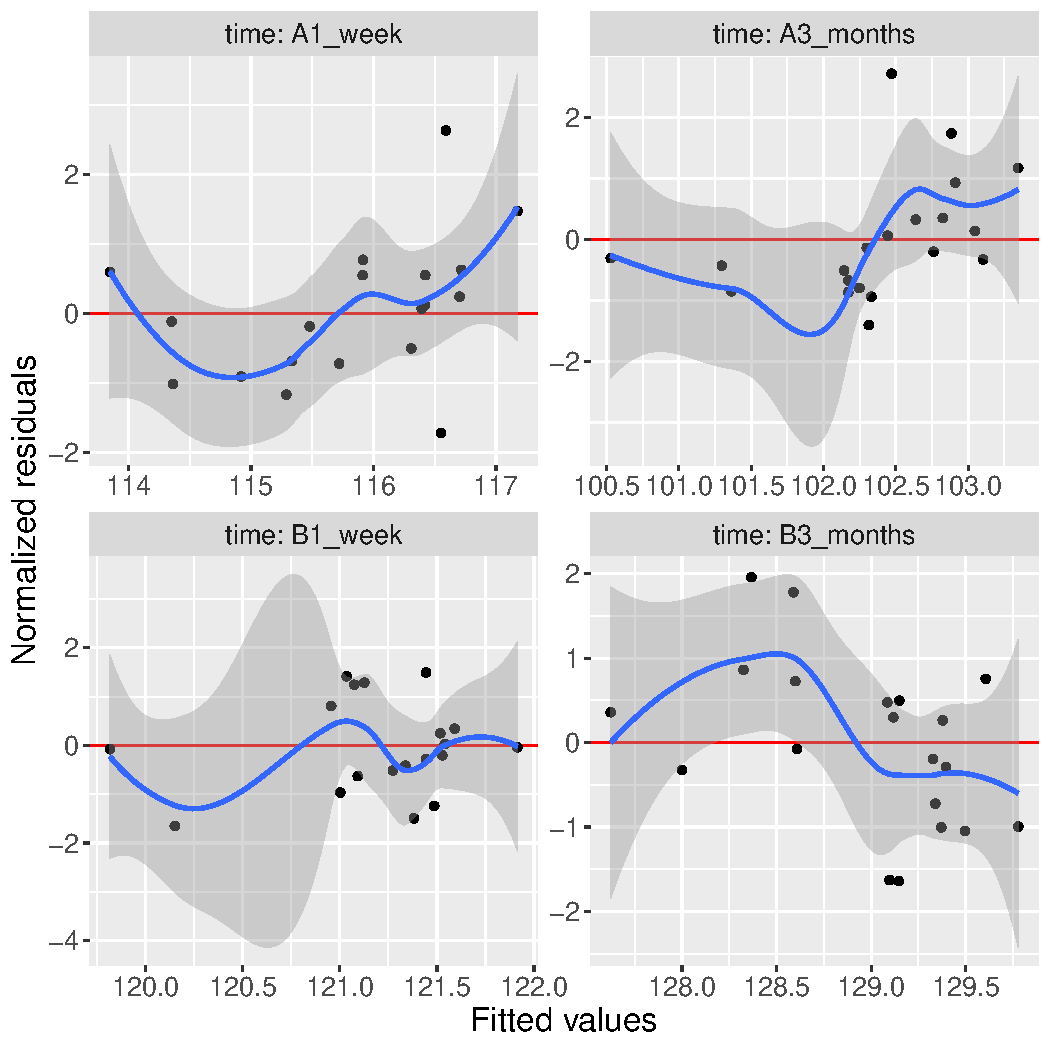
\includegraphics[width=0.4\textwidth]{./figures/diag-scatterplot.pdf}
\end{center}

\clearpage

\begin{itemize}
\item misspecification of the variance structure
\end{itemize}
\lstset{language=r,label= ,caption= ,captionpos=b,numbers=none}
\begin{lstlisting}
plot(eUN.lmm, type = "scatterplot2")
\end{lstlisting}

\begin{center}
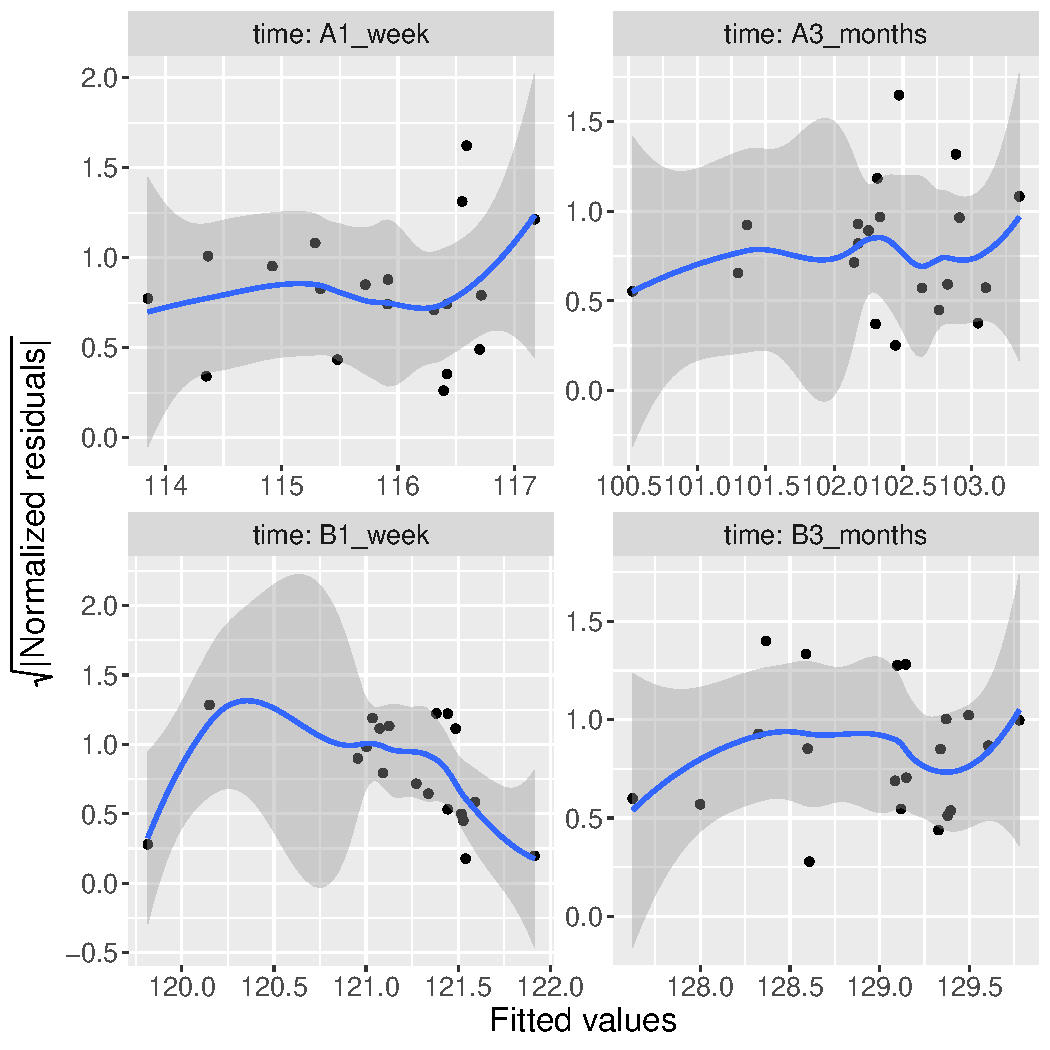
\includegraphics[width=0.4\textwidth]{./figures/diag-scatterplot2.pdf}
\end{center}

\begin{itemize}
\item misspecification of the correlation structure
\end{itemize}
\lstset{language=r,label= ,caption= ,captionpos=b,numbers=none}
\begin{lstlisting}
plot(eUN.lmm, type = "correlation", type.residual = "response")
plot(eUN.lmm, type = "correlation", type.residual = "normalized")
\end{lstlisting}

\begin{center}
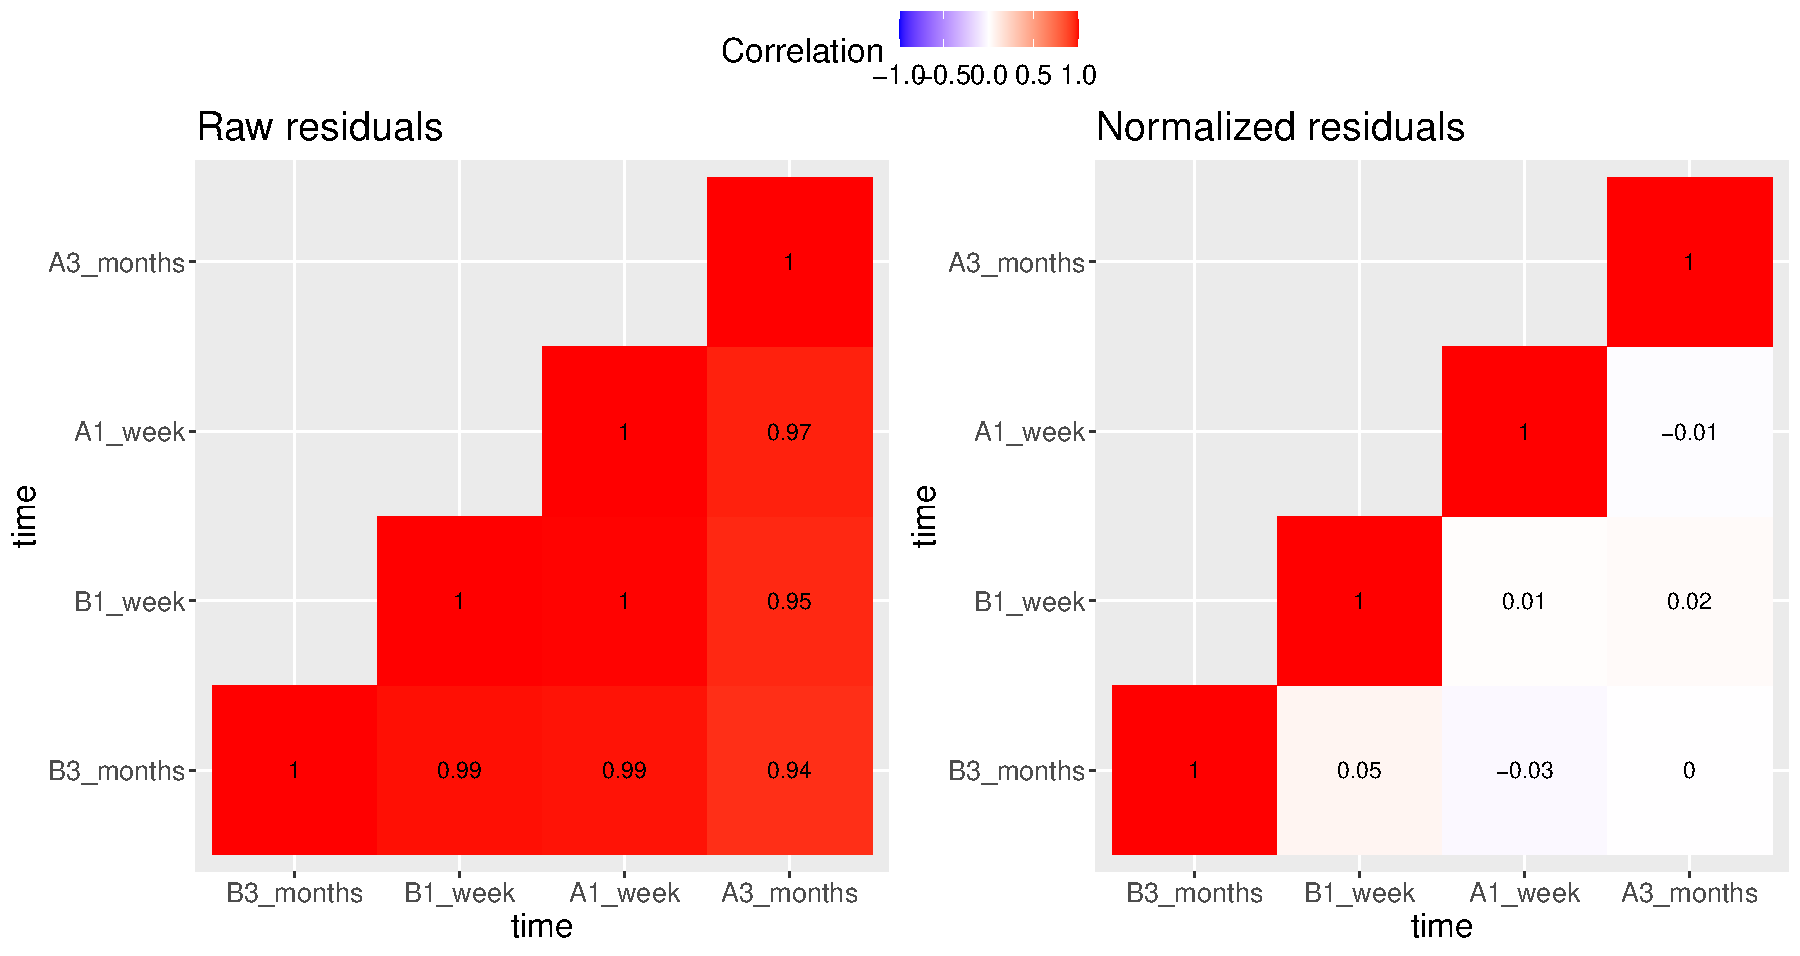
\includegraphics[width=0.6\textwidth]{./figures/diag-correlation.pdf}
\end{center}

\begin{itemize}
\item residual distribution vs. normal distribution \footnote{see \cite{oldford2016self} for guidance
about how to read quantile-quantile plots.}:
\end{itemize}

\lstset{language=r,label= ,caption= ,captionpos=b,numbers=none}
\begin{lstlisting}
plot(eUN.lmm, type = "qqplot", engine = "qqtest",
     facet = ~time, labeller = "label_both", facet_nrow=1)
## Note: the qqtest package to be installed to use the argument engine.plot = "qqtest" 
\end{lstlisting}

\begin{center}
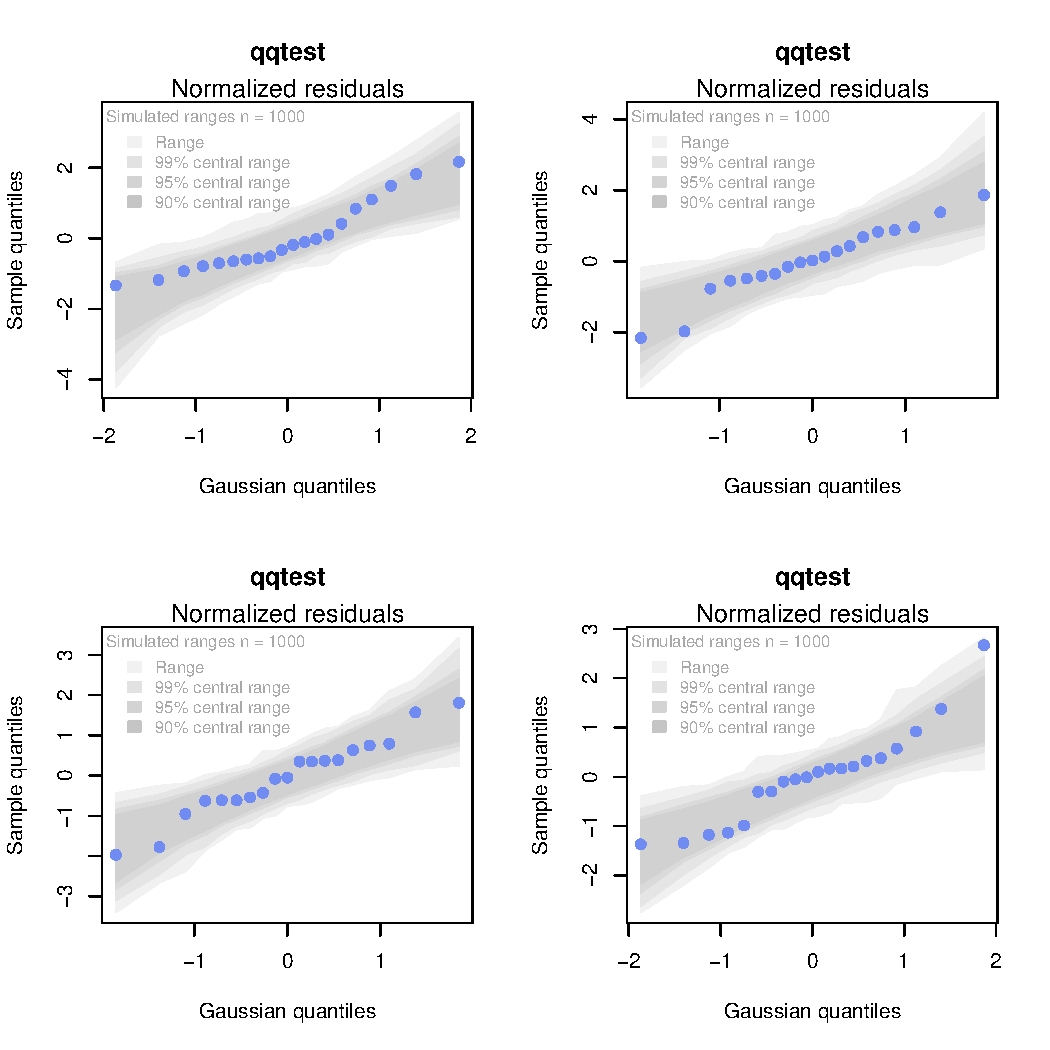
\includegraphics[width=\textwidth]{./figures/diag-qqplot.pdf}
\end{center}

\Warning Deviation from the normal distribution does not necessarily
question the validity of the statistical inference. Moreover, for
variance and correlation parameters, normally distributed data is not
enougth to ensure valid statistical inference. Instead one could
assess whether the log-likelihood is locally quadratic as this ensures
normally distributed estimates in finite samples
\citep{geyer2013asymptotics}. Since the likelihood function is a
multi-dimensional function this is not an easy task but one can look
at specific 'slices' using the \texttt{profile} method:

\lstset{language=r,label= ,caption= ,captionpos=b,numbers=none}
\begin{lstlisting}
eUN.lmm_profile <- profile(eUN.lmm, effects = c("sigma","rho(-13,-1)"))
plot(eUN.lmm_profile)
\end{lstlisting}


\begin{center}
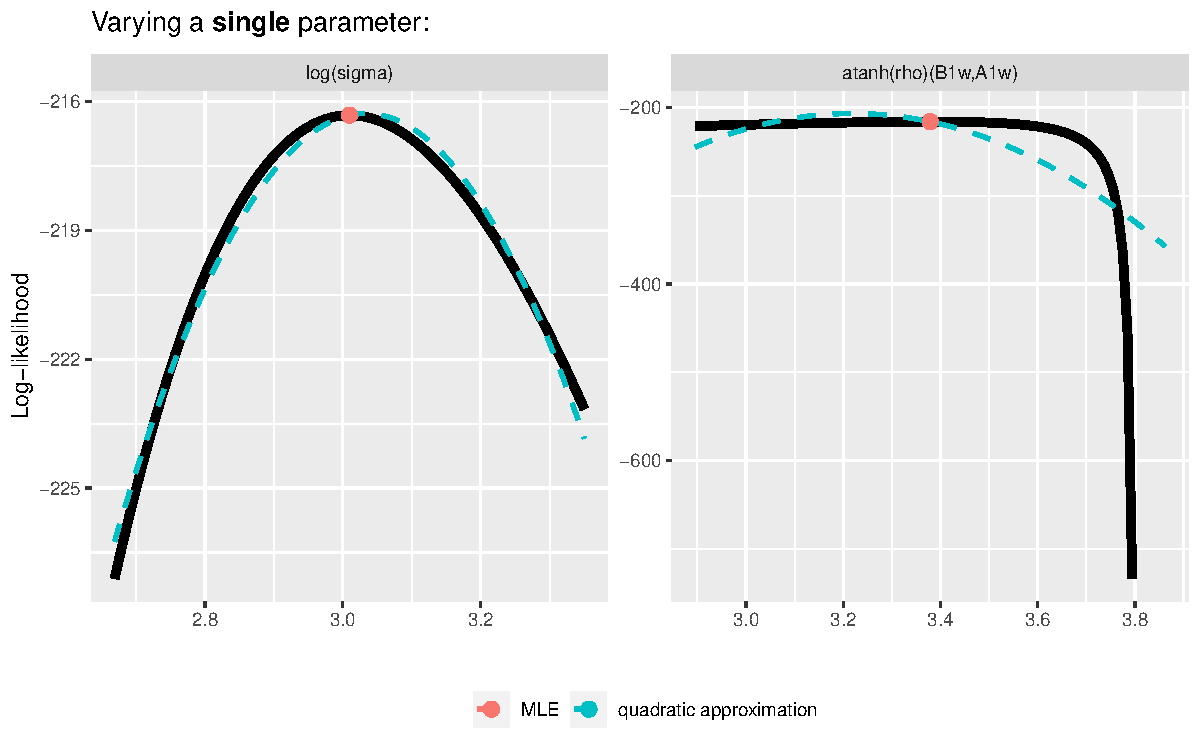
\includegraphics[width=0.75\textwidth]{./figures/diag-profileUN.pdf}
\end{center}

\clearpage

\subsection{Model fit}
\label{sec:org1968bcb}

The fitted values can be displayed via the \texttt{plot} method:
\lstset{language=r,label= ,caption= ,captionpos=b,numbers=none}
\begin{lstlisting}
## left panel
plot(eUN.lmm, type = "fit", color = "group", size.text = 20)
\end{lstlisting}

\Warning :: the shaded area represent 95\% confidence intervals (CIs),
  i.e. is not adjusted for multiplicity over time. More explicit (but
  sometimes less readable) representation of the CIs can be obtained
  by setting the argument \texttt{ci.alpha} to \texttt{NA}:

\lstset{language=r,label= ,caption= ,captionpos=b,numbers=none}
\begin{lstlisting}
## middle panel
plot(eUN.lmm, type = "fit", color = "group", ci.alpha = NA, size.text = 20)
\end{lstlisting}

\noindent It is also possible to display the observed values along with the
fitted values by setting the argument \texttt{obs.alpha} to a strictly
positive value below or equal to 1. This argument controls the
transparency of the color used to display the observed values:
\lstset{language=r,label= ,caption= ,captionpos=b,numbers=none}
\begin{lstlisting}
## right panel
plot(eUN.lmm, type = "fit", obs.alpha = 0.25, ci = FALSE, size.text = 20)
\end{lstlisting}

\begin{minipage}{0.3\linewidth}
\begin{center}
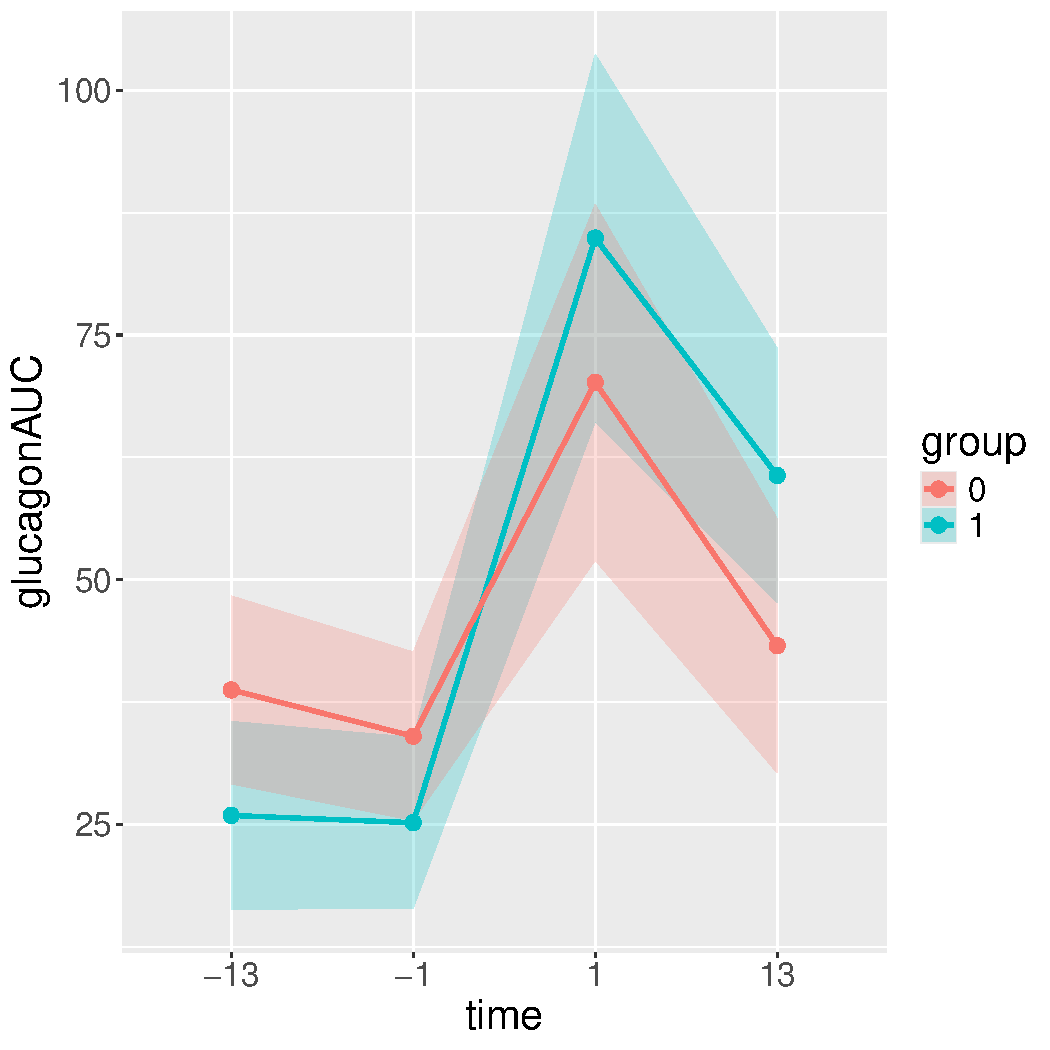
\includegraphics[width=\textwidth]{./figures/fit-autoplot.pdf}
\end{center}
\end{minipage}
\begin{minipage}{0.3\linewidth}
\begin{center}
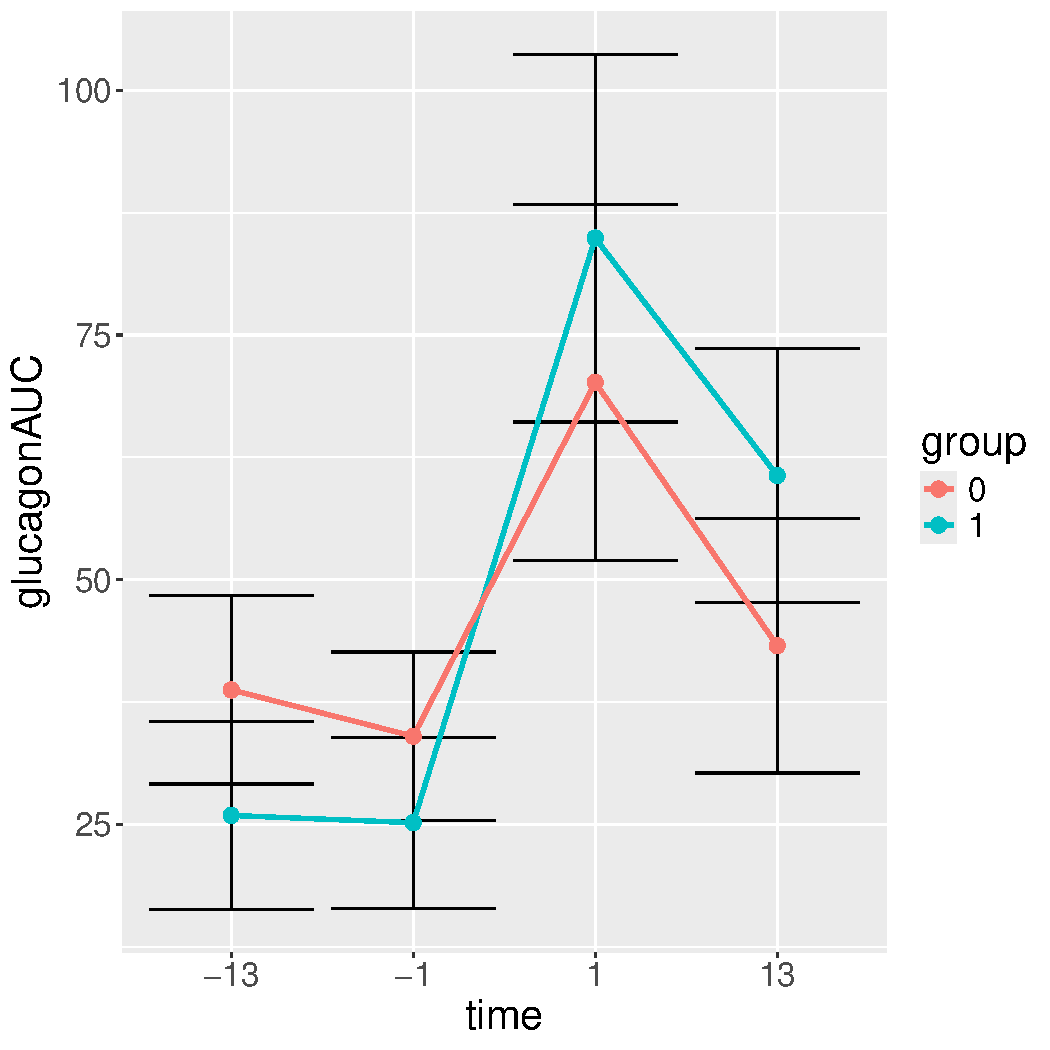
\includegraphics[width=\textwidth]{./figures/fit-autoplot2.pdf}
\end{center}
\end{minipage}
\begin{minipage}{0.3\linewidth}
\begin{center}
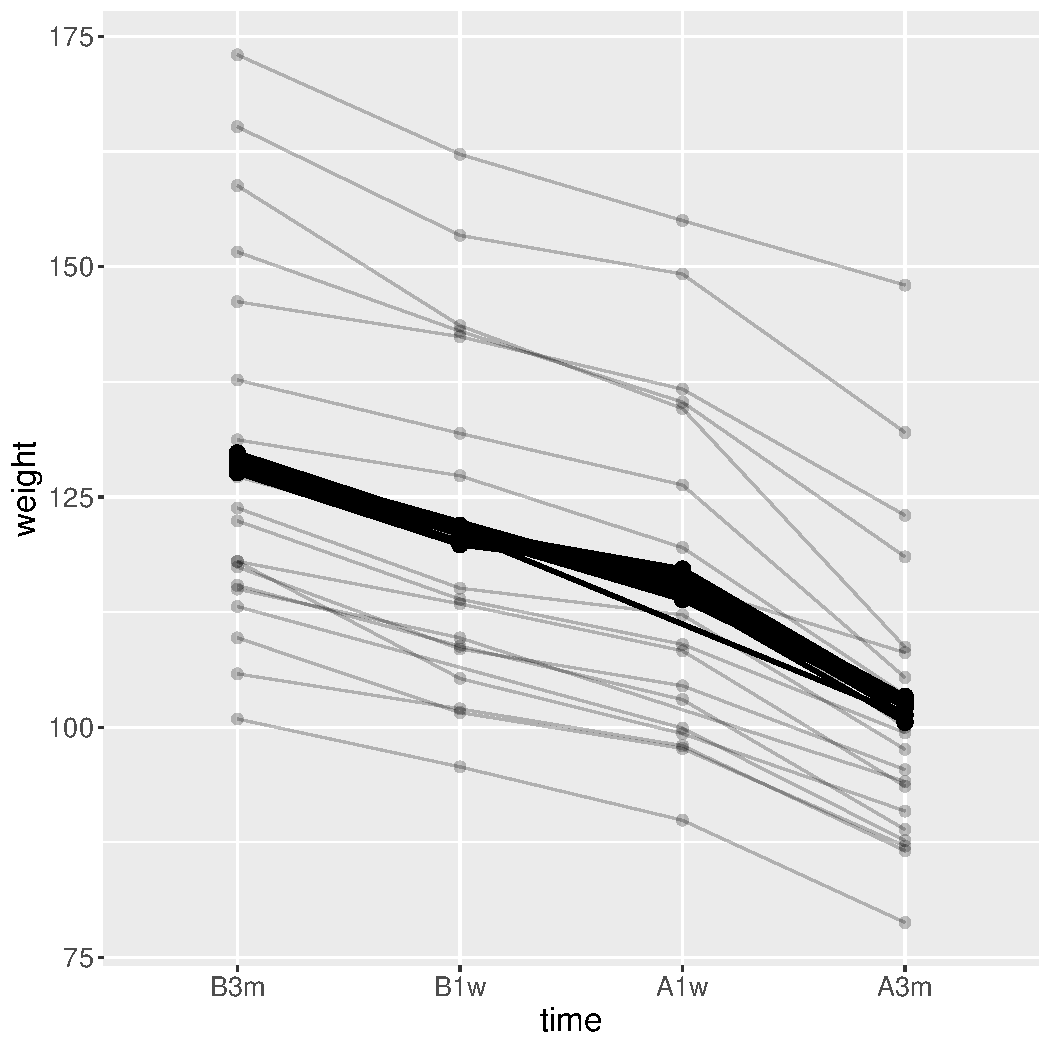
\includegraphics[width=\textwidth]{./figures/fitAll-autoplot.pdf}
\end{center}
\end{minipage}


When considering continuous covariates, e.g.:
\lstset{language=r,label= ,caption= ,captionpos=b,numbers=none}
\begin{lstlisting}
## add baseline weight
gastricbypassLB <- merge(gastricbypassL, gastricbypassW[c("id","weight1")], by = "id")

eUN.lmmB <- lmm(glucagonAUC ~ weight1 + visit*group, repetition = ~time|id,
                structure = "UN", data = gastricbypassLB)
\end{lstlisting}

The default graphical display can be confusing as it displays on curve per distinct set of covariate values: 
\lstset{language=r,label= ,caption= ,captionpos=b,numbers=none}
\begin{lstlisting}
## left panel
gg.spafit <- plot(eUN.lmmB, type = "fit", color = "group", ci = FALSE, size.text = 20)
\end{lstlisting}

However it is possible to restrict the display specific to a covariate
value via the argument \texttt{at}:
\lstset{language=r,label= ,caption= ,captionpos=b,numbers=none}
\begin{lstlisting}
## right panel
plot(eUN.lmmB, type = "fit", color = "group", ci = FALSE, size.text = 20,
     at = data.frame(weight1 = 150))
\end{lstlisting}


\begin{minipage}{0.3\linewidth}
\begin{center}
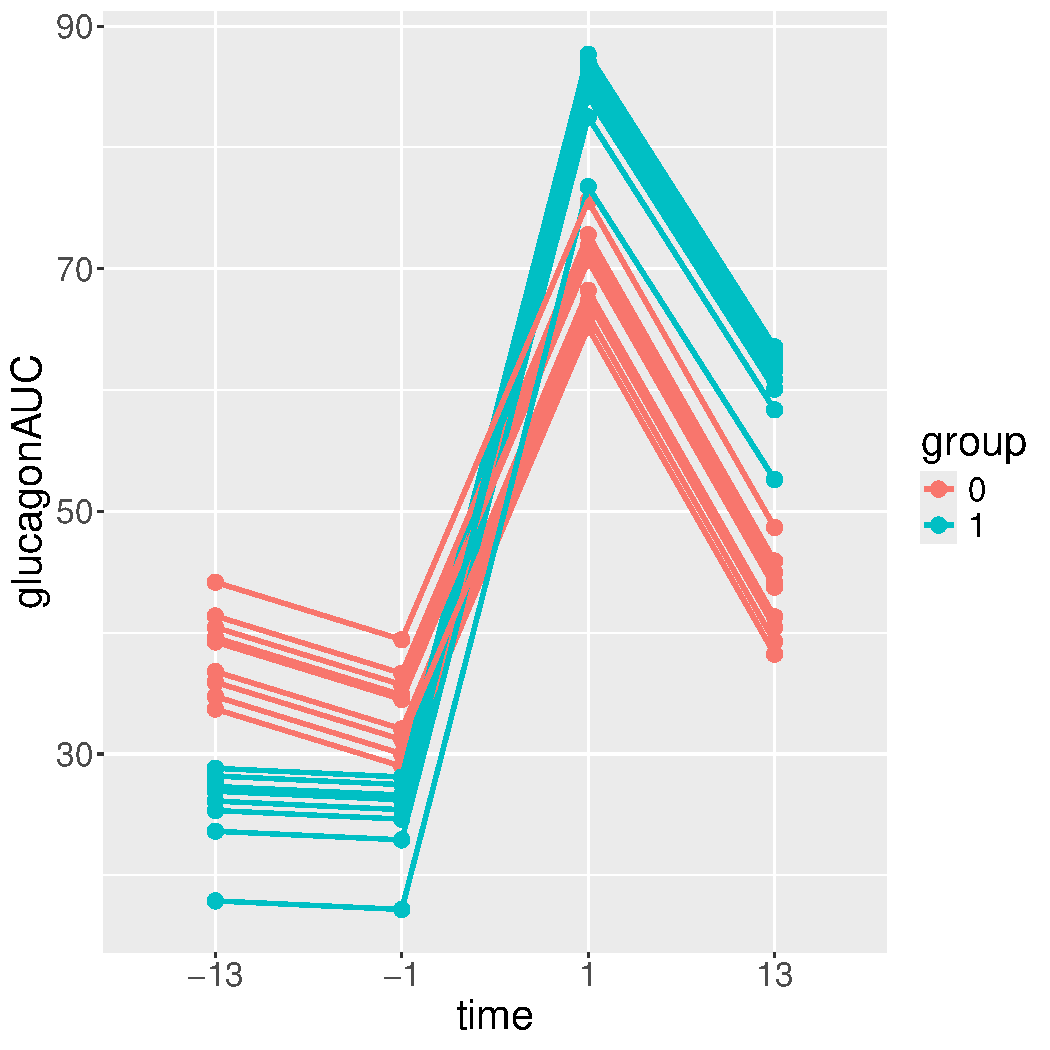
\includegraphics[width=\textwidth]{./figures/fit-baseline-autoplot.pdf}
\end{center}
\end{minipage}
\begin{minipage}{0.3\linewidth}
\begin{center}
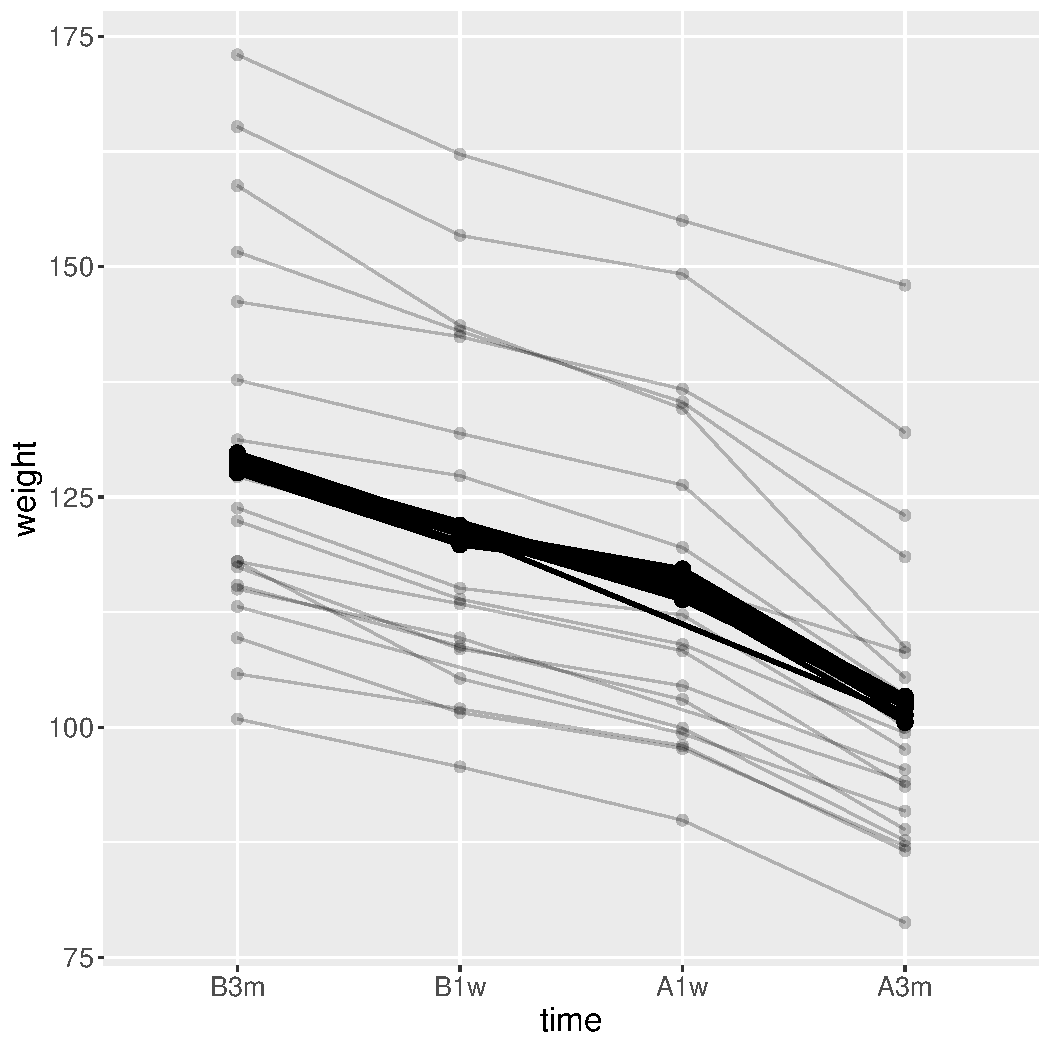
\includegraphics[width=\textwidth]{./figures/fitAll-autoplot.pdf}
\end{center}
\end{minipage}
\begin{minipage}{0.3\linewidth}
\begin{center}
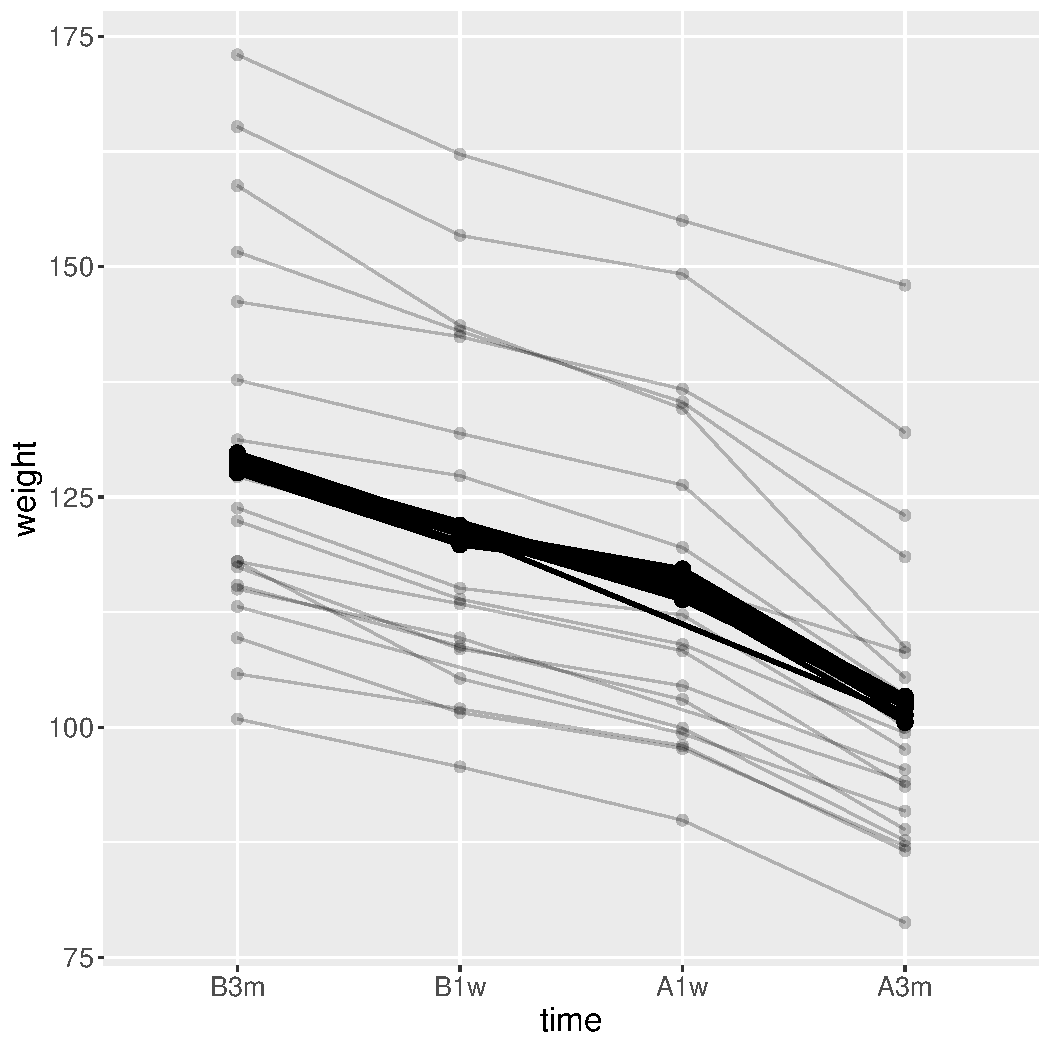
\includegraphics[width=\textwidth]{./figures/fitAll-autoplot.pdf}
\end{center}
\end{minipage}


The \texttt{plot} element output by the \texttt{plot} method can be manipulated as a ggplot object
to modify the visual appearance, e.g. to compare each individual
trajectory to the model fit:
\lstset{language=r,label= ,caption= ,captionpos=b,numbers=none}
\begin{lstlisting}
gg.traj <- gg.spafit$plot + facet_wrap(~id, labeller = label_both)
gg.traj <- gg.traj + theme(axis.text.x=element_text(angle = 90, hjust = 0))
gg.traj
\end{lstlisting}

\begin{verbatim}
Error in `combine_vars()`:
! At least one layer must contain all faceting
  variables: `id`
✖ Plot is missing `id`
✖ Layer 1 is missing `id`
✖ Layer 2 is missing `id`
Run `rlang::last_trace()` to see where the error occurred.
1: lmm(glucagonAUC ~ weight1 + nvisit * group, repetition = ~time | 
       id, structure = "UN", data = gastricbypassLB)
2: .lmmNormalizeArgs(formula = formula, repetition = repetition, 
       structure = structure, data = data, weights = weights, scale.Omega = scale.Omega, 
       method.fit = method.fit, df = df, type.information = type.information, 
       trace = trace, control = control, options = options) at lmm.R#192
3: stop("Argument 'formula' is inconsistent with argument 'data'. \n", 
       "Variable(s) \"", paste(invalid, collapse = "\" \""), "\" could not be found in the dataset. \n", 
       sep = "") at lmm.R#418
\end{verbatim}

\begin{center}
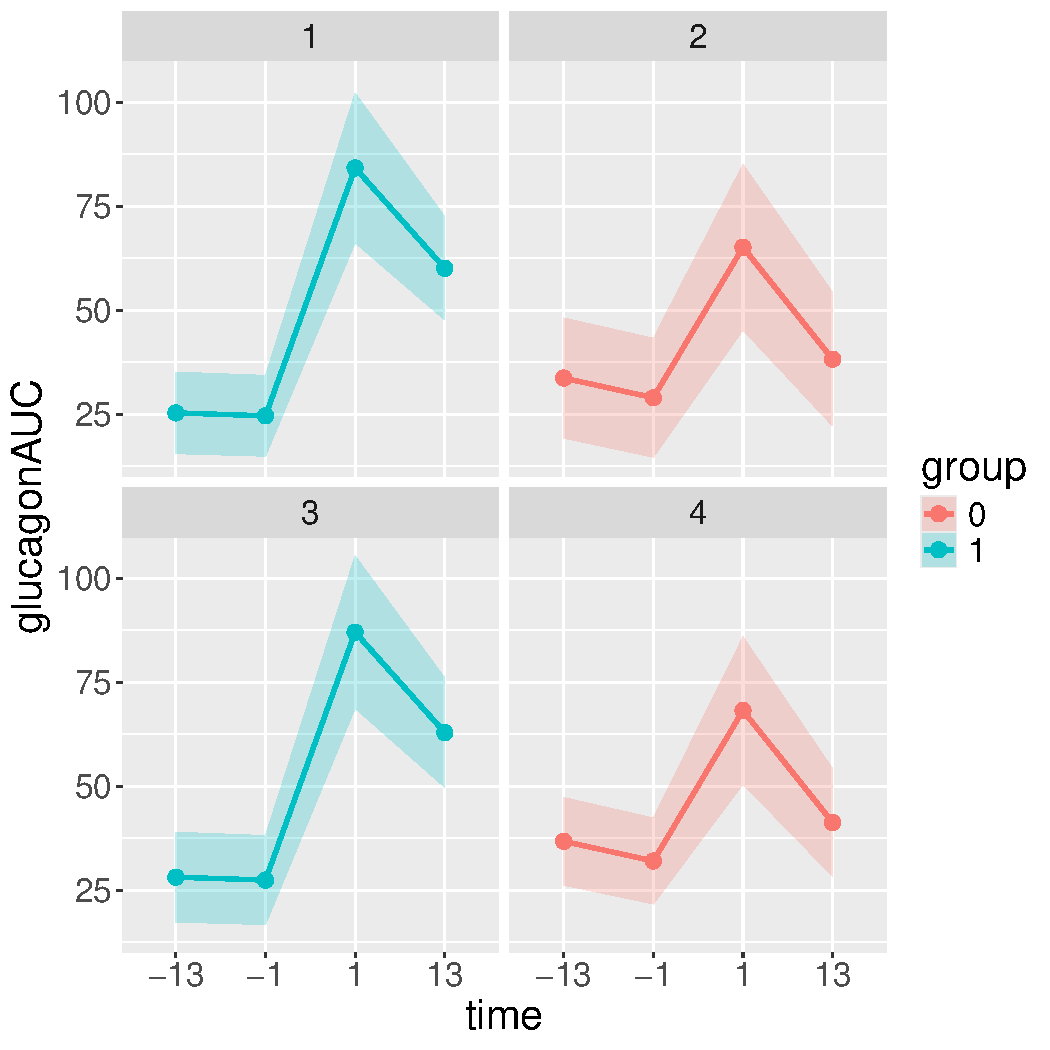
\includegraphics[width=\textwidth]{./figures/fit-autoplot-indiv.pdf}
\end{center}

\clearpage

\subsection{Partial residuals}
\label{sec:org63a7732}

Partial residuals can also be displayed via the \texttt{plot} method:
\lstset{language=r,label= ,caption= ,captionpos=b,numbers=none}
\begin{lstlisting}
gg1 <- plot(eUN.lmm, type = "partial", var = "glucagon")$plot
gg2 <- plot(eUN.lmm, type = "partial", var = c("(Intercept)","glucagon"))$plot
ggarrange(gg1,gg2)
\end{lstlisting}

\begin{center}
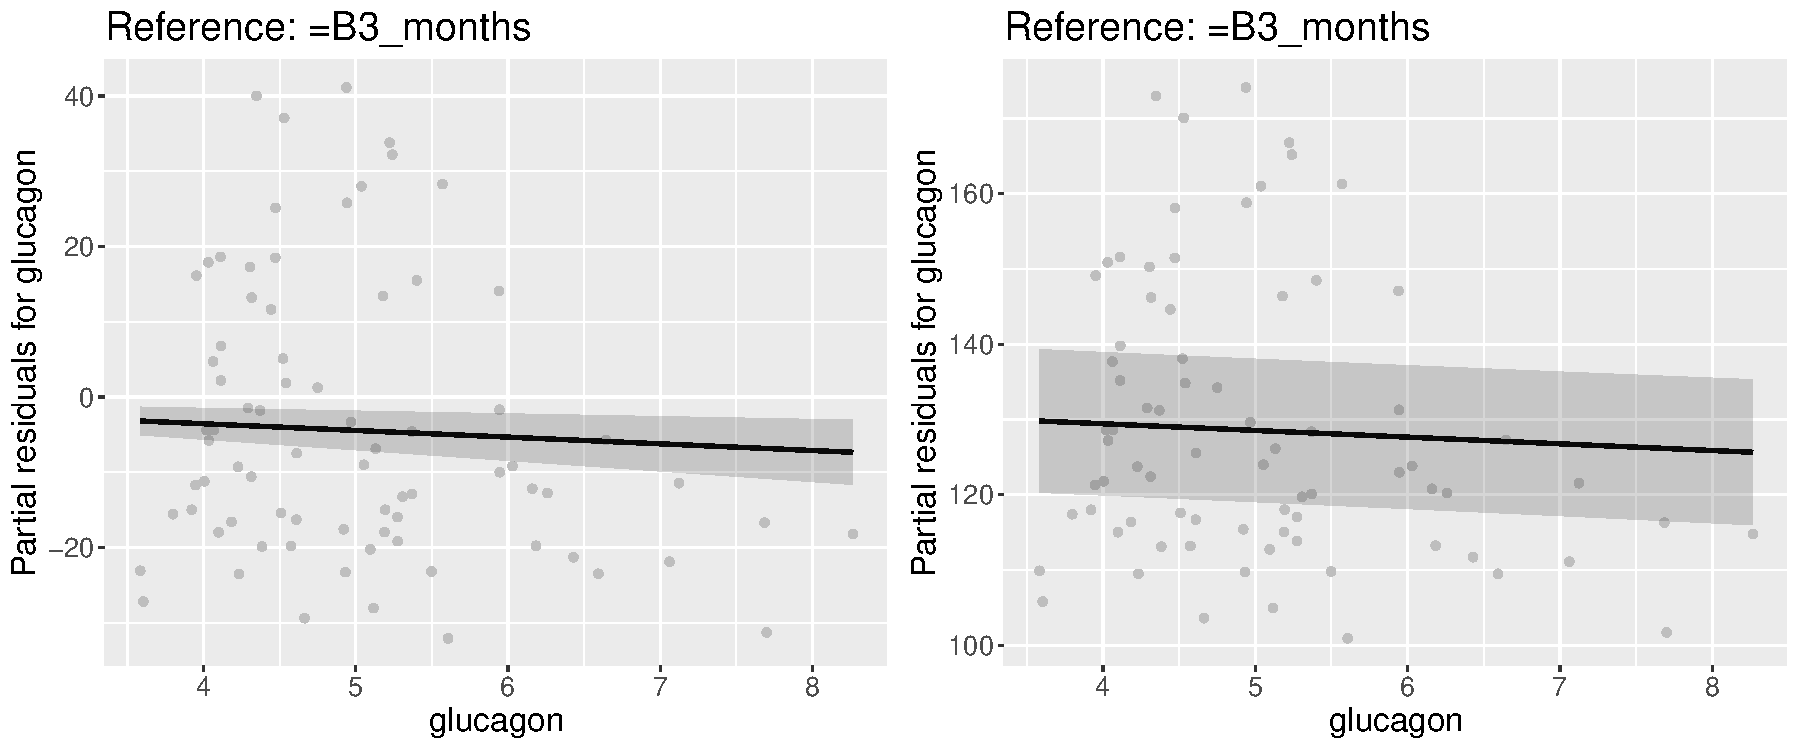
\includegraphics[width=0.75\textwidth]{./figures/fit-pres.pdf}
\end{center}

Their value can be extracted via the \texttt{residuals} method, e.g.:
\lstset{language=r,label= ,caption= ,captionpos=b,numbers=none}
\begin{lstlisting}
df.pres <- residuals(eUN.lmm, type = "partial", var = "glucagon", keep.data = TRUE)
head(df.pres)
\end{lstlisting}

\begin{verbatim}
  id visit time weight glucagonAUC baseline glucagon group    fitted  r.partial
1  1     1  B3m  127.2     5032.50     TRUE 4.034616     1 -3.583982  -5.780135
2  2     1  B3m  165.2    12142.50     TRUE 5.240766     0 -4.655415  32.219865
3  3     1  B3m  109.7    10321.35     TRUE 4.931824     1 -4.380979 -23.280135
4  4     1  B3m  146.2     6693.00     TRUE 4.316306     0 -3.834209  13.219865
5  5     1  B3m  113.1     7090.50     TRUE 4.383738     1 -3.894110 -19.880135
6  6     1  B3m  158.8    10386.00     TRUE 4.942791     0 -4.390721  25.819865
\end{verbatim}


This matches manual calculation:
\lstset{language=r,label= ,caption= ,captionpos=b,numbers=none}
\begin{lstlisting}
m.pres <- dfL$weight - model.matrix(~time,dfL) %*% coef(eUN.lmm)[1:4]
range(df.pres$r.partial - m.pres, na.rm = TRUE)

m.pfit <- model.matrix(~0+glucagon,dfL) %*% coef(eUN.lmm)["glucagon"]
range(df.pres$fitted - m.pfit, na.rm = TRUE)
\end{lstlisting}

\begin{verbatim}
[1] -1.065814e-14  1.421085e-14
[1] 0 0
\end{verbatim}


The \texttt{plot} methods can handle one continuous and one categorical
covariate (in addition to the intercept) to display interaction
plots. In that case each observation/fitted line is colored according
to the categorical covariate.

\clearpage

\subsection{Statistical inference (linear)}
\label{sec:org66e84f1}

The \texttt{anova} method can be use to test one or several linear
combinations of the model coefficients using Wald tests. By default,
it will simultaneously test all parameters associated to a variable:
\lstset{language=r,label= ,caption= ,captionpos=b,numbers=none}
\begin{lstlisting}
anova(eUN.lmm)
\end{lstlisting}

\begin{verbatim}
	     Multivariate Wald test 

               F-statistic       df  p.value    
mean: time          86.743 (3,19.0) 2.84e-11 ***
    : glucagon      13.518 (1,13.7)  0.00257  **
\end{verbatim}


Note that here the p-values are not adjust for multiple comparisons
over variables. It is possible to specify a null hypothesis to be
test: e.g. is there a change in average weight just after taking the
treatment:
\lstset{language=r,label= ,caption= ,captionpos=b,numbers=none}
\begin{lstlisting}
anova(eUN.lmm, effects = c("timeA1w-timeB1w=0"))
\end{lstlisting}

\begin{verbatim}
	     Multivariate Wald test 

       F-statistic       df  p.value    
all: 1      43.141 (1,17.9) 3.72e-06 ***
\end{verbatim}


One can also simulateneously tests several null hypotheses:
\lstset{language=r,label= ,caption= ,captionpos=b,numbers=none}
\begin{lstlisting}
e.anova <- anova(eUN.lmm, effects = c("timeA1w-timeB1w=0","timeA3m-timeB1w=0"))
summary(e.anova)
\end{lstlisting}

\begin{verbatim}
		Multivariate Wald test 

          F-statistic       df  p.value    
   all: 1      98.651 (2,18.6) 1.23e-10 ***
   ---------------------------------------- 
  Signif. codes:  0 '***' 0.001 '**' 0.01 '*' 0.05 '.' 0.1 ' ' 1.
  Degrees of freedom were computed using a Satterthwaite approximation (column df). 

		Univariate Wald test 

                     estimate    se   df   lower   upper p.value    
   timeA1w - timeB1w   -3.906 0.595 17.9  -5.325  -2.487   3e-05 ***
   timeA3m - timeB1w   -18.24 1.323   19 -21.397 -15.083  <1e-05 ***
   --------------------------------------------------------------- 
  Signif. codes:  0 '***' 0.001 '**' 0.01 '*' 0.05 '.' 0.1 ' ' 1.
  Columns lower/upper/p.value adjusted for multiple comparisons -- max-test.
  (1e+05 samples have been used)
  Model-based standard errors are derived from the observed information (column se). 
  Degrees of freedom were computed using a Satterthwaite approximation (column df).
\end{verbatim}

\clearpage

or return all pairwise comparisons for a given factor using the \texttt{mcp}
function of the multcomp package:
\lstset{language=r,label= ,caption= ,captionpos=b,numbers=none}
\begin{lstlisting}
library(multcomp)
summary(anova(eUN.lmm, effects = mcp(time = "Tukey")))
\end{lstlisting}

\begin{verbatim}
Singular contrast matrix: contrasts "A1w - B1w" "A3m - B1w" "A3m - A1w" have been removed. 

		Multivariate Wald test 

             F-statistic       df  p.value    
   all: time      86.743 (3,19.0) 2.84e-11 ***
   ------------------------------------------- 
  Signif. codes:  0 '***' 0.001 '**' 0.01 '*' 0.05 '.' 0.1 ' ' 1.
  Degrees of freedom were computed using a Satterthwaite approximation (column df). 

		Univariate Wald test 

             estimate    se   df   lower   upper p.value    
   B1w - B3m   -7.882 0.713 19.2  -9.817  -5.947  <1e-05 ***
   A1w - B3m  -11.788 1.018 21.6 -14.549  -9.027  <1e-05 ***
   A3m - B3m  -26.122 1.656 18.8 -30.617 -21.628  <1e-05 ***
   A1w - B1w   -3.906 0.595 17.9  -5.519  -2.292  <1e-05 ***
   A3m - B1w   -18.24 1.323   19 -21.829 -14.651  <1e-05 ***
   A3m - A1w  -14.334 1.057 20.3 -17.201 -11.468  <1e-05 ***
   --------------------------------------------------------- 
  Signif. codes:  0 '***' 0.001 '**' 0.01 '*' 0.05 '.' 0.1 ' ' 1.
  Columns lower/upper/p.value adjusted for multiple comparisons -- max-test.
  (1e+05 samples have been used)
  Model-based standard errors are derived from the observed information (column se). 
  Degrees of freedom were computed using a Satterthwaite approximation (column df).
\end{verbatim}

Here the \texttt{summary} method prints not only the global test but also the
result associated to each hypothesis. When testing transformed
variance or correlation parameters, parentheses (as in \texttt{log(k).B1w})
cause problem for recognizing parameters:
\lstset{language=r,label= ,caption= ,captionpos=b,numbers=none}
\begin{lstlisting}
try(
  anova(eUN.lmm,
        effects = c("log(k).B1w=0","log(k).A1w=0","log(k).A3m=0"))
)
\end{lstlisting}

\begin{verbatim}
Error in .anova_Wald(object, effects = effects, robust = robust, rhs = rhs,  : 
  Possible mispecification of the argument 'effects' as running mulcomp::glht lead to the following error: 
Error in parse(text = ex[i]) : <text>:1:7: uventet symbol
1: log(k).B1w
          ^
\end{verbatim}


\clearpage

It is then advised to build a contrast matrix, e.g.:
\lstset{language=r,label= ,caption= ,captionpos=b,numbers=none}
\begin{lstlisting}
name.coef <- rownames(confint(eUN.lmm, effects = "all"))
name.varcoef <- grep("^k",name.coef, value = TRUE)
C <- matrix(0, nrow = 3, ncol = length(name.coef), dimnames = list(name.varcoef, name.coef))
diag(C[name.varcoef,name.varcoef]) <- 1
C[,1:9]
\end{lstlisting}

\begin{verbatim}
      (Intercept) timeB1w timeA1w timeA3m glucagon sigma k.B1w k.A1w k.A3m
k.B1w           0       0       0       0        0     0     1     0     0
k.A1w           0       0       0       0        0     0     0     1     0
k.A3m           0       0       0       0        0     0     0     0     1
\end{verbatim}


And then call the \texttt{anova} method specifying the null hypothesis via the
contrast matrix:
\lstset{language=r,label= ,caption= ,captionpos=b,numbers=none}
\begin{lstlisting}
anova(eUN.lmm, effects = C)
\end{lstlisting}

\begin{verbatim}
	     Multivariate Wald test 

       F-statistic       df p.value   
all: 1       6.203 (3,18.0) 0.00442 **
\end{verbatim}


Note that using the approach of \cite{pipper2012versatile} it is also
possible to adjust for multiple testing across several \texttt{lmm}
objects. To do so, one first fit the mixed models, then use the
\texttt{anova} method to indicate which hypotheses are being tested, and
combine them using \texttt{rbind}. Here is an (artificial) example:
\lstset{language=r,label= ,caption= ,captionpos=b,numbers=none}
\begin{lstlisting}
Manova <- rbind(anova(eInd.lmm, effects = "glucagon = 0", robust = FALSE),
                anova(eCS.lmm, effects = "glucagon = 0", robust = FALSE),
                anova(eUN.lmm, effects = "glucagon = 0", robust = FALSE),
                name = c("Ind","CS","UN"))
summary(Manova) 
\end{lstlisting}

\begin{verbatim}
		Multivariate Wald test 

          Chi2-statistic      df  p.value    
   all: 1          8.893 (3,Inf) 6.88e-06 ***
   ------------------------------------------ 
  Signif. codes:  0 '***' 0.001 '**' 0.01 '*' 0.05 '.' 0.1 ' ' 1.

		Univariate Wald test 

                 estimate    se   df   lower  upper  p.value    
   Ind: glucagon    -8.27 2.579 34.2 -14.414 -2.126 0.003988  **
   CS: glucagon     0.822  0.62 53.8  -0.655  2.299 0.450012    
   UN: glucagon    -0.888 0.242 13.7  -1.464 -0.313 0.000711 ***
   ------------------------------------------------------------ 
  Signif. codes:  0 '***' 0.001 '**' 0.01 '*' 0.05 '.' 0.1 ' ' 1.
  Columns lower/upper/p.value adjusted for multiple comparisons -- max-test.
  (error when computing the adjusted columns lower/upper/p.value by numerical integration: 1.52e-05)
  Model-based standard errors are derived from the observed information (column se).
\end{verbatim}

\clearpage

\subsection{Statistical inference (non-linear)}
\label{sec:org23e784e}

The \texttt{estimate} function can be used to test one or several non-linear
combinations of model coefficients, using a first order delta method
to quantify uncertainty. The combination has to be specified via a
function (argument \texttt{f}). To illustrate its use consider an ANCOVA
analysis:
\[ Y_{i1} = \textcolor{\darkred}{\alpha} + \textcolor{\darkblue}{\beta} Y_{i,0} + \textcolor{\darkgreen}{\gamma} X_{i} + e_{i} \]

\lstset{language=r,label= ,caption= ,captionpos=b,numbers=none}
\begin{lstlisting}
e.ANCOVA <- lm(weight4 ~ weight1 + group, data = gastricbypassW)
summary(e.ANCOVA)$coef
\end{lstlisting}

\begin{verbatim}
              Estimate Std. Error    t value     Pr(>|t|)
(Intercept) -5.9285136 8.78006389 -0.6752244 5.086140e-01
weight1      0.8236279 0.06411563 12.8459772 3.524665e-10
group        4.1404554 2.53335466  1.6343765 1.205604e-01
\end{verbatim}


We can replicate this analysis by first fitting a mixed model:
\[ Y_{ij} = \alpha_j + \gamma_j X_{i} + \varepsilon_{i,j} \text{ where } \varepsilon_i \sim \Gaus \left( \begin{bmatrix} 0 \\ 0 \end{bmatrix}, \begin{bmatrix} \sigma^2_1 & \rho \sigma_1 \sigma_2 \\ \rho \sigma_1 \sigma_2 & \sigma^2_2 \end{bmatrix} \right) \]
\lstset{language=r,label= ,caption= ,captionpos=b,numbers=none}
\begin{lstlisting}
dfL14 <- dfL[dfL$visit %in% c(1,4),]
dfL14$time <- droplevels(dfL14$time)
e.lmmANCOVA <- lmm(weight ~ time+time:group, repetition = ~time|id,
                   data = dfL14)
\end{lstlisting}

and then perform a first order delta-method:
\lstset{language=r,label= ,caption= ,captionpos=b,numbers=none}
\begin{lstlisting}
lava::estimate(e.lmmANCOVA, f = function(p){
  c(Y1 = as.double(p["rho(B3m,A3m)"]*p["k.A3m"]),
    X1 = as.double(p["timeA3m:group"]-p["rho(B3m,A3m)"]*p["k.A3m"]*p["timeB3m:group"]))
})
\end{lstlisting}

\begin{verbatim}
    estimate         se        df      lower     upper      p.value
Y1 0.8236279 0.06230919  9.874633  0.6845551 0.9627007 1.332743e-07
X1 4.1404554 2.46197819 15.161269 -1.1022695 9.3831803 1.130927e-01
\end{verbatim}


Indeed:
\begin{align*}
\Esp[Y_{i2}|Y_{i1},X_{i}] &= \alpha_2 + \gamma_2 X_{i} + \rho \frac{\sigma_2}{\sigma_1}\left(Y_{i1} - \alpha_1 - \gamma_1 X_{i}\right) \\
                         &= \textcolor{\darkred}{\alpha_2 - \rho \frac{\sigma_2}{\sigma_1} \alpha_1}
                         + \textcolor{\darkblue}{\rho \frac{\sigma_2}{\sigma_1}Y_{i1}}
                         + \textcolor{\darkgreen}{\left(\gamma_2 - \rho \frac{\sigma_2}{\sigma_1} \gamma_1\right)  X_{i} }
\end{align*}

We obtain identical estimate but different standard-errors/degrees of
freedom compared to the univariate linear model approach. The later is
to be prefer as it does not rely on approximation. The former is
nevertheless useful as it can handle missing data in the outcome
variable.

\clearpage

\subsection{Baseline adjustment}
\label{sec:org90d3154}

In clinical trial the group and intervention variable often do not
coincide, e.g., in presence of baseline measurement. In our running
example, the first two measurement are pre-treatment (i.e. treatment
should be \texttt{"none"}) while the last two measurements are post-treatment
(i.e. treatment should be \texttt{1} or \texttt{2}). The \texttt{baselineAdjustment}
function can be helpful to:
\begin{itemize}
\item define the treatment variable from the time and allocation variable, where baseline has its specific value
\end{itemize}
\lstset{language=r,label= ,caption= ,captionpos=b,numbers=none}
\begin{lstlisting}
gastricbypassL$treat <- baselineAdjustment(gastricbypassL, variable = "group",
                                repetition = ~time|id, constrain = c("B3m","B1w"),
                                new.level = "none")
table(treat = gastricbypassL$treat, time = gastricbypassL$time, group = gastricbypassL$group)
\end{lstlisting}

\begin{verbatim}
, , group = 0

      time
treat  B3m B1w A1w A3m
  none  10  10   0   0
  0      0   0  10  10
  1      0   0   0   0

, , group = 1

      time
treat  B3m B1w A1w A3m
  none  10  10   0   0
  0      0   0   0   0
  1      0   0  10  10
\end{verbatim}

\begin{itemize}
\item define the treatment variable from the time and allocation variable,
where baseline corresponds to the reference group
\end{itemize}
\lstset{language=r,label= ,caption= ,captionpos=b,numbers=none}
\begin{lstlisting}
gastricbypassL$treat2 <- baselineAdjustment(gastricbypassL, variable = "group",
                                            repetition = ~time|id, constrain = c("B3m","B1w"))
table(treat = gastricbypassL$treat2, time = gastricbypassL$time, group = gastricbypassL$group)
\end{lstlisting}

\begin{verbatim}
, , group = 0

     time
treat B3m B1w A1w A3m
    1  10  10   0   0
    0   0   0  10  10

, , group = 1

     time
treat B3m B1w A1w A3m
    1  10  10  10  10
    0   0   0   0   0
\end{verbatim}

\begin{itemize}
\item define a time varying treatment variable from the time and allocation variable
\end{itemize}
\lstset{language=r,label= ,caption= ,captionpos=b,numbers=none}
\begin{lstlisting}
gastricbypassL$timeXtreat <- baselineAdjustment(gastricbypassL, variable = "group",
                                                repetition = ~time|id, constrain = c("B3m","B1w"),
                                                collapse.time = ".")

table(treat = gastricbypassL$timeXtreat, time = gastricbypassL$time, group = gastricbypassL$group)
\end{lstlisting}

\begin{verbatim}
, , group = 0

       time
treat   B3m B1w A1w A3m
  B3m    10   0   0   0
  B1w     0  10   0   0
  A1w.0   0   0  10   0
  A3m.0   0   0   0  10
  A1w.1   0   0   0   0
  A3m.1   0   0   0   0

, , group = 1

       time
treat   B3m B1w A1w A3m
  B3m    10   0   0   0
  B1w     0  10   0   0
  A1w.0   0   0   0   0
  A3m.0   0   0   0   0
  A1w.1   0   0  10   0
  A3m.1   0   0   0  10
\end{verbatim}

We would then typically like to model group differences only after
baseline (i.e. only at 1 week and 3 months after). This can be
performed using the time varying treatment variable, e.g.:
\lstset{language=r,label= ,caption= ,captionpos=b,numbers=none}
\begin{lstlisting}
eC.lmm <- lmm(weight ~ timeXtreat, data = gastricbypassL,
              repetition = ~time|id, structure = "UN")
coef(eC.lmm) ## change from baseline
\end{lstlisting}

\begin{verbatim}
(Intercept)   timeXtreatB1w timeXtreatA1w.0 timeXtreatA3m.0 timeXtreatA1w.1 timeXtreatA3m.1 
  128.97000        -7.73000       -13.38978       -28.52130       -13.15022       -24.68870
\end{verbatim}


or
\lstset{language=r,label= ,caption= ,captionpos=b,numbers=none}
\begin{lstlisting}
eC2.lmm <- lmm(weight ~ 0 + timeXtreat, data = gastricbypassL,
              repetition = ~time|id, structure = "UN")
coef(eC2.lmm) ## absolute value
\end{lstlisting}

\begin{verbatim}
timeXtreatB3m   timeXtreatB1w timeXtreatA1w.0 timeXtreatA3m.0 timeXtreatA1w.1 timeXtreatA3m.1 
     128.9700        121.2400        115.5802        100.4487        115.8198        104.2813
\end{verbatim}


The parametrization however does not (directly) output treatment
effects. Instead one may be tempted to use a formula like
\texttt{treatment*time}. However this will lead to a non-indentifiable
model. Indeed we are only able to estimate a total of 6 means when
constraining the expected baseline value between the two groups to be
the same. Therefore can at most identify 6 effects. However the design
matrix for the interaction model:
\lstset{language=r,label= ,caption= ,captionpos=b,numbers=none}
\begin{lstlisting}
colnames(model.matrix(weight ~ treat*time, data = gastricbypassL))
\end{lstlisting}

\begin{verbatim}
 [1] "(Intercept)"    "treat0"         "treat1"         "timeB1w"        "timeA1w"       
 [6] "timeA3m"        "treat0:timeB1w" "treat1:timeB1w" "treat0:timeA1w" "treat1:timeA1w"
[11] "treat0:timeA3m" "treat1:timeA3m"
\end{verbatim}


contains 12 parameters (i.e. 6 too many). Fortunately, the \texttt{lmm} will
 drop non-identifiable effects from the model and fit the resulting
 simplified model:
\lstset{language=r,label= ,caption= ,captionpos=b,numbers=none}
\begin{lstlisting}
eC3.lmm <- lmm(weight ~ treat2*time, data = gastricbypassL,
               repetition = ~time|id, structure = "UN")
\end{lstlisting}

\begin{verbatim}
Constant values in the design matrix for the mean structure.
Coefficients "treat20" "treat20:timeB1w" relative to interactions "treat2:time" have been removed.
\end{verbatim}


with the following coefficients:
\lstset{language=r,label= ,caption= ,captionpos=b,numbers=none}
\begin{lstlisting}
model.tables(eC3.lmm)
\end{lstlisting}

\begin{verbatim}
                   estimate        se       df      lower       upper      p.value
(Intercept)     128.9700000 4.5323695 18.98130 119.483009 138.4569912 0.000000e+00
timeB1w          -7.7300000 0.6974427 18.97552  -9.189892  -6.2701082 9.938186e-10
timeA1w         -13.1502219 0.8970429 22.87334 -15.006465 -11.2939786 4.058975e-13
timeA3m         -24.6886957 1.7751662 22.25061 -28.367762 -21.0096290 1.863398e-12
treat20:timeA1w  -0.2395562 0.6484895 17.66860  -1.603816   1.1247037 7.162149e-01
treat20:timeA3m  -3.8326086 2.1066817 17.60613  -8.265691   0.6004734 8.592047e-02
\end{verbatim}


One can vizualize the baseline adjustment via the \texttt{plot} function:
\lstset{language=r,label= ,caption= ,captionpos=b,numbers=none}
\begin{lstlisting}
plot(eC3.lmm, color = "group", ci = FALSE, size.text = 20, obs.alpha = 0.1)
\end{lstlisting}

\begin{center}
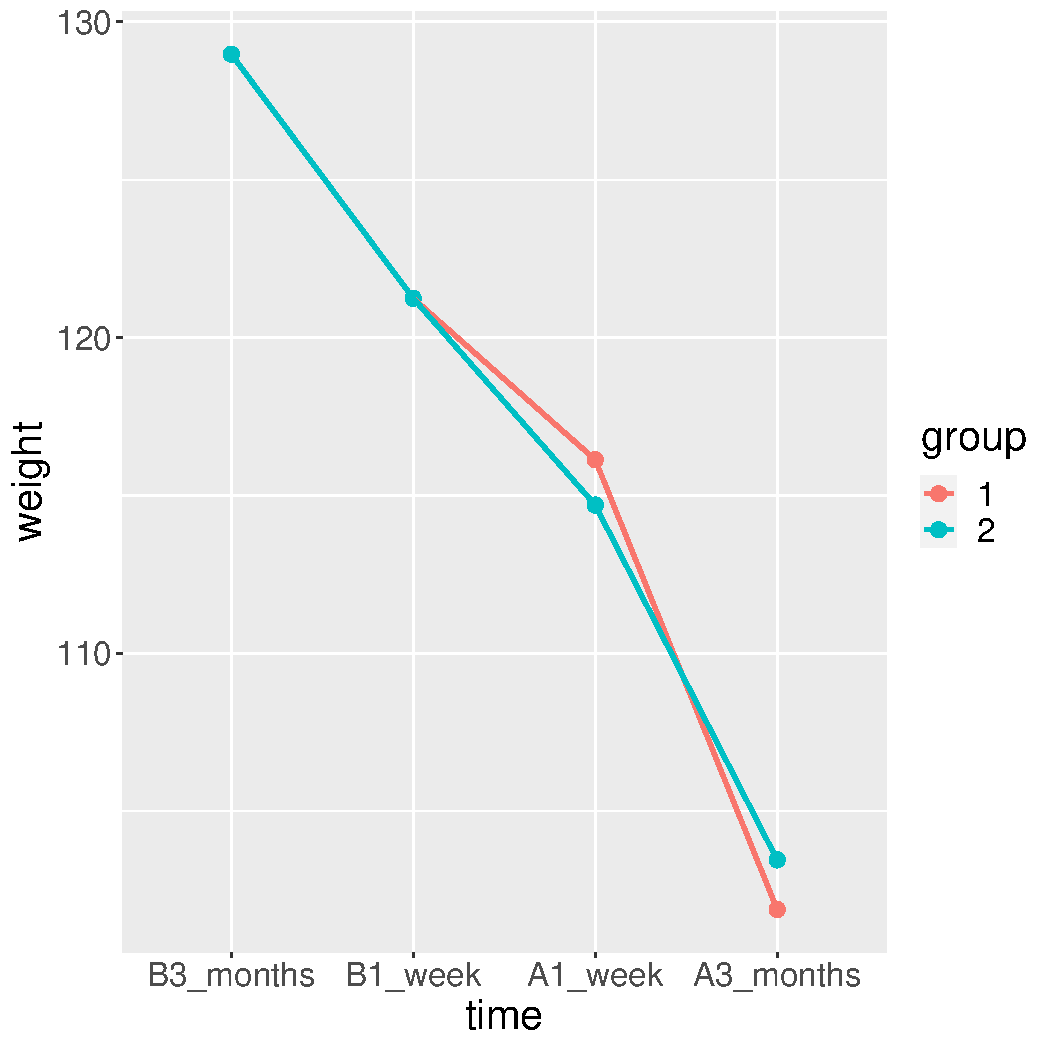
\includegraphics[width=0.4\textwidth]{./figures/gg-baseAdj.pdf}
\end{center}

\subsection{Marginal means}
\label{sec:org732ecba}

The \texttt{emmeans} package can be used to output marginal means. Consider
the following model:
\lstset{language=r,label= ,caption= ,captionpos=b,numbers=none}
\begin{lstlisting}
dfL$group2 <- as.numeric(dfL$id) %% 3 == 0
e.group <- lmm(glucagon ~ time*group2, data = dfL,
               repetition = ~time|id, structure = "UN")
\end{lstlisting}

We can for instance compute the average value over time \emph{assuming balanced groups}:
\lstset{language=r,label= ,caption= ,captionpos=b,numbers=none}
\begin{lstlisting}
emmeans(e.group, specs=~time)
\end{lstlisting}

\begin{verbatim}
NOTE: Results may be misleading due to involvement in interactions
 time emmean    SE   df lower.CL upper.CL
 B3m    4.45 0.156 18.0     4.12     4.78
 B1w    4.32 0.131 18.0     4.05     4.60
 A1w    5.95 0.262 18.4     5.40     6.50
 A3m    5.12 0.187 18.0     4.73     5.51

Results are averaged over the levels of: group2 
Confidence level used: 0.95
\end{verbatim}


This differs from the average value over time over the whole sample:
\lstset{language=r,label= ,caption= ,captionpos=b,numbers=none}
\begin{lstlisting}
df.pred <- predict(e.group, newdata = dfL, keep.newdata = TRUE)
summarize(formula = estimate~time, data = df.pred)
\end{lstlisting}

\begin{verbatim}
  time observed missing     mean        sd      min       q1   median       q3      max
1  B3m       20       0 4.514352 0.1502565 4.290643 4.290643 4.610227 4.610227 4.610227
2  B1w       19       0 4.384638 0.1643256 4.149209 4.149209 4.493298 4.493298 4.493298
3  A1w       19       0 6.060587 0.2030012 5.729961 5.954314 6.178668 6.178668 6.178668
4  A3m       20       0 5.057642 0.1465315 4.964144 4.964144 4.964144 5.275805 5.275805
\end{verbatim}


as the groups are not balanced:
\lstset{language=r,label= ,caption= ,captionpos=b,numbers=none}
\begin{lstlisting}
table(group = dfL$group2, time = dfL$time)
\end{lstlisting}

\begin{verbatim}
       time
group   B3m B1w A1w A3m
  FALSE  14  13  14  14
  TRUE    6   6   5   6
\end{verbatim}


The "emmeans" approach gives equal "weight" to the expected value of
both group:
\lstset{language=r,label= ,caption= ,captionpos=b,numbers=none}
\begin{lstlisting}
mu.group1 <-  as.double(coef(e.group)["(Intercept)"])
mu.group2 <-  as.double(coef(e.group)["(Intercept)"] + coef(e.group)["group2TRUE"])
p.group1 <- 14/20          ; p.group2 <- 6/20
c(emmeans = (mu.group1+mu.group2)/2, predict = mu.group1 * p.group1 + mu.group2 * p.group2)
\end{lstlisting}

\begin{verbatim}
 emmeans  predict 
4.450435 4.514352
\end{verbatim}


Which one is relevant depends on the application. The \texttt{emmeans}
function can also be used to display expected value in each group over
time:
\lstset{language=r,label= ,caption= ,captionpos=b,numbers=none}
\begin{lstlisting}
emmeans.group <- emmeans(e.group, specs = ~group2|time)
emmeans.group
\end{lstlisting}

\begin{verbatim}
time = B3m:
 group2 emmean    SE   df lower.CL upper.CL
 FALSE    4.61 0.171 18.0     4.25     4.97
  TRUE    4.29 0.262 18.0     3.74     4.84

time = B1w:
 group2 emmean    SE   df lower.CL upper.CL
 FALSE    4.49 0.145 18.4     4.19     4.80
  TRUE    4.15 0.219 17.9     3.69     4.61

time = A1w:
 group2 emmean    SE   df lower.CL upper.CL
 FALSE    6.18 0.277 17.8     5.60     6.76
  TRUE    5.73 0.446 18.6     4.80     6.66

time = A3m:
 group2 emmean    SE   df lower.CL upper.CL
 FALSE    4.96 0.205 18.0     4.53     5.39
  TRUE    5.28 0.313 18.0     4.62     5.93

Confidence level used: 0.95
\end{verbatim}

\clearpage

Using the \texttt{pair} function displays the differences:
\lstset{language=r,label= ,caption= ,captionpos=b,numbers=none}
\begin{lstlisting}
epairs.group <- pairs(emmeans.group, reverse = TRUE)
epairs.group
\end{lstlisting}

\begin{verbatim}
time = B3m:
 contrast     estimate    SE   df t.ratio p.value
 TRUE - FALSE   -0.320 0.313 18.0  -1.022  0.3202

time = B1w:
 contrast     estimate    SE   df t.ratio p.value
 TRUE - FALSE   -0.344 0.262 18.0  -1.311  0.2062

time = A1w:
 contrast     estimate    SE   df t.ratio p.value
 TRUE - FALSE   -0.449 0.525 18.4  -0.855  0.4034

time = A3m:
 contrast     estimate    SE   df t.ratio p.value
 TRUE - FALSE    0.312 0.374 18.0   0.834  0.4153
\end{verbatim}

One can adjust for multiple comparison via the \texttt{adjust} argument and
display confidence intervals setting the argument \texttt{infer} to \texttt{TRUE}:
\lstset{language=r,label= ,caption= ,captionpos=b,numbers=none}
\begin{lstlisting}
summary(epairs.group, by = NULL, adjust = "mvt", infer = TRUE)
\end{lstlisting}

\begin{verbatim}
 contrast     time estimate    SE   df lower.CL upper.CL t.ratio p.value
 TRUE - FALSE B3m    -0.320 0.313 18.0   -1.156    0.517  -1.022  0.6926
 TRUE - FALSE B1w    -0.344 0.262 18.0   -1.046    0.358  -1.311  0.5061
 TRUE - FALSE A1w    -0.449 0.525 18.4   -1.853    0.955  -0.855  0.7960
 TRUE - FALSE A3m     0.312 0.374 18.0   -0.689    1.312   0.834  0.8084

Confidence level used: 0.95 
Conf-level adjustment: mvt method for 4 estimates 
P value adjustment: mvt method for 4 tests
\end{verbatim}


This should also work when doing baseline adjustment (because of
baseline adjustment no difference is expected at the first two
timepoints):
\lstset{language=r,label= ,caption= ,captionpos=b,numbers=none}
\begin{lstlisting}
summary(pairs(emmeans(eC3.lmm , specs = ~treat2|time), reverse = TRUE), by = NULL)
\end{lstlisting}

\begin{verbatim}
Note: adjust = "tukey" was changed to "sidak"
because "tukey" is only appropriate for one set of pairwise comparisons
 contrast          time estimate    SE  df t.ratio p.value
 treat20 - treat21 B3m      0.00 0.000 Inf     NaN     NaN
 treat20 - treat21 B1w      0.00 0.000 Inf     NaN     NaN
 treat20 - treat21 A1w     -0.24 0.648  18  -0.369  0.9195
 treat20 - treat21 A3m     -3.83 2.107  18  -1.819  0.1645

P value adjustment: sidak method for 2 tests
\end{verbatim}


\clearpage

\subsection{Predictions}
\label{sec:orgdbee46f}

Two types of predictions can be performed with the \texttt{predict} method:
\begin{itemize}
\item \textbf{static predictions} that are only conditional on the covariates:
\end{itemize}
\lstset{language=r,label= ,caption= ,captionpos=b,numbers=none}
\begin{lstlisting}
news <- dfL[dfL$id==1,]
news$glucagon <- 0
predict(eUN.lmm, newdata = news)
\end{lstlisting}

\begin{verbatim}
  estimate       se       df     lower    upper
1 132.9801 4.664247 19.75815 123.24305 142.7172
2 125.0979 4.388294 19.91418 115.94155 134.2543
3 121.1922 4.214230 20.55331 112.41660 129.9678
4 106.8577 3.942058 20.95499  98.65871 115.0568
\end{verbatim}


which can be computing by creating a design matrix:
\lstset{language=r,label= ,caption= ,captionpos=b,numbers=none}
\begin{lstlisting}
X.12 <- model.matrix(formula(eUN.lmm), news)
X.12
\end{lstlisting}

\begin{verbatim}
   (Intercept) timeB1w timeA1w timeA3m glucagon
1            1       0       0       0        0
21           1       1       0       0        0
41           1       0       1       0        0
61           1       0       0       1        0
attr(,"assign")
[1] 0 1 1 1 2
attr(,"contrasts")
attr(,"contrasts")$time
[1] "contr.treatment"
\end{verbatim}

and then multiplying it with the regression coefficients:
\lstset{language=r,label= ,caption= ,captionpos=b,numbers=none}
\begin{lstlisting}
X.12 %*% coef(eUN.lmm)
\end{lstlisting}

\begin{verbatim}
       [,1]
1  132.9801
21 125.0979
41 121.1922
61 106.8577
\end{verbatim}


\clearpage

\begin{itemize}
\item \textbf{dynamic predictions} that are conditional on the covariates and the
outcome measured at other timepoints. Consider two subjects for who
we would like to predict the weight 1 week before the intervention
based on the weight 3 months before the intervention:
\end{itemize}

\lstset{language=r,label= ,caption= ,captionpos=b,numbers=none,otherkeywords={}, deletekeywords={}}
\begin{lstlisting}
newd <- rbind(
  data.frame(id = 1, time = "B3m", weight = coef(eUN.lmm)["(Intercept)"], glucagon = 0),
  data.frame(id = 1, time = "B1w", weight = NA, glucagon = 0),
  data.frame(id = 2, time = "B3m", weight = 100, glucagon = 0),
  data.frame(id = 2, time = "B1w", weight = NA, glucagon = 0)
)
predict(eUN.lmm, newdata = newd, type = "dynamic", keep.newdata = TRUE)
\end{lstlisting}

\begin{verbatim}
  id time   weight glucagon  estimate        se  df     lower    upper
1  1  B3m 132.9801        0        NA        NA Inf        NA       NA
2  1  B1w       NA        0 125.09790 0.6362754 Inf 123.85083 126.3450
3  2  B3m 100.0000        0        NA        NA Inf        NA       NA
4  2  B1w       NA        0  94.47017 7.2279385 Inf  80.30367 108.6367
\end{verbatim}


The first subjects has the average weight while the second has a much
  lower weight. The predicted weight for the first subject is then the
  average weight one week before while it is lower for the second
  subject due to the positive correlation over time. The predicted
  value is computed using the formula of the conditional mean for a
  Gaussian vector:
\lstset{language=r,label= ,caption= ,captionpos=b,numbers=none}
\begin{lstlisting}
mu1 <- coef(eUN.lmm)[1]
mu2 <- sum(coef(eUN.lmm)[1:2])
Omega_11 <- sigma(eUN.lmm)["B3m","B3m"]
Omega_21 <- sigma(eUN.lmm)["B1w","B3m"]
as.double(mu2 + Omega_21 * (100 - mu1) / Omega_11)
\end{lstlisting}

\begin{verbatim}
[1] 94.47017
\end{verbatim}



\clearpage

\section{Equivalence with other statistical methods}
\label{sec:org6f3eff7}
\subsection{T-test}
\label{sec:org5d9b2ee}
A t-test:
\lstset{language=r,label= ,caption= ,captionpos=b,numbers=none}
\begin{lstlisting}
t.test(weight4 ~ group, data = gastricbypassW)
\end{lstlisting}

\begin{verbatim}

	Welch Two Sample t-test

data:  weight4 by group
t = 0.59144, df = 17.679, p-value = 0.5617
alternative hypothesis: true difference in means between group 0 and group 1 is not equal to 0
95 percent confidence interval:
 -11.73582  20.91582
sample estimates:
mean in group 0 mean in group 1 
         104.66          100.07
\end{verbatim}

is equivalent to an independent covariance pattern with a different
variable for each group:
\lstset{language=r,label= ,caption= ,captionpos=b,numbers=none}
\begin{lstlisting}
e.ttest4 <- lmm(weight4 ~ group, structure = IND(~group), 
               data = gastricbypassW, trace = FALSE)
model.tables(e.ttest4)
\end{lstlisting}

\begin{verbatim}
            estimate       se       df     lower     upper      p.value
(Intercept)   104.66 5.104469  9.00180  93.11324 116.20676 7.270954e-09
group          -4.59 7.760674 17.68244 -20.91558  11.73558 5.617090e-01
\end{verbatim}


Multiple t-tests:
\lstset{language=r,label= ,caption= ,captionpos=b,numbers=none}
\begin{lstlisting}
e.ttest1 <- lmm(weight1 ~ group, structure = IND(~group), 
                data = gastricbypassW, trace = FALSE)
e.ttest2 <- lmm(weight2 ~ group, structure = IND(~group), 
                data = gastricbypassW, trace = FALSE)
e.ttest3 <- lmm(weight3 ~ group, structure = IND(~group), 
                data = gastricbypassW, trace = FALSE)
\end{lstlisting}

can be adjusted for multiple comparison by first using the \texttt{anova}
function to specify the parameter of interest and combining the
results using \texttt{rbind}:
\lstset{language=r,label= ,caption= ,captionpos=b,numbers=none}
\begin{lstlisting}
e.mttest <- rbind(anova(e.ttest1, effects = "group=0"),
                  anova(e.ttest2, effects = "group=0"),
                  anova(e.ttest3, effects = "group=0"),
                  anova(e.ttest4, effects = "group=0"))
model.tables(e.mttest, method = "bonferroni")
\end{lstlisting}

\begin{verbatim}
               estimate       se       df     lower    upper p.value
weight1: group   -10.60 8.971747 17.96464 -35.49775 14.29775       1
weight2: group    -9.50 8.395143 17.98540 -32.79464 13.79464       1
weight3: group    -8.92 8.129458 17.95876 -31.48110 13.64110       1
weight4: group    -4.59 7.760674 17.68244 -26.16472 16.98472       1
\end{verbatim}


\Warning efficient adjustment for multiple comparisons (like
\texttt{"single-step"}) will not be valid as the correlation structure has
not be specified. To do so it is more conveniently to work with a the
long format:
\lstset{language=r,label= ,caption= ,captionpos=b,numbers=none}
\begin{lstlisting}
e.mttest2 <- mlmm(weight ~ group, structure = IND(~group),
                  data = gastricbypassL, trace = FALSE,
                  effects = "group=0", by = "time", repetition = ~time|id)
model.tables(e.mttest2, method = "single-step2")
\end{lstlisting}

\begin{verbatim}
   by parameter estimate       se       df     lower     upper   p.value
1 B3m     group   -10.60 8.971747 17.96464 -30.90465  9.704648 0.3166268
2 B1w     group    -9.50 8.395143 17.98540 -28.49969  9.499691 0.3400966
3 A1w     group    -8.92 8.129458 17.95876 -27.31840  9.478400 0.3566864
4 A3m     group    -4.59 7.760674 17.68244 -22.15378 12.973775 0.6673833
\end{verbatim}


or call the dedicated function \texttt{mt.test}:
\lstset{language=r,label= ,caption= ,captionpos=b,numbers=none}
\begin{lstlisting}
mt.test(weight1+weight2+weight3+weight4~group, data = gastricbypassW)
\end{lstlisting}

\begin{verbatim}
       by parameter estimate       se       df     lower     upper   p.value
1 weight1     group   -10.60 8.971747 17.96464 -30.92628  9.726280 0.3200568
2 weight2     group    -9.50 8.395143 17.98540 -28.51993  9.519932 0.3433166
3 weight3     group    -8.92 8.129458 17.95876 -27.33800  9.498000 0.3602064
4 weight4     group    -4.59 7.760674 17.68244 -22.17249 12.992487 0.6654633
\end{verbatim}

\subsection{Linear regression on the change}
\label{sec:org1a1dba1}

A widely spread approach to analyze longitudinal data is to reduce the
number of repetitions to 1 by working on the change and then apply
'usual' statistical methods. For instance one could compare the pre-
and post- operation values using:

\lstset{language=r,label= ,caption= ,captionpos=b,numbers=none}
\begin{lstlisting}
gastricbypassW$changeG41 <- gastricbypassW$glucagonAUC4-gastricbypassW$glucagonAUC1
e.change41 <- lm(changeG41 ~ weight1, data = gastricbypassW)
summary(e.change41)$coef
\end{lstlisting}

\begin{verbatim}
             Estimate Std. Error   t value   Pr(>|t|)
(Intercept) 17865.953 9292.61106  1.922598 0.07050076
weight1      -113.696   71.22173 -1.596367 0.12781371
\end{verbatim}


\clearpage

This turns out to be equivalent to the following mixed model:
\lstset{language=r,label= ,caption= ,captionpos=b,numbers=none}
\begin{lstlisting}
gastricbypassL41 <- gastricbypassL[gastricbypassL$visit %in% c(1,4),]
gastricbypassL41$time <- droplevels(gastricbypassL41$time)
gastricbypassL41$weight1 <- gastricbypassW$weight1[gastricbypassL41$id]

e.lmm41 <- lmm(glucagonAUC ~ time + time*weight1,
               repetition =~ time|id, structure = "UN",
               data = gastricbypassL41)
model.tables(e.lmm41)
\end{lstlisting}

\begin{verbatim}
                    estimate         se       df       lower       upper    p.value
(Intercept)      7730.051990 5737.22268 18.00298 -4323.26268 19783.36666 0.19458155
timeA3m         17865.953183 9292.61106 18.00104 -1657.01749 37388.92385 0.07049983
weight1             1.011014   43.97202 18.00298   -91.36968    93.39171 0.98190941
timeA3m:weight1  -113.695981   71.22173 18.00104  -263.32666    35.93469 0.12781271
\end{verbatim}


This equivalence only holds as there is no missing data.
\lstset{language=r,label= ,caption= ,captionpos=b,numbers=none}
\begin{lstlisting}
index.missing41 <- which(is.na(gastricbypassW$changeG41))
index.missing41
\end{lstlisting}

\begin{verbatim}
integer(0)
\end{verbatim}

\subsection{Correlation between changes}
\label{sec:org83875a8}

In some studies, one is interested in studying the relation between
two evolutions. Say weight and glucagon before and after the
operation:
\lstset{language=r,label= ,caption= ,captionpos=b,numbers=none}
\begin{lstlisting}
gastricbypassW$changeG41 <- gastricbypassW$glucagonAUC4-gastricbypassW$glucagonAUC1
gastricbypassW$changeW41 <- gastricbypassW$weight4-gastricbypassW$weight1
\end{lstlisting}

\clearpage

One can evaluate their correlation:
\lstset{language=r,label= ,caption= ,captionpos=b,numbers=none}
\begin{lstlisting}
cor.test(gastricbypassW$changeW41, gastricbypassW$changeG41)
\end{lstlisting}

\begin{verbatim}

	Pearson's product-moment correlation

data:  gastricbypassW$changeW41 and gastricbypassW$changeG41
t = 1.8667, df = 18, p-value = 0.07831
alternative hypothesis: true correlation is not equal to 0
95 percent confidence interval:
 -0.0484149  0.7174011
sample estimates:
      cor 
0.4027343
\end{verbatim}

or regress one against the other:
\lstset{language=r,label= ,caption= ,captionpos=b,numbers=none}
\begin{lstlisting}
e2.change41 <- lm(changeG41 ~ changeW41, data = gastricbypassW)
summary(e2.change41)$coef
\end{lstlisting}

\begin{verbatim}
              Estimate Std. Error  t value   Pr(>|t|)
(Intercept) 13321.9427  5592.8058 2.381978 0.02845909
changeW41     380.3556   203.7541 1.866738 0.07831464
\end{verbatim}


This problem can be recast using all measurement as outcomes:
\lstset{language=r,label= ,caption= ,captionpos=b,numbers=none}
\begin{lstlisting}
keep.col <- c("id","weight1","weight4","glucagonAUC1","glucagonAUC4")
gastricbypassL4 <- reshape(gastricbypassW[,keep.col], direction = "long",
                           idvar = "id", varying = 2:5, timevar = "type", v.names = "value")
gastricbypassL4$type <- factor(gastricbypassL4$type, labels = keep.col[-1])
gastricbypassL4 <- gastricbypassL4[order(gastricbypassL4$id),]
head(gastricbypassL4)
\end{lstlisting}

\begin{verbatim}
    id         type   value
1.1  1      weight1  127.20
1.2  1      weight4  108.10
1.3  1 glucagonAUC1 5032.50
1.4  1 glucagonAUC4 9249.45
2.1  2      weight1  165.20
2.2  2      weight4  132.00
\end{verbatim}


fitting an unstructured mixed model:
\lstset{language=r,label= ,caption= ,captionpos=b,numbers=none}
\begin{lstlisting}
e.lmm4 <- lmm(value ~ type,
              repetition = ~type|id, structure = "UN",
              data = gastricbypassL4)
\end{lstlisting}

extract the residual covariance matrix:
\lstset{language=r,label= ,caption= ,captionpos=b,numbers=none}
\begin{lstlisting}
sigma.lmm4 <- sigma(e.lmm4)
sigma.lmm4
\end{lstlisting}

\begin{verbatim}
                 weight1     weight4  glucagonAUC1 glucagonAUC4
weight1         410.8475    326.8357      415.3727    -46296.33
weight4         326.8357    290.8350    -5983.5871    -34434.03
glucagonAUC1    415.3727  -5983.5871 14299430.9269  -4229230.69
glucagonAUC4 -46296.3339 -34434.0320 -4229230.6877  20065722.32
\end{verbatim}


Deduce the residual covariance matrix for the change:
\lstset{language=r,label= ,caption= ,captionpos=b,numbers=none}
\begin{lstlisting}
Mcon <- cbind(c(-1,1,0,0),c(0,0,-1,1))
sigmeChange.lmm4 <- t(Mcon) %*% sigma.lmm4 %*% Mcon
dimnames(sigmeChange.lmm4) <- list(c("d.weight","d.glucagonAUC"),
                                   c("d.weight","d.glucagonAUC"))
sigmeChange.lmm4
\end{lstlisting}

\begin{verbatim}
                 d.weight d.glucagonAUC
d.weight         48.01103      18261.26
d.glucagonAUC 18261.26175   42823614.62
\end{verbatim}


and the corrrelation or covariance:
\lstset{language=r,label= ,caption= ,captionpos=b,numbers=none}
\begin{lstlisting}
cov2cor(sigmeChange.lmm4)[1,2]
sigmeChange.lmm4[1,2]/sigmeChange.lmm4[1,1]
\end{lstlisting}

\begin{verbatim}
[1] 0.4027343
[1] 380.3556
\end{verbatim}


The uncertainty can be quantified using a delta method:
\lstset{language=r,label= ,caption= ,captionpos=b,numbers=none}
\begin{lstlisting}
estimate(e.lmm4, function(p){
  Sigma.change <- t(Mcon) %*% sigma(e.lmm4, p = p) %*% Mcon
  c(cor = cov2cor(Sigma.change)[1,2],
    beta = Sigma.change[1,2]/Sigma.change[1,1])
})
\end{lstlisting}

\begin{verbatim}
        estimate          se       df        lower       upper   p.value
cor    0.4027343   0.1922078 2.660595   -0.2555602    1.061029 0.1386265
beta 380.3555798 198.3453360 2.798661 -277.3518013 1038.062961 0.1575655
\end{verbatim}


The standard errors and degrees of freedom do not match the univariate
analysis, suggesting probably poor small sample properties of this
technic.

\clearpage

\section{Missing values and imputation}
\label{sec:org7479046}

We reconsider the example of the previous section, but now in presence
of missing values. The \texttt{summarize} function can be used to describe
the amount of missing data at each repetition:
\lstset{language=r,label= ,caption= ,captionpos=b,numbers=none}
\begin{lstlisting}
sss <- summarize(glucagon ~ time, data = gastricbypassL, na.rm = TRUE)
cbind(sss[,1:4], pc = paste0(100 * sss$missing / (sss$missing + sss$observed), "%"))
\end{lstlisting}

\begin{verbatim}
   outcome time observed missing pc
1 glucagon  B3m       20       0 0%
2 glucagon  B1w       19       1 5%
3 glucagon  A1w       19       1 5%
4 glucagon  A3m       20       0 0%
\end{verbatim}


For more detail about the missing data patters, see the \texttt{summarizeNA}
function:
\lstset{language=r,label= ,caption= ,captionpos=b,numbers=none}
\begin{lstlisting}
summarizeNA(data = gastricbypassL, repetition = ~ time|id)
\end{lstlisting}

\begin{verbatim}
    variable frequency missing.pattern n.missing id B3m B1w A1w A3m
       visit        20           00000         0  0   0   0   0   0
      weight        20           00000         0  0   0   0   0   0
 glucagonAUC        18           00000         0  0   0   0   0   0
                     1           00100         1  0   0   1   0   0
                     1           00010         1  0   0   0   1   0
    baseline        20           00000         0  0   0   0   0   0
    glucagon        18           00000         0  0   0   0   0   0
                     1           00100         1  0   0   1   0   0
                     1           00010         1  0   0   0   1   0
       group        20           00000         0  0   0   0   0   0
\end{verbatim}

To begin with we will only consider 1 week before and 1 week after
surgery:
\lstset{language=r,label= ,caption= ,captionpos=b,numbers=none}
\begin{lstlisting}
## long format
gastricbypassL32 <- gastricbypassL[gastricbypassL$visit %in% c(3,2),]
gastricbypassL32$time <- droplevels(gastricbypassL32$time)
gastricbypassL32$weight1 <- gastricbypassW$weight1[gastricbypassL32$id]
## wide format
gastricbypassW$changeG32 <- gastricbypassW$glucagonAUC3-gastricbypassW$glucagonAUC2
\end{lstlisting}

\clearpage

\subsection{Full information approach}
\label{sec:orgcba4a2c}

LMM uses a full information approach:
\lstset{language=r,label= ,caption= ,captionpos=b,numbers=none}
\begin{lstlisting}
e.lmm32 <- lmm(glucagonAUC ~ time + time*weight1,
               repetition =~ time|id, structure = "UN",
               data = gastricbypassL32)
model.tables(e.lmm32)
\end{lstlisting}

\begin{verbatim}
                   estimate         se       df       lower       upper      p.value
(Intercept)      2226.30678 4973.21491 17.01148 -8265.72037 12718.33393 0.6600471546
timeA1w         37469.89400 8950.26818 17.88948 18657.74792 56282.04008 0.0005612515
weight1            37.90933   37.87004 17.01113   -41.98548   117.80414 0.3308362562
timeA1w:weight1  -213.20181   68.15807 17.71309  -356.56304   -69.84058 0.0058968630
\end{verbatim}


whereas a linear model would perform a complete case approach:
\lstset{language=r,label= ,caption= ,captionpos=b,numbers=none}
\begin{lstlisting}
e.change32 <- lm(changeG32 ~ weight1, data = gastricbypassW)
summary(e.change32)$coef
\end{lstlisting}

\begin{verbatim}
              Estimate Std. Error   t value     Pr(>|t|)
(Intercept) 38101.9400 9417.61506  4.045816 0.0009373023
weight1      -217.2672   71.25218 -3.049271 0.0076504030
\end{verbatim}


In the former the likelihood is evaluated using all observations, even
those from individuals with some (but not all) missing outcome values:
baseline is used even if follow-up is missing. In the later the
likelihood is only evaluated on individuals with no missing outcome
values: if follow-up is missing then baseline is not used. Indeed:
\lstset{language=r,label= ,caption= ,captionpos=b,numbers=none}
\begin{lstlisting}
coef(lm(changeG32 ~ weight1, data = gastricbypassW[-c(5,15),]))
\end{lstlisting}

\begin{verbatim}
(Intercept)     weight1 
 38101.9400   -217.2672
\end{verbatim}


The estimates of the LMM can be retrived using a linear model where we
have imputed the conditional expectation of the missing values given
the observed value and the estimated model parameters: (see section
\ref{imputation} for a graphical representation)
\lstset{language=r,label= ,caption= ,captionpos=b,numbers=none}
\begin{lstlisting}
gastricbypassWA <- fitted(e.lmm32, impute = TRUE, format = "wide")
gastricbypassWA$change32 <- gastricbypassWA$glucagonAUC_A1w - gastricbypassWA$glucagonAUC_B1w
gastricbypassWA$weight1 <- gastricbypassW$weight1[match(gastricbypassW$id,gastricbypassWA$id)]
coef(lm(change32 ~ weight1, data = gastricbypassWA))
\end{lstlisting}

\begin{verbatim}
(Intercept)     weight1 
 37469.8940   -213.2018
\end{verbatim}



\Warning Standard errors, confidence intervals, and p-values from this
linear model should not be trusted as they do not account for the
uncertainty in the imputed values.

\subsection{Complete case approach}
\label{sec:org04e9aad}

The \texttt{lmmCC} can be used to obtain the LMM that is equivalent to a
linear regression. In the case of the comparing the change between
groups, the \texttt{repetition} argument should indicate how the change has
been computed:
\lstset{language=r,label= ,caption= ,captionpos=b,numbers=none}
\begin{lstlisting}
e.lmmCC <- lmmCC(e.change32, repetition = changeG32 ~ glucagonAUC3-glucagonAUC2|id)
model.tables(e.lmmCC)
\end{lstlisting}

\begin{verbatim}
Remove 2 clusters (4 observations) 
 - 2 observations with missing data (2 clusters) 
 - 0 missing repetitions (0 clusters)
                estimate          se       df        lower       upper      p.value
(Intercept)  -36283.0356 12841.66795 15.99997 -63506.15929 -9059.91191 0.0121849728
time          38101.9400  9417.61506 16.00030  18137.51789 58066.36212 0.0009372705
weight1         257.7767    97.15802 15.99997     51.81085   463.74249 0.0173566171
time:weight1   -217.2672    71.25218 16.00030   -368.31484   -66.21956 0.0076502759
\end{verbatim}


As output, the data from two clusters (i.e. 4 observations) has been
excluded before fitting the LMM (instead of just the 2 observations
with missing values for the full information approach). The
interaction term of the LMM matches the regression coefficient of the
linear model:
\lstset{language=r,label= ,caption= ,captionpos=b,numbers=none}
\begin{lstlisting}
summary(e.change32)$coef
\end{lstlisting}

\begin{verbatim}
              Estimate Std. Error   t value     Pr(>|t|)
(Intercept) 38101.9400 9417.61506  4.045816 0.0009373023
weight1      -217.2672   71.25218 -3.049271 0.0076504030
\end{verbatim}


In the case of regressing two changes:
\lstset{language=r,label= ,caption= ,captionpos=b,numbers=none}
\begin{lstlisting}
gastricbypassW$changeW32 <- gastricbypassW$weight3 - gastricbypassW$weight2

e2g.change32 <- lm(changeG32 ~ changeW32 + group, data = gastricbypassW)
summary(e2g.change32)$coef
\end{lstlisting}

\begin{verbatim}
             Estimate Std. Error    t value  Pr(>|t|)
(Intercept) 2720.5540   6930.588  0.3925430 0.7001787
changeW32   -783.8895   1122.541 -0.6983171 0.4956633
group       6059.7378   3525.140  1.7190062 0.1061756
\end{verbatim}


the \texttt{repetition} argument should indicate how each change has
been computed:
\lstset{language=r,label= ,caption= ,captionpos=b,numbers=none}
\begin{lstlisting}
e2.lmmCC <-  lmmCC(e2g.change32, repetition = list(changeG32 ~ glucagonAUC3-glucagonAUC2|id,
                                                   changeW32 ~ weight3-weight2|id))
model.tables(e2.lmmCC)
\end{lstlisting}

\begin{verbatim}
Remove 2 clusters (8 observations) 
 - 2 observations with missing data (2 clusters) 
 - 0 missing repetitions (0 clusters)
         estimate           se       df        lower       upper   p.value
cor    -0.1774435    0.2416113 1.714523    -1.401851    1.046964 0.5499188
beta -783.8895353 1081.5567036 2.338122 -4848.482516 3280.703446 0.5342415
\end{verbatim}



We retrieve the same estimate for the effect of change in weights but
the uncertainty (standard error, confidence intervals, p.value) do not
match. They should be asymptotically correct but may not have very
good small smaple properties.

\subsection{Imputation}
\label{imputation}
When fitting a linear mixed model on a dataset with missing values:
\lstset{language=r,label= ,caption= ,captionpos=b,numbers=none}
\begin{lstlisting}
eUN.lmmNA <- lmm(glucagon ~ time, repetition = ~time|id, data = gastricbypassL)
nobs(eUN.lmmNA)
\end{lstlisting}

\begin{verbatim}
obs         cluster     missing.obs missing.cluster 
 78              20               2               0
\end{verbatim}


It is possible to extract the most likely value for these missing
observations using the \texttt{fitted} function with argument \texttt{impute=TRUE}:
\lstset{language=r,label= ,caption= ,captionpos=b,numbers=none}
\begin{lstlisting}
eData <- fitted(eUN.lmmNA, impute = TRUE, keep.newdata = TRUE)
eData$treat <- eData$treat2 <- eData$timeXtreat <- NULL
eData[eData$id %in% eData[eData$imputed,"id"],]
\end{lstlisting}

\begin{verbatim}
   id visit time weight glucagonAUC baseline glucagon group imputed
5   5     1  B3m  113.1      7090.5     TRUE 4.383738     1   FALSE
15 15     1  B3m  115.0      5410.5     TRUE 4.098741     1   FALSE
25  5     2  B1w  105.6          NA     TRUE 4.256984     1    TRUE
35 15     2  B1w  109.7      7833.0     TRUE 4.509697     1   FALSE
45  5     3  A1w   99.9     19155.0    FALSE 6.430376     1   FALSE
55 15     3  A1w  103.5          NA    FALSE 6.497856     1    TRUE
65  5     4  A3m   87.7     12345.0    FALSE 5.275118     1   FALSE
75 15     4  A3m   94.1     18148.5    FALSE 6.259632     1   FALSE
\end{verbatim}


Missing outcome values in the dataset have been replaced by its most
likely value (which is the same as the dynamic prediction, describedy
previously). A column \texttt{imputed} has also been added to differentiate
between the the modeled and observed value. Visually:
\lstset{language=r,label= ,caption= ,captionpos=b,numbers=none}
\begin{lstlisting}
ggplot(eData, aes(x=time,y=glucagon, group=id)) + geom_line() + geom_point(aes(color=imputed))
\end{lstlisting}

\begin{center}
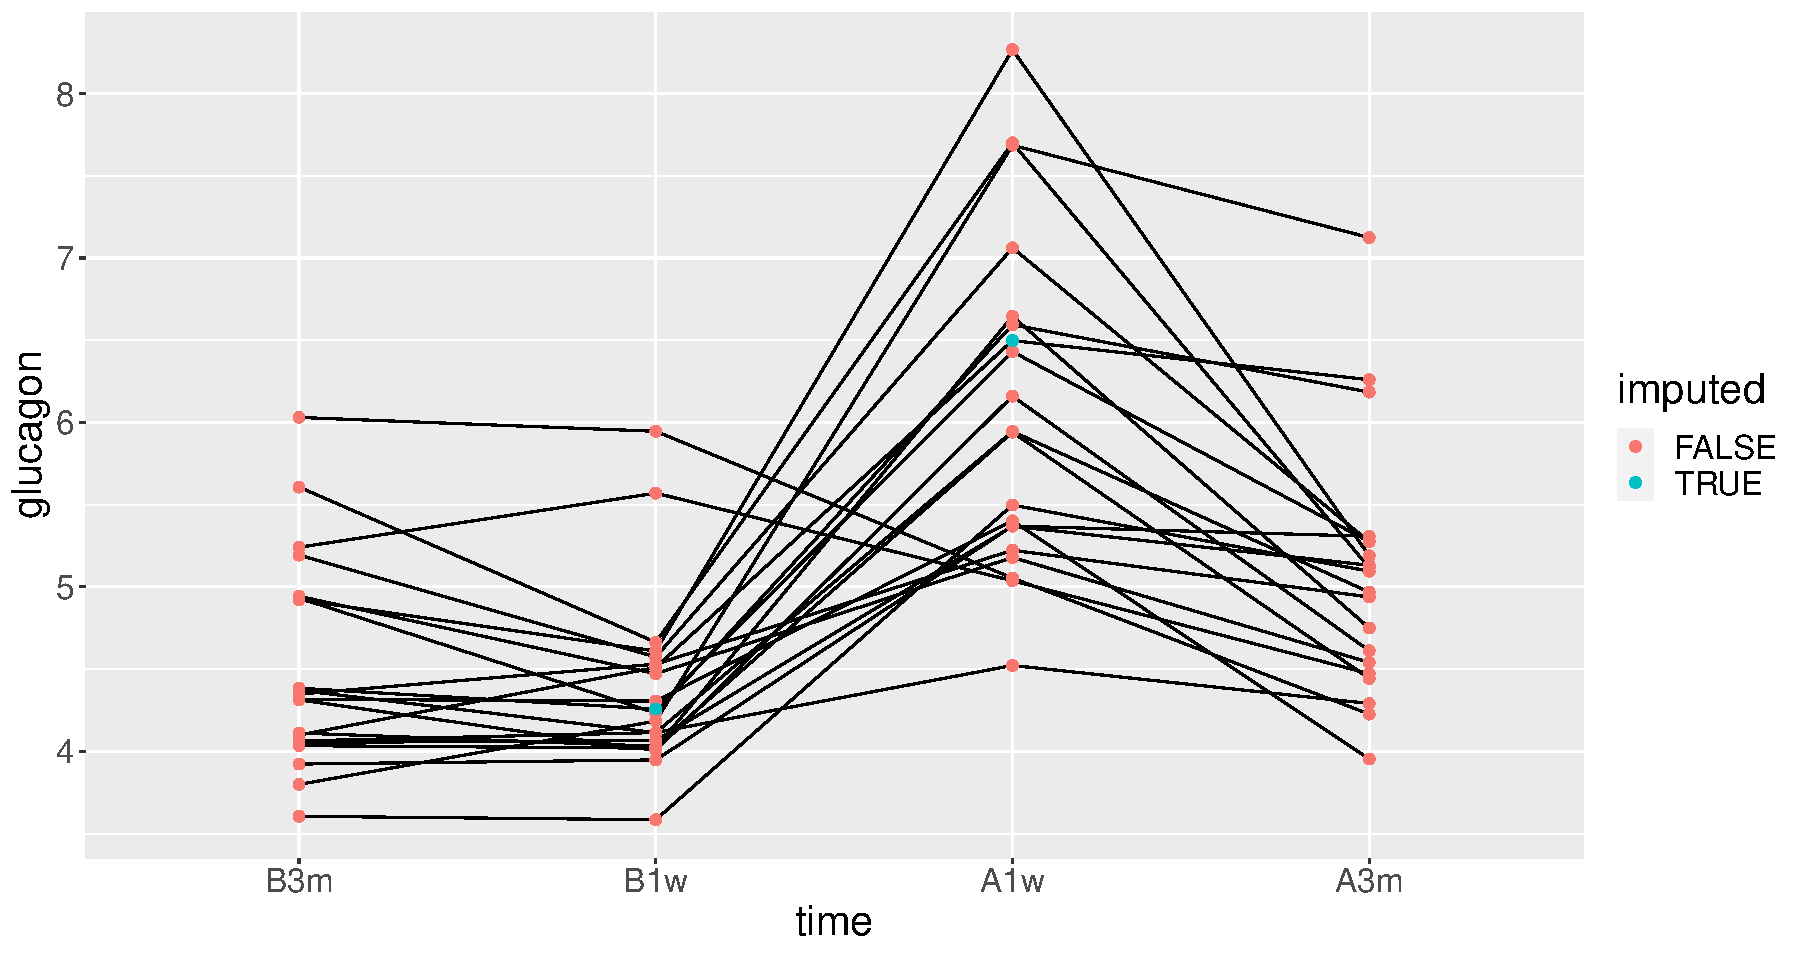
\includegraphics[trim={0 0 0 0},width=1\textwidth]{./figures/imputation.pdf}
\end{center}

It is possible to sample from the estimated distribution of the
missing value instead of using the most likely value, e.g. accounting
for residual variance and uncertainty related to parameter estimation:
\lstset{language=r,label= ,caption= ,captionpos=b,numbers=none}
\begin{lstlisting}
set.seed(10)
index.na <- which(is.na(gastricbypassL$glucagonAUC))
fitted(eUN.lmmNA, impute = TRUE, se.impute = "total")[index.na]
fitted(eUN.lmmNA, impute = TRUE, se.impute = "total")[index.na]
fitted(eUN.lmmNA, impute = TRUE, se.impute = "total")[index.na]
\end{lstlisting}

\begin{verbatim}
[1] 4.262434 6.305287
[1] 3.858267 5.871642
[1] 4.342624 6.905246
\end{verbatim}


\clearpage

\subsection{Multiple imputation}
\label{sec:org3afa1b0}

The \texttt{mlmm} function can used to perform stratify analyses, typically
useful when performing multiple imputations. Consider the wide format
of the dataset where a few values are missing:
\lstset{language=r,label= ,caption= ,captionpos=b,numbers=none}
\begin{lstlisting}
data(gastricbypassW, package = "LMMstar")
colSums(is.na(gastricbypassW))
\end{lstlisting}

\begin{verbatim}
          id      weight1      weight2      weight3      weight4 glucagonAUC1 glucagonAUC2 
           0            0            0            0            0            0            1 
glucagonAUC3 glucagonAUC4 
           1            0
\end{verbatim}


We use \texttt{mice} to generate a number of imputed datasets (here 5):
\lstset{language=r,label= ,caption= ,captionpos=b,numbers=none}
\begin{lstlisting}
library(mice)
set.seed(10)
gastricbypassW.mice <- mice(gastricbypassW, m = 5, printFlag = FALSE)
gastricbypassW.NNA <- complete(gastricbypassW.mice, action = "long")
table(gastricbypassW.NNA$.imp)
\end{lstlisting}

\begin{verbatim}
Advarselsbesked:
Number of logged events: 110

 1  2  3  4  5 
20 20 20 20 20
\end{verbatim}


We can then use \texttt{mlmm} to perform a separate linear regression per dataset:
\lstset{language=r,label= ,caption= ,captionpos=b,numbers=none}
\begin{lstlisting}
e.mlmm <- mlmm(glucagonAUC3~glucagonAUC2+weight2, data=gastricbypassW.NNA,
               by = ".imp", effects = "weight2=0", trace = FALSE)
model.tables(e.mlmm)
\end{lstlisting}

\begin{verbatim}
  by parameter  estimate       se      df     lower     upper     p.value
1  1   weight2 -204.6291 62.88617 17.0034 -337.3053 -71.95289 0.004670840
2  2   weight2 -194.4004 62.31006 17.0034 -325.8611 -62.93968 0.006231893
3  3   weight2 -211.9042 65.51654 17.0034 -350.1299 -73.67848 0.004872354
4  4   weight2 -199.8417 62.12071 17.0034 -330.9029 -68.78041 0.005058119
5  5   weight2 -199.9269 62.16057 17.0034 -331.0722 -68.78152 0.005065662
\end{verbatim}


and pool the results using Rubin's rule:
\lstset{language=r,label= ,caption= ,captionpos=b,numbers=none}
\begin{lstlisting}
model.tables(e.mlmm, method = "pool.rubin")
\end{lstlisting}

\begin{verbatim}
        estimate      se       df     lower     upper     p.value
<1, 5> -202.1404 63.4192 15.09811 -337.2388 -67.04208 0.006078676
\end{verbatim}


This matches\footnote{almost exactly, only the degrees of freedom are a
little different} the results obtained with the mice package:
\lstset{language=r,label= ,caption= ,captionpos=b,numbers=none}
\begin{lstlisting}
e.mice <- with(data=gastricbypassW.mice,exp=lm(glucagonAUC3~glucagonAUC2+weight2))
summary(pool(e.mice))
\end{lstlisting}

\begin{verbatim}
          term      estimate    std.error  statistic       df      p.value
1  (Intercept)  4.119699e+04 7674.2675772  5.3681988 15.08457 7.675819e-05
2 glucagonAUC2  7.038742e-02    0.3689445  0.1907805 15.23549 8.512165e-01
3      weight2 -2.021404e+02   63.4191998 -3.1873698 15.09481 6.080058e-03
\end{verbatim}


\clearpage

One can use the \texttt{plot} function to obtain a forest plot of the
individual estimates along with the pooled estimate:
\lstset{language=r,label= ,caption= ,captionpos=b,numbers=none}
\begin{lstlisting}
plot(e.mlmm, method = c("pool.rubin","none"))
\end{lstlisting}

\begin{center}
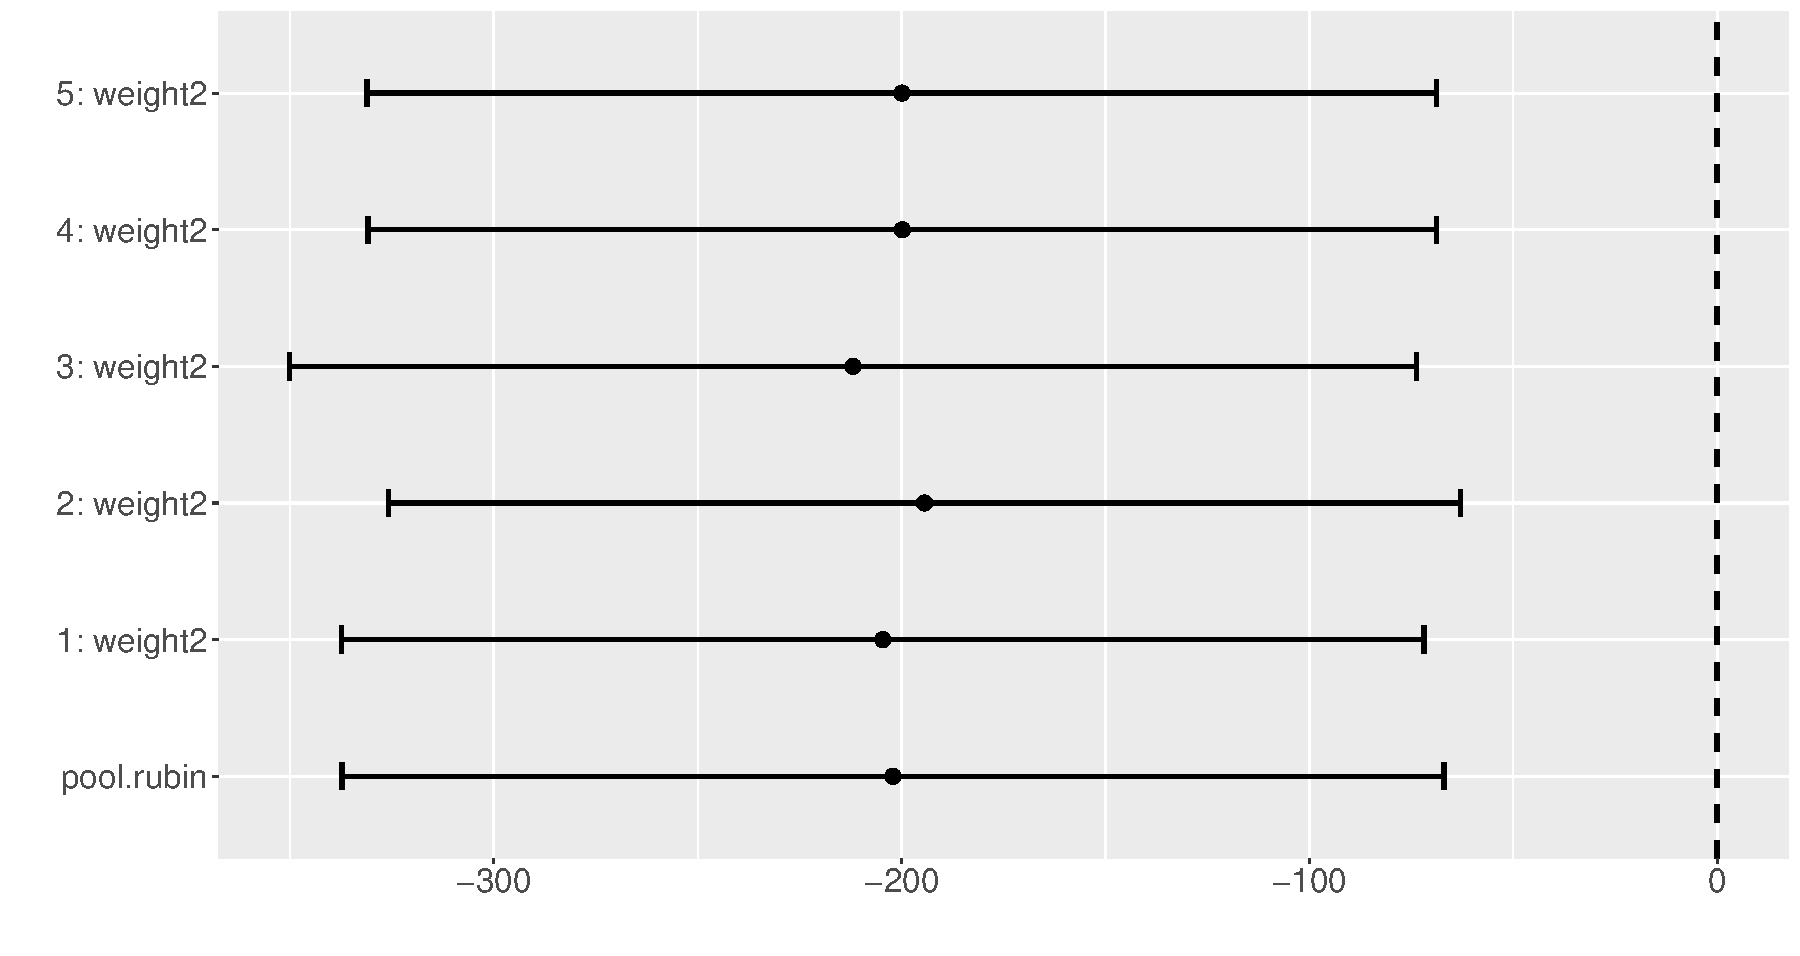
\includegraphics[trim={0 0 0 0},width=1\textwidth]{./figures/forestplot.pdf}
\end{center}

\clearpage

\section{Data generation}
\label{sec:orge9862de}
Simulate some data in the wide format:
\lstset{language=r,label= ,caption= ,captionpos=b,numbers=none}
\begin{lstlisting}
set.seed(10) ## ensure reproductibility
n.obs <- 100
n.times <- 4
mu <- rep(0,4)
gamma <- matrix(0, nrow = n.times, ncol = 10) ## add interaction
gamma[,6] <- c(0,1,1.5,1.5)
dW <- sampleRem(n.obs, n.times = n.times, mu = mu, gamma = gamma, format = "wide")
head(round(dW,3))
\end{lstlisting}

\begin{verbatim}
  id X1 X2 X3 X4 X5     X6     X7     X8    X9    X10     Y1     Y2     Y3     Y4
1  1  1  0  1  1  0 -0.367  1.534 -1.894 1.729  0.959  1.791  2.429  3.958  2.991
2  2  1  0  1  2  0 -0.410  2.065  1.766 0.761 -0.563  2.500  4.272  3.002  2.019
3  3  0  0  2  1  0 -1.720 -0.178  2.357 1.966  1.215 -3.208 -5.908 -4.277 -5.154
4  4  0  0  0  1  0  0.923 -2.089  0.233 1.307 -0.906 -2.062  0.397  1.757 -1.380
5  5  0  0  2  1  0  0.987  5.880  0.385 0.028  0.820  7.963  7.870  7.388  8.609
6  6  0  0  1  1  2 -1.075  0.479  2.202 0.900 -0.739  0.109 -1.602 -1.496 -1.841
\end{verbatim}


Simulate some data in the long format:
\lstset{language=r,label= ,caption= ,captionpos=b,numbers=none}
\begin{lstlisting}
set.seed(10) ## ensure reproductibility
dL <- sampleRem(n.obs, n.times = n.times, mu = mu, gamma = gamma, format = "long")
head(dL)
\end{lstlisting}

\begin{verbatim}
  id visit        Y X1 X2 X3 X4 X5         X6       X7        X8        X9        X10
1  1     1 1.791444  1  0  1  1  0 -0.3665251 1.533815 -1.894425 1.7288665  0.9592499
2  1     2 2.428570  1  0  1  1  0 -0.3665251 1.533815 -1.894425 1.7288665  0.9592499
3  1     3 3.958350  1  0  1  1  0 -0.3665251 1.533815 -1.894425 1.7288665  0.9592499
4  1     4 2.991198  1  0  1  1  0 -0.3665251 1.533815 -1.894425 1.7288665  0.9592499
5  2     1 2.500179  1  0  1  2  0 -0.4097541 2.065413  1.765841 0.7613348 -0.5630173
6  2     2 4.272357  1  0  1  2  0 -0.4097541 2.065413  1.765841 0.7613348 -0.5630173
\end{verbatim}


\clearpage

\section{Modifying default options}
\label{sec:org7cd1f66}
The \texttt{LMMstar.options} method enable to get and set the default options
used by the package. For instance, the default option for the information matrix is:
\lstset{language=r,label= ,caption= ,captionpos=b,numbers=none}
\begin{lstlisting}
LMMstar.options("type.information")
\end{lstlisting}

\begin{verbatim}
$type.information
[1] "observed"
\end{verbatim}


To change the default option to "expected" (faster to compute but less accurate p-values and confidence intervals in small samples) use:
\lstset{language=r,label= ,caption= ,captionpos=b,numbers=none}
\begin{lstlisting}
LMMstar.options(type.information = "expected")
\end{lstlisting}

To restore the original default options do:
\lstset{language=r,label= ,caption= ,captionpos=b,numbers=none}
\begin{lstlisting}
LMMstar.options(reinitialise = TRUE)
\end{lstlisting}

\clearpage

\section{R session}
\label{sec:org76ebe9e}
Details of the R session used to generate this document:
\lstset{language=r,label= ,caption= ,captionpos=b,numbers=none}
\begin{lstlisting}
sessionInfo()
\end{lstlisting}

\begin{verbatim}
R version 4.2.0 (2022-04-22 ucrt)
Platform: x86_64-w64-mingw32/x64 (64-bit)
Running under: Windows 10 x64 (build 19045)

Matrix products: default

locale:
[1] LC_COLLATE=Danish_Denmark.utf8  LC_CTYPE=Danish_Denmark.utf8    LC_MONETARY=Danish_Denmark.utf8
[4] LC_NUMERIC=C                    LC_TIME=Danish_Denmark.utf8    

attached base packages:
[1] parallel  grid      stats     graphics  grDevices utils     datasets  methods   base     

other attached packages:
 [1] mice_3.14.0          sandwich_3.0-2       scales_1.2.1         rlang_1.1.1         
 [5] pbapply_1.7-0        numDeriv_2016.8-1.1  nlme_3.1-158         lava_1.7.2.1        
 [9] doSNOW_1.0.20        snow_0.4-4           iterators_1.0.14     foreach_1.5.2       
[13] copula_1.1-2         lme4_1.1-29          Matrix_1.5-1         LMMstar_1.0.0       
[17] ggpubr_0.4.0         multcomp_1.4-22      TH.data_1.1-1        MASS_7.3-57         
[21] survival_3.3-1       mvtnorm_1.2-3        qqtest_1.2.0         emmeans_1.8.8-090002
[25] ggplot2_3.4.3       

loaded via a namespace (and not attached):
 [1] butils.base_1.2     minqa_1.2.4         colorspace_2.1-0    ggsignif_0.6.3     
 [5] ellipsis_0.3.2      estimability_1.4.1  parameters_0.18.2   fs_1.6.3           
 [9] listenv_0.9.0       farver_2.1.1        remotes_2.4.2       gsl_2.1-8          
[13] fansi_1.0.4         codetools_0.2-18    splines_4.2.0       doParallel_1.0.17  
[17] cachem_1.0.8        pkgload_1.3.0       nloptr_2.0.3        broom_0.8.0        
[21] stabledist_0.7-1    effectsize_0.7.0.5  shiny_1.7.2         compiler_4.2.0     
[25] backports_1.4.1     fastmap_1.1.1       cli_3.6.1           later_1.3.0        
[29] htmltools_0.5.6     prettyunits_1.1.1   tools_4.2.0         lmerTest_3.1-3     
[33] coda_0.19-4         gtable_0.3.4        glue_1.6.2          reshape2_1.4.4     
[37] dplyr_1.1.3         Rcpp_1.0.11         carData_3.0-5       vctrs_0.6.3        
[41] insight_0.18.4      stringr_1.5.0       globals_0.16.2      ps_1.7.1           
[45] mime_0.12           miniUI_0.1.1.1      lifecycle_1.0.3     devtools_2.4.4     
[49] rstatix_0.7.0       future_1.31.0       zoo_1.8-11          promises_1.2.0.1   
[53] memoise_2.0.1       gridExtra_2.3       stringi_1.7.12      bayestestR_0.13.0  
[57] pcaPP_2.0-3         boot_1.3-28         pkgbuild_1.3.1      pkgconfig_2.0.3    
[61] lattice_0.20-45     purrr_1.0.2         htmlwidgets_1.6.2   labeling_0.4.3     
[65] cowplot_1.1.1       tidyselect_1.2.0    processx_3.6.1      parallelly_1.34.0  
[69] plyr_1.8.7          magrittr_2.0.3      R6_2.5.1            generics_0.1.3     
[73] profvis_0.3.7       ADGofTest_0.3       pillar_1.9.0        withr_2.5.1        
[77] mgcv_1.8-40         datawizard_0.6.1    abind_1.4-5         pspline_1.0-19     
[81] tibble_3.2.1        future.apply_1.10.0 crayon_1.5.1        car_3.1-0          
[85] utf8_1.2.3          urlchecker_1.0.1    usethis_2.1.6       data.table_1.14.2  
[89] callr_3.7.2         digest_0.6.33       xtable_1.8-4        tidyr_1.3.0        
[93] httpuv_1.6.5        stats4_4.2.0        munsell_0.5.0       sessioninfo_1.2.2
\end{verbatim}

\clearpage

\section*{References}
\label{sec:org704fd46}
\begingroup
\renewcommand{\section}[2]{}

\bibliographystyle{apalike}
\bibliography{bibliography}

\endgroup

\clearpage

\appendix
\titleformat{\section}
{\normalfont\Large\bfseries}{Appendix~\thesection}{1em}{}

\renewcommand{\thefigure}{\Alph{figure}}
\renewcommand{\thetable}{\Alph{table}}
\renewcommand{\theequation}{\Alph{equation}}

\setcounter{figure}{0}    
\setcounter{table}{0}    
\setcounter{equation}{0}    

\section{Likelihood in a linear mixed model}
\label{SM:likelihood}
Denote by \(\VY\) a vector of \(m\) outcomes, \(\VX\) a vector of
\(p\) covariates, \(\mu(\Vparam,\VX)\) the modeled mean, and
\(\Omega(\Vparam,\VX)\) the modeled residual variance-covariance. We
consider \(n\) replicates (i.e. \(\VY_1,\ldots,\VY_n)\) and
\(VX_1,\ldots,\VX_n\)) along with a vector of weights
\(\omega=(w_1,\ldots,w_n)\), which are by default all equal to 1.

\subsection{Log-likelihood}
\label{sec:orgb510d84}

The restricted log-likelihood in a linear mixed model can then be
written:
\begin{align}
\Likelihood(\Vparam|\VY,\VX) =& \textcolor{\darkred}{ \frac{p}{2} \log(2\pi)-\frac{1}{2} \log\left(\left|\sum_{i=1}^n w_i \VX_i \Omega_i^{-1}(\Vparam) \trans{\VX}_i\right|\right)} \notag \\
& + \sum_{i=1}^{n} w_i \left(\textcolor{\darkblue}{-\frac{m}{2} \log(2\pi) - \frac{1}{2} \log\left|\Omega_i(\Vparam)\right| - \frac{1}{2} (\VY_i-\mu(\Vparam,\VX_i)) \Omega_i(\Vparam)^{-1} \trans{(\VY_i-\mu(\Vparam,\VX_i))}} \right)  \label{eq:log-likelihood}
\end{align}

This is what the \texttt{logLik} method is computing for the REML
criteria. The red term is specific to the REML criteria and prevents
from computing individual contributions to the likelihood\footnote{The REML is the
likelihood of the observations divided by the prior on the estimated
mean parameters \(\VparamHat_{\mu} \sim \Gaus(\mu,\left(\VX
 \Omega^{-1}(\Vparam) \trans{\VX}\right)^{-1})\). This corresponds to
\(\frac{1}{\sqrt{2\pi}^p \left|\left(\sum_{i=1}^n \VX_i
 \Omega_i^{-1}(\Vparam) \trans{\VX}_i\right)^{-1}\right|}
 \exp\left(-(\VparamHat_{\mu}-\mu)\left(2\sum_{i=1}^n \VX_i
 \Omega_i^{-1}(\Vparam)
 \trans{\VX}_i\right)^{-1})\trans{(\VparamHat_{\mu}-\mu)}\right)\)
Since \(\mu\) will be estimated to be \(\Vparam_{\mu}\), the
exponential term equals 1 and thus does not contribute to the
log-likelihood. One divided by the other term gives \(\sqrt{2\pi}^p
 \left(\left|\sum_{i=1}^n \VX_i \Omega_i^{-1}(\Vparam)
 \trans{\VX}_i\right|\right)^{-1}\). The log of this term equals the red
term}. The blue term is what \texttt{logLik} outputs for the ML criteria
when setting the argument \texttt{indiv} to \texttt{TRUE}.

\bigskip

\subsection{Score}
\label{sec:org5c52188}

 Using that \(\partial \log(\det(X))=tr(X^{-1}\partial(X))\), the
score is obtained by derivating once the log-likelihood, i.e., for
\(\theta \in \Vparam\):
\begin{align*}
   \Score(\theta) =& \dpartial[\Likelihood(\Vparam|\VY,\VX)][\theta]
= \textcolor{\darkred}{ \frac{1}{2} tr \left( \left(\sum_{i=1}^n w_i \VX_i \Omega_i^{-1}(\Vparam) \trans{\VX}_i\right)^{-1} \left(\sum_{i=1}^n w_i \VX_i \Omega_i^{-1}(\Vparam) \dpartial[\Omega_i(\Vparam)][\theta] \Omega_i(\Vparam)^{-1} \trans{\VX}_i\right)  \right) } \\
&+ \sum_{i=1}^n w_i \left( \textcolor{\darkblue}{ -\frac{1}{2} tr\left(\Omega_i(\Vparam)^{-1} \dpartial[\Omega_i(\Vparam)][\theta]\right) + \dpartial[\mu(\Vparam,\VX_i)][\theta] \Omega_i(\Vparam)^{-1} \trans{(\VY_i-\mu(\Vparam,\VX_i))} } \right. \\
 & \qquad \qquad \left. \textcolor{\darkblue}{ + \frac{1}{2} (\VY_i-\mu(\Vparam,\VX_i)) \Omega_i(\Vparam)^{-1} \dpartial[\Omega_i(\Vparam)][\theta] \Omega_i(\Vparam)^{-1} \trans{(\VY_i-\mu(\Vparam,\VX_i))} } \right).
\end{align*}

This is what the \texttt{score} method is computing for the REML
criteria. The red term is specific to the REML criteria and prevents
from computing the score relative to each cluster. The blue term is
what \texttt{score} outputs for the ML criteria when setting the argument
\texttt{indiv} to \texttt{TRUE}.

\bigskip

\clearpage

\subsection{Hessian}
\label{sec:org0cfe978}

Derivating a second time the log-likelihood gives the hessian, \(\Hessian(\Vparam)\), with element\footnote{if one is relative to the mean and the other to the variance then they are respectively \(\theta\) and \(\theta'\)}:
\begin{align*}
& \Hessian(\theta,\theta^{\prime}) = \ddpartial[\Likelihood(\Vparam|\VY,\VX)][\theta][\theta^{\prime}] = \dpartial[\Score(\theta)][\theta^{\prime}] \\
=& \textcolor{\darkred}{\frac{1}{2} tr \left( \left(\sum_{i=1}^n w_i \VX_i \Omega_i^{-1}(\Vparam) \trans{\VX}_i\right)^{-1} \left\{ \sum_{i=1}^n w_i \VX_i \Omega_i^{-1}(\Vparam) \left(\ddpartial[\Omega_i(\Vparam)][\theta][\theta^{\prime}] - 2 \dpartial[\Omega_i(\Vparam)][\theta] \Omega_i^{-1}(\Vparam) \dpartial[\Omega_i(\Vparam)][\theta^{\prime}]\right)\Omega_i(\Vparam)^{-1} \trans{\VX}_i \right.  \right.}  \\
& \textcolor{\darkred}{ \left. \left. + \left(\sum_{i=1}^n w_i \VX_i \Omega_i^{-1}(\Vparam) \dpartial[\Omega_i(\Vparam)][\theta] \Omega_i(\Vparam)^{-1} \trans{\VX}_i\right) \left(\sum_{i=1}^n w_i \VX_i\Omega_i^{-1}(\Vparam) \trans{\VX}_i \right)^{-1} \left(\sum_{i=1}^n w_i \VX_i \Omega_i^{-1}(\Vparam) \dpartial[\Omega_i(\Vparam)][\theta^{\prime}] \Omega_i(\Vparam)^{-1} \trans{\VX}_i\right) \right\} \right) } \\
& +\sum_{i=1}^n w_i \left( \textcolor{\darkblue}{ \frac{1}{2} tr\left(\Omega_i(\Vparam)^{-1} \dpartial[\Omega_i(\Vparam)][\theta^{\prime}] \Omega_i(\Vparam)^{-1} \dpartial[\Omega_i(\Vparam)][\theta] - \Omega_i(\Vparam)^{-1} \ddpartial[\Omega_i(\Vparam)][\theta][\theta^{\prime}] \right) } \right.\\
& \qquad \textcolor{\darkblue}{ -  \dpartial[\mu(\Vparam,\VX_i)][\theta] \Omega_i(\Vparam)^{-1} \dpartial[\Omega_i(\Vparam)][\theta^{\prime}] \Omega_i(\Vparam)^{-1} \trans{\Vvarepsilon_i(\Vparam)} - \dpartial[\mu(\Vparam,\VX_i)][\theta] \Omega_i(\Vparam)^{-1} \trans{\dpartial[\mu(\Vparam,\VX_i)][\theta^{\prime}]} } \\
& \qquad \left. \textcolor{\darkblue}{ + \frac{1}{2} \Vvarepsilon_i(\Vparam) \Omega_i(\Vparam)^{-1} \left(\ddpartial[\Omega_i(\Vparam)][\theta][\theta^{\prime}] - \dpartial[\Omega_i(\Vparam)][\theta^{\prime}] \Omega_i(\Vparam)^{-1} \dpartial[\Omega_i(\Vparam)][\theta] - \dpartial[\Omega_i(\Vparam)][\theta] \Omega_i(\Vparam)^{-1} \dpartial[\Omega_i(\Vparam)][\theta^{\prime}] \right) \Omega_i(\Vparam)^{-1} \trans{\Vvarepsilon_i(\Vparam)} } \right).
\end{align*}
where \(\Vvarepsilon_i(\Vparam) = \VY_i-\mu(\Vparam,\VX_i)\).

\bigskip

The \texttt{information} method will (by default) return the (observed)
information which is the opposite of the hessian. So multiplying the
previous formula by -1 gives what \texttt{information} output for the REML
criteria. The red term is specific to the REML criteria and prevents
from computing the information relative to each cluster. The blue term
is what \texttt{information} outputs for the ML criteria (up to a factor -1)
when setting the argument \texttt{indiv} to \texttt{TRUE}.

\bigskip

A possible simplification is to use the expected hessian at the maximum likelihood. Indeed for
any deterministic matrix \(A\):
\begin{itemize}
\item \(\Esp[A \trans{(\VY_i-\mu(\Vparam,\VX_i))}|\VX_i] = 0\)
\item \(\Esp[(\VY_i-\mu(\Vparam,\VX_i)) A \trans{(\VY_i-\mu(\Vparam,\VX_i))}||\VX_i] = tr(A \Var(\VY_i-\mu(\Vparam,\VX_i)))\)
\end{itemize}
when \(\Esp[\VY_i-\mu(\Vparam,\VX_i)]=0\). This leads to:
\begin{align}
 & \Esp[\Hessian(\theta,\theta^{\prime})|\VX] \notag\\ 
 &= \textcolor{\darkred}{ \frac{1}{2} tr \left( \left(\sum_{i=1}^n w_i \VX_i \Omega_i^{-1}(\Vparam) \trans{\VX}_i\right)^{-1}  \left\{ \sum_{i=1}^n w_i \VX_i \Omega_i^{-1}(\Vparam) \left( \ddpartial[\Omega_i(\Vparam)][\theta][\theta^{\prime}] - 2 \dpartial[\Omega_i(\Vparam)][\theta]  \Omega_i^{-1}(\Vparam) \dpartial[\Omega_i(\Vparam)][\theta^{\prime}]\right) \Omega_i(\Vparam)^{-1} \trans{\VX}_i \right.  \right.} \notag \\
 & \textcolor{\darkred}{ \left. \left. +  \left(\sum_{i=1}^n w_i \VX_i \Omega_i^{-1}(\Vparam) \dpartial[\Omega_i(\Vparam)][\theta] \Omega_i(\Vparam)^{-1} \trans{\VX}_i\right) \left(\sum_{i=1}^n w_i \VX_i \Omega_i^{-1}(\Vparam) \trans{\VX}_i \right)^{-1} \left(\sum_{i=1}^n w_i \VX_i \Omega_i^{-1}(\Vparam) \dpartial[\Omega_i(\Vparam)][\theta^{\prime}] \Omega_i(\Vparam)^{-1} \trans{\VX}_i\right) \right\} \right) } \notag\\
 & + \sum_{i=1}^n w_i \left( \textcolor{\darkblue}{
- \frac{1}{2} tr\left(\Omega_i(\Vparam)^{-1} \dpartial[\Omega_i(\Vparam)][\theta^{\prime}] \Omega_i(\Vparam)^{-1} \dpartial[\Omega_i(\Vparam)][\theta]\right)
 - \dpartial[\mu(\Vparam,\VX_i)][\theta] \Omega_i(\Vparam)^{-1} \trans{\dpartial[\mu(\Vparam,\VX_i)][\theta^{\prime}]}
 } \right) \label{eq:expectedInfo}
\end{align}

This is what \texttt{information} output when the argument \texttt{type.information}
is set to \texttt{"expected"} (up to a factor -1).

\clearpage

\subsection{Degrees of freedom}
\label{sec:org5ea9e75}

Degrees of freedom are computed using a Satterthwaite approximation,
i.e. for an estimate coefficient \(\widehat{\beta}\in\widehat{\Vparam}\) with standard
error \(\sigma_{\widehat{\beta}}\), the degree of freedom is:
\begin{align*}
df\left(\sigma_{\widehat{\beta}}\right) = \frac{2 \sigma^4_{\widehat{\beta}}}{\Var[\widehat{\sigma}_{\widehat{\beta}}]}
\end{align*}
Using a first order Taylor expansion we can approximate the variance term as:
\begin{align*}
\Var[\widehat{\sigma}_{\widehat{\beta}}] & \approx \dpartial[\widehat{\sigma}_{\widehat{\beta}}][\Vparam] \Sigma_{\Vparam}  \trans{\dpartial[\widehat{\sigma}_{\widehat{\beta}}][\Vparam]} \\
& \approx c_{\beta} \left(\widehat{\Information}_{\widehat{\Vparam}}\right)^{-1} \dpartial[\widehat{\Information}_{\widehat{\Vparam}}][\Vparam] \left(\widehat{\Information}_{\widehat{\Vparam}}\right)^{-1} \trans{c_{\beta}} \Sigma_{\Vparam} \trans{c_{\beta}} \left(\widehat{\Information}_{\widehat{\Vparam}}\right)^{-1} \trans{\dpartial[\widehat{\Information}_{\widehat{\Vparam}}][\Vparam]} \left(\widehat{\Information}_{\widehat{\Vparam}}\right)^{-1} c_{\beta}
\end{align*}

where \(\Sigma_{\Vparam}\) is the variance-covariance matrix of all
  model coefficients, \(\Information_{\Vparam}\) the information
  matrix for all model coefficients, \(c_{\beta}\) a matrix used to
  select the element relative to \(\beta\) in the first derivative of
  the information matrix, and \(\dpartial[.][\Vparam]\) denotes the
  vector of derivatives with respect to all model coefficients.

\bigskip

The derivative of the information matrix (i.e. negative hessian) can
then be computed using numerical derivatives or using analytical
formula. To obtain the later we first notice that:
\begin{align}
&\Hessian(\theta,\theta^{\prime}) = \Esp[\Hessian(\theta,\theta^{\prime})|\VX] \notag \\
& + \sum_{i=1}^n  w_i \left( \textcolor{\darkblue}{ tr\left(\Omega_i(\Vparam)^{-1} \dpartial[\Omega_i(\Vparam)][\theta^{\prime}] \Omega_i(\Vparam)^{-1} \dpartial[\Omega_i(\Vparam)][\theta] - \Omega_i(\Vparam)^{-1} \ddpartial[\Omega_i(\Vparam)][\theta][\theta^{\prime}] \right) } \right. \notag \\
& \qquad \textcolor{\darkblue}{ -  \dpartial[\mu(\Vparam,\VX_i)][\theta] \Omega_i(\Vparam)^{-1} \dpartial[\Omega_i(\Vparam)][\theta^{\prime}] \Omega_i(\Vparam)^{-1} \trans{\Vvarepsilon_i(\Vparam)}} \notag \\
& \qquad \left. \textcolor{\darkblue}{ + \frac{1}{2} \Vvarepsilon_i(\Vparam) \Omega_i(\Vparam)^{-1} \left(\ddpartial[\Omega_i(\Vparam)][\theta][\theta^{\prime}] - \dpartial[\Omega_i(\Vparam)][\theta^{\prime}] \Omega_i(\Vparam)^{-1} \dpartial[\Omega_i(\Vparam)][\theta] - \dpartial[\Omega_i(\Vparam)][\theta] \Omega_i(\Vparam)^{-1} \dpartial[\Omega_i(\Vparam)][\theta^{\prime}] \right) \Omega_i(\Vparam)^{-1} \trans{\Vvarepsilon_i(\Vparam)} } \right) \label{eq:diffInfo}
\end{align}
where
\begin{align*}
\Esp[\Hessian(\theta,\theta^{\prime})|\VX] &=& \textcolor{\darkred}{
\frac{1}{2} tr \left(A(\Vparam)^{-1} \left(\sum_{i=1}^n w_i b_i(\Vparam) B_i(\Vparam) \trans{b}_i(\Vparam) + C(\Vparam)A(\Vparam)^{-1} \trans{C}(\Vparam) \right)\right)
}  + \sum_{i=1}^n w_i \textcolor{\darkblue}{E_i(\Vparam)} \\
\textcolor{\darkblue}{E_i(\Vparam)} &=& \textcolor{\darkblue}{\frac{1}{2} tr\left(\Omega_i(\Vparam)^{-1} \dpartial[\Omega_i(\Vparam)][\theta^{\prime}] \Omega_i(\Vparam)^{-1} \dpartial[\Omega_i(\Vparam)][\theta]\right)
                                        - \dpartial[\mu(\Vparam,\VX_i)][\theta] \Omega_i(\Vparam)^{-1} \trans{\dpartial[\mu(\Vparam,\VX_i)][\theta^{\prime}]}} \\
\textcolor{\darkred}{A(\Theta)} &=& \textcolor{\darkred}{\sum_{i=1}^n w_i \VX_i \Omega_i^{-1}(\Vparam) \trans{\VX}_i }\\
\textcolor{\darkred}{B(\Theta)} &=& \textcolor{\darkred}{\ddpartial[\Omega_i(\Vparam)][\theta][\theta^{\prime}] - 2 \dpartial[\Omega_i(\Vparam)][\theta]  \Omega_i^{-1}(\Vparam) \dpartial[\Omega_i(\Vparam)][\theta^{\prime}] }\\
\textcolor{\darkred}{b_i(\Theta)} &=& \textcolor{\darkred}{\VX_i \Omega_i^{-1} }\\
\textcolor{\darkred}{C(\Theta)} &=& \textcolor{\darkred}{\sum_{i=1}^n w_i \VX_i \Omega_i^{-1}(\Vparam) \dpartial[\Omega_i(\Vparam)][\theta] \Omega_i(\Vparam)^{-1} \trans{\VX}_i }
\end{align*}
So we will first derive the derivative of
\(\Esp[\Hessian(\theta,\theta^{\prime})|\VX]\) and then the one of the
blue term in \autoref{eq:diffInfo}.  To simplify the derivation of the
formula we will only derive them at the maximum likelihood, i.e. when
\(\Esp\left[\dpartial[\Hessian(\theta,\theta^{\prime}|\VX)][\theta^{\prime\prime}]\right]=\frac{\partial
\Esp[\Hessian(\theta,\theta^{\prime}|\VX)]}{\partial
\theta^{\prime\prime}}\) where the expectation is taken over
\(\VX\). We first notice that the derivative with respect to the mean
parameters is 0. So we just need to compute the derivative with
respect to a variance parameter \(\theta^{\prime\prime}\):
\begin{align*}
 & \frac{\partial \textcolor{\darkred}{ A(\Vparam)^{-1} \left(\sum_{i=1}^n w_i b_i(\Vparam) B_i(\Vparam) \trans{b}_i(\Vparam) + C(\Vparam)A(\Vparam)^{-1} \trans{C}(\Vparam) \right)}}{\partial \theta^{\prime\prime}} \\
 =& \textcolor{\darkred}{A(\Vparam)^{-1} \dpartial[A(\Vparam)][\theta^{\prime\prime}] A(\Vparam)^{-1} \left(\sum_{i=1}^n w_i b_i(\Vparam) B_i(\Vparam) \trans{b}_i(\Vparam) + C(\Vparam)A(\Vparam)^{-1} \trans{C}(\Vparam) \right)} \\
 & +\textcolor{\darkred}{A(\Vparam)^{-1} \left(\sum_{i=1}^n w_i \left(
 \dpartial[b_i(\Vparam)][\theta^{\prime\prime}]  B_i(\Vparam) \trans{b}_i(\Vparam)
 + b_i(\Vparam) \dpartial[B_i(\Vparam)][\theta^{\prime\prime}]   \trans{b}_i(\Vparam)
 + b_i(\Vparam) B_i(\Vparam) \dpartial[\trans{b}_i(\Vparam)][\theta^{\prime\prime}] \right. \right. } \\
& \qquad \qquad \qquad \qquad \quad + \textcolor{\darkred}{\left. \left.
 \dpartial[C(\Vparam)][\theta^{\prime\prime}]  A^{-1}(\Vparam) \trans{C}(\Vparam)
 + C(\Vparam) A^{-1}\dpartial[A(\Vparam)][\theta^{\prime\prime}]A^{-1}   \trans{C}(\Vparam)
 + C(\Vparam) A^{-1}(\Vparam) \dpartial[\trans{C}(\Vparam)][\theta^{\prime\prime}]
\right) \right)}
\end{align*}

and

\begin{align*}
 \dpartial[\textcolor{\darkblue}{E(\Vparam)}][\theta^{\prime\prime}]=&
 \sum_{i=1}^n w_i \left( \textcolor{\darkblue}{
- \frac{1}{2} tr\left(
-2\Omega_i(\Vparam)^{-1} \dpartial[\Omega_i(\Vparam)][\theta^{\prime\prime}] \Omega_i(\Vparam)^{-1} \dpartial[\Omega_i(\Vparam)][\theta^{\prime}] \Omega_i(\Vparam)^{-1} \dpartial[\Omega_i(\Vparam)][\theta] \right. } \right. \\
& \qquad \qquad \textcolor{\darkblue}{\left. + \Omega_i(\Vparam)^{-1} \ddpartial[\Omega_i(\Vparam)][\theta^{\prime}][\theta^{\prime\prime}] \Omega_i(\Vparam)^{-1} \dpartial[\Omega_i(\Vparam)][\theta]
+ \Omega_i(\Vparam)^{-1} \dpartial[\Omega_i(\Vparam)][\theta^{\prime}] \Omega_i(\Vparam)^{-1} \ddpartial[\Omega_i(\Vparam)][\theta][\theta^{\prime\prime}]
\right)} \\
& \qquad \qquad  \textcolor{\darkblue}{\left. + \dpartial[\mu(\Vparam,\VX_i)][\theta] \Omega_i(\Vparam)^{-1} \dpartial[\Omega_i(\Vparam)][\theta^{\prime\prime}] \Omega_i(\Vparam)^{-1}   \trans{\dpartial[\mu(\Vparam,\VX_i)][\theta^{\prime}]}
 \right)}
\end{align*}

where:
\begin{align*}
\textcolor{\darkred}{\dpartial[A(\Vparam)][\theta^{\prime\prime}]} &= \textcolor{\darkred}{\sum_{i=1}^n w_i \VX_i \Omega^{-1}_i(\Vparam) \dpartial[\Omega_i(\Vparam)][\theta^{\prime\prime}]\Omega^{-1}_i(\Vparam) \trans{\VX}_i} \\
\textcolor{\darkred}{\dpartial[b_i(\Vparam)][\theta^{\prime\prime}]} &= \textcolor{\darkred}{\VX_i \Omega^{-1}_i(\Vparam) \dpartial[\Omega_i(\Vparam)][\theta^{\prime\prime}]\Omega^{-1}_i(\Vparam)} \\
\textcolor{\darkred}{\dpartial[B_i(\Vparam)][\theta^{\prime\prime}]} &= \textcolor{\darkred}{
  \frac{\partial^3 \Omega_i(\Vparam)}{\theta\theta^{\prime}\theta^{\prime\prime}} } \\
  & \textcolor{\darkred}{ - 2 \left(
  \ddpartial[\Omega_i(\Vparam)][\theta][\theta^{\prime\prime}]\Omega^{-1}_i(\Vparam)\dpartial[\Omega_i(\Vparam)][\theta^{\prime}]
+ \dpartial[\Omega_i(\Vparam)][\theta]\Omega^{-1}_i(\Vparam)\dpartial[\Omega_i(\Vparam)][\theta^{\prime\prime}]\Omega^{-1}_i(\Vparam)\dpartial[\Omega_i(\Vparam)][\theta^{\prime}]
+ \dpartial[\Omega_i(\Vparam)][\theta]\Omega^{-1}_i(\Vparam)\ddpartial[\Omega_i(\Vparam)][\theta^{\prime}][\theta^{\prime\prime}]
\right)
  } \\
\textcolor{\darkred}{\dpartial[C(\Vparam)][\theta^{\prime\prime}]} &= \textcolor{\darkred}{\sum_{i=1}^n w_i \VX_i \Omega^{-1}_i(\Vparam) \left(
\dpartial[\Omega_i(\Vparam)][\theta^{\prime\prime}] \Omega^{-1}_i(\Vparam) \dpartial[\Omega_i(\Vparam)][\theta]
+ \ddpartial[\Omega_i(\Vparam)][\theta][\theta^{\prime\prime}]
+ \dpartial[\Omega_i(\Vparam)][\theta] \Omega^{-1}_i(\Vparam) \dpartial[\Omega_i(\Vparam)][\theta^{\prime\prime}]
\right) \Omega^{-1}_i(\Vparam) \trans{\VX}_i} 
\end{align*}



\clearpage

\section{Likelihood ratio test with the REML criterion}
\label{SM:LRT-REML}
The blue term of \autoref{eq:log-likelihood} in the log-likelihood is
invariant to re-parameterisation while the red term is not. This means
that a re-parametrisation of \(X\) into \(\tilde{X} = B X\) with \(B\)
invertible would not change the likelihood when using ML but would
decrease the log-likelihood by \(\log(|B|)\) when using REML. \newline
Let's take an example:
\lstset{language=r,label= ,caption= ,captionpos=b,numbers=none}
\begin{lstlisting}
## data(dfL, package = "LMMstar")
dfTest <- dfL
dfTest$glucagon2 <- dfTest$glucagon*2
\end{lstlisting}

where we multiply one column of the design matrix by 2. As mentionned
previously this does not affect the log-likelihood when using ML:
\lstset{language=r,label= ,caption= ,captionpos=b,numbers=none}
\begin{lstlisting}
eML.lmmUN <- lmm(weight ~ time+glucagon, data = dfTest, repetition = ~time|id, method = "ML")
eML.lmmUN2 <- lmm(weight ~ time+glucagon2, data = dfTest, repetition = ~time|id, method = "ML")
\end{lstlisting}

\lstset{language=r,label= ,caption= ,captionpos=b,numbers=none}
\begin{lstlisting}
logLik(eML.lmmUN)
logLik(eML.lmmUN2)
\end{lstlisting}

\begin{verbatim}
[1] -218.71
[1] -218.71
\end{verbatim}


but it does when using REML:
\lstset{language=r,label= ,caption= ,captionpos=b,numbers=none}
\begin{lstlisting}
eREML.lmmUN <- lmm(weight ~ time + glucagon, data = dfTest, repetition = ~time|id, method = "REML")
eREML.lmmUN2 <- lmm(weight ~ time + glucagon2, data = dfTest, repetition = ~time|id, method = "REML")
\end{lstlisting}

\lstset{language=r,label= ,caption= ,captionpos=b,numbers=none}
\begin{lstlisting}
logLik(eREML.lmmUN)-logLik(eREML.lmmUN2)
log(2)
\end{lstlisting}

\begin{verbatim}
[1] 0.6931472
[1] 0.6931472
\end{verbatim}


Therefore, when comparing models with different mean effects there is
a risk that the difference (or part of it) in log-likelihood is due to
a new parametrisation and no only to a difference in model fit. This
would typically be the case when adding an interaction where we can
have a smaller restricted log-likehood when considering a more complex
model:

\lstset{language=r,label= ,caption= ,captionpos=b,numbers=none}
\begin{lstlisting}
set.seed(5) 
dfTest$ff <- rbinom(NROW(dfTest), size = 1, prob = 0.5)
logLik(lmm(weight ~ time+glucagon, data = dfTest, repetition = ~time|id, method = "REML"))
logLik(lmm(weight ~ time+glucagon*ff, data = dfTest, repetition = ~time|id, method = "REML"))
\end{lstlisting}

\begin{verbatim}
[1] -216.3189
[1] -216.8425
\end{verbatim}


This is quite counter-intuitive as more complex model should lead to
better fit and would never happen when using ML:
\lstset{language=r,label= ,caption= ,captionpos=b,numbers=none}
\begin{lstlisting}
logLik(lmm(weight ~ time + glucagon, data = dfTest, repetition = ~time|id, method = "ML"))
logLik(lmm(weight ~ time + glucagon*ff, data = dfTest, repetition = ~time|id, method = "ML"))
\end{lstlisting}

\begin{verbatim}
[1] -218.71
[1] -218.6259
\end{verbatim}


This is why, unless one knows what he/she is doing, it is not
recommanded to use likelihood ratio test to assess relevance of mean
parameters in mixed models estimated with REML.

\clearpage

\section{Sum of squares in a linear mixed model}
\label{SM:sumSquares}
All mixed models implemented in LMMstar can be written as:
\[ Y_{it} = X_{it}\beta + \varepsilon_{it} \text{ where } \varepsilon_{i} \sim \Gaus\left(0,\Omega\right)\]
where \(Y\) denote the outcome repeteadly measured within each cluster
\(i\) where \(t\) indexes the repetitions. \(X\) denotes the
covariates, \(\beta\) the mean parameters, \(\varepsilon\) the
residuals, and \(\Omega\) the residual variance-covariance matrix.
\(\Omega\) must be positive definite so there must exist a square
postive definite matrix \(\Omega^{1/2}\) such that
\(\Omega^{1/2}\Omega^{1/2} = \Omega\). Therefore the previous model is
equivalent to:
\[ Y^*_{it} = X^*_{it}\beta + \varepsilon^*_{it} \text{ where } \varepsilon_{i} \sim \Gaus\left(0,I_T\right)\]
where \(Y^*_{i} = \Omega^{-1/2} Y_{i}\), \(X^*_{i} = \Omega^{-1/2}
X_{i}\), \(\varepsilon^*_{i} = \Omega^{-1/2} \varepsilon_{i}\), and
\(I_x\) is the identity matrix with \(x\) rows and columns. One can
then introduce the projectors \(H= X \left(\trans{X}\Omega^{-1}
X\right)^{-1}\trans{X} \Omega^{-1}\) and \(H^*= X^*
\left(\trans{X^*}X^*\right)^{-1}\trans{X^*}\) onto the space spanned
by \(X\) and \(X^*\) respectively. We can now define the "normalized"
residual sum of squares as the squared sum of the normalized
residuals:
\begin{align*}
SSE^* = \trans{\varepsilon^*} \varepsilon^* &= \trans{Y^*} (I_{nT}-H^*) Y^* \\
&= \trans{Y} \Omega^{-1} Y - \trans{Y} \Omega^{-1} X \left(\trans{X}\Omega^{-1} X\right)^{-1} \trans{X} \Omega^{-1} Y \\
&= \trans{Y} (I_{nT}-\trans{H}) \Omega^{-1} (I_{nT}-H) Y 
\end{align*}
The previous to last line uses that: \((I_{nT}-\trans{H}) \Omega^{-1}
(I_{nT}-H)= \Omega^{-1} - \trans{H} \Omega^{-1} - \Omega^{-1}H +
\trans{H} \Omega^{-1} H = \Omega^{-1} - \trans{H}\Omega^{-1}\) as
\(\trans{H} \Omega^{-1} H = \Omega^{-1}HH=\Omega^{-1}H\) since \(H\)
is a projector. Note that compared to the "traditional" SSE defined
for linear regression and random effect models (e.g. see
\cite{christensen2002plane} section 2.7), \(SSE=\delta SSE^{*}\) where
\(\delta\) is the residual variance conditional on any random effects,
i.e. \(SSE^{*}\) are the residual degrees of freedom. This is because
the same definition for the sum of squares is used except that
\(\varepsilon_{i} \sim \Gaus\left(0,\delta\Omega\right)\).

\bigskip

We can also define the "normalized" regression sum of squares:
\begin{align*}
SSR^* = \trans{(X^*\beta)}X^*\beta &= \trans{\left(H^* Y^*\right)} H^* Y^* = \trans{Y^*} H^* Y^* \\
&= \trans{Y} \trans{H} \Omega^{-1} Y^* = \trans{Y} \trans{H} \trans{H} \Omega^{-1} Y^* = \trans{Y} \trans{H} \Omega^{-1} H Y^* \\
&= \widehat{\beta} \trans{X} \Omega^{-1} X \widehat{\beta}
\end{align*}
where \(\widehat{\beta}= \left(\trans{X}\Omega^{-1}
X\right)^{-1}\trans{X} \Omega^{-1} Y\). Note that when using the
expected information \(SSR^* = \widehat{\beta}
\Sigma^{-1}_{\widehat{\beta}} \widehat{\beta}\), i.e. it is the
F-statistics times the number of parameters. Again the "traditional"
SSR defined for linear regression and random effect models is
proportional to this normalized SSR: \(SSR=\delta SSR^{*}\).

\bigskip

The proportion of explained variance of \(p\) parameters can thus be
re-expressed as:
\begin{align*}
R^2 &= \frac{SSR}{SSR+SSE} = \frac{SSR^*}{SSR^*+SSE^*}= \frac{Fp}{Fp+df}
\end{align*}

where \(df\) denotes the residual degrees of freedom, typically
\(n-p\) in a univariate linear model fitted with \(n\)
observations. \newline \Warning In practice \(df\) is estimated using the
Satterthwaite approximation of the degrees of freedom of the
regression coefficient. This is only equivalent to the "SSR/SSE"
formula in univariate linear regression.

\bigskip
\bigskip

\textbf{Illustration for a univariate linear model:}

\bigskip

Data without missing values:
\lstset{language=r,label= ,caption= ,captionpos=b,numbers=none}
\begin{lstlisting}
df.aov <- dfL[!is.na(dfL$glucagon),]
\end{lstlisting}

Traditional anova decomposition:
\lstset{language=r,label= ,caption= ,captionpos=b,numbers=none}
\begin{lstlisting}
e.lm <- lm(weight ~ time + glucagon, data = df.aov)
car::Anova(e.lm, type = "II")
\end{lstlisting}

\begin{verbatim}
Anova Table (Type II tests)

Response: weight
           Sum Sq Df F value    Pr(>F)    
time       6367.3  3  6.4308 0.0006329 ***
glucagon   1964.8  1  5.9531 0.0171207 *  
Residuals 24093.1 73                      
---
Signif. codes:  0 '***' 0.001 '**' 0.01 '*' 0.05 '.' 0.1 ' ' 1
\end{verbatim}


Fit \texttt{lmm}:
\lstset{language=r,label= ,caption= ,captionpos=b,numbers=none}
\begin{lstlisting}
e.lmm <- lmm(weight ~ time + glucagon, data = df.aov)
\end{lstlisting}

Residual sum of squares (SSE):
\lstset{language=r,label= ,caption= ,captionpos=b,numbers=none}
\begin{lstlisting}
SSEstar <- crossprod(residuals(e.lmm, type = "normalized"))
c(SSEstar = SSEstar, SSE = SSEstar * sigma(e.lmm))
\end{lstlisting}

\begin{verbatim}
SSEstar      SSE 
  73.00 24093.11
\end{verbatim}


The normalized SSE can also be obtained using the \texttt{df.residual} method:
\lstset{language=r,label= ,caption= ,captionpos=b,numbers=none}
\begin{lstlisting}
df.residual(e.lmm)
\end{lstlisting}

\begin{verbatim}
[1] 73
\end{verbatim}


Regression sum of squares (SSR):
\lstset{language=r,label= ,caption= ,captionpos=b,numbers=none}
\begin{lstlisting}
eBeta.lmm <- coef(e.lmm)
eVcov.lmm <- vcov(e.lmm, type.information = "expected")

SSRstar.glucagon <- eBeta.lmm[5] %*% solve(eVcov.lmm[5,5]) %*% eBeta.lmm[5] 
SSRstar.time <- eBeta.lmm[2:4] %*% solve(eVcov.lmm[2:4,2:4]) %*% eBeta.lmm[2:4] 
c(SSR.glucagon = SSRstar.glucagon * sigma(e.lmm),
  SSR.time = SSRstar.time * sigma(e.lmm),
  F.glucagon = SSRstar.glucagon,
  F.time = SSRstar.time/3)
\end{lstlisting}

\begin{verbatim}
SSR.glucagon     SSR.time   F.glucagon       F.time 
 1964.764452  6367.324429     5.953062     6.430810
\end{verbatim}


So the proportion of explained variance is:
\lstset{language=r,label= ,caption= ,captionpos=b,numbers=none}
\begin{lstlisting}
R2.glucagon <- SSRstar.glucagon/(SSRstar.glucagon+SSEstar)
R2.glucagon
\end{lstlisting}

\begin{verbatim}
           [,1]
[1,] 0.07540002
\end{verbatim}


and the corresponding partial correlation is:
\lstset{language=r,label= ,caption= ,captionpos=b,numbers=none}
\begin{lstlisting}
sign(coef(e.lmm)["glucagon"])*sqrt(R2.glucagon)
\end{lstlisting}

\begin{verbatim}
           [,1]
[1,] -0.2745906
\end{verbatim}


which matches the output of \texttt{partialCor}:
\lstset{language=r,label= ,caption= ,captionpos=b,numbers=none}
\begin{lstlisting}
summary(partialCor(e.lmm, R2 = TRUE))
\end{lstlisting}

\begin{verbatim}

		Partial correlation 

            estimate    se df  lower  upper  p.value
   timeB1w    -0.153 0.113 73 -0.378  0.072   0.1796
   timeA1w    -0.038 0.117 73  -0.27  0.195   0.7475
   timeA3m    -0.413 0.088 73 -0.589 -0.236 1.36e-05
   glucagon   -0.275 0.104 73 -0.482 -0.067   0.0102
   ------------------------------------------------ 
  Columns lower and upper contain 95% pointwise confidence intervals for each coefficient.
  Degrees of freedom were computed using a Satterthwaite approximation (column df). 

		Coefficient of determination (R2)

            estimate    se df  lower upper  p.value
   time        0.209 0.075 73  0.059 0.359 0.006976
   glucagon    0.075 0.057 73 -0.038 0.189 0.191156
   global      0.285 0.076 73  0.134 0.435 0.000328
   ------------------------------------------------ 
  Columns lower and upper contain 95% pointwise confidence intervals for each coefficient.
  Degrees of freedom were computed using a Satterthwaite approximation (column df).
\end{verbatim}

\clearpage

\section{Equivalence with other R packages}
\label{sec:org0f28e51}

\subsection{nlme package}
\label{sec:org6c27048}

The model class obtained with the \texttt{lmm} function overlaps the model
class of the \texttt{lme} and \texttt{gls} functions from the nlme package.
\lstset{language=r,label= ,caption= ,captionpos=b,numbers=none}
\begin{lstlisting}
library(nlme)
\end{lstlisting}

For instance, the compound symmetry is equivalent to \texttt{corCompSymm}
correlation structure, or to a random intercept model (when the within
subject correlation is positive):
\lstset{language=r,label= ,caption= ,captionpos=b,numbers=none}
\begin{lstlisting}
eCS.gls <- gls(weight ~ time + glucagon, correlation = corCompSymm(form=~time|id),
               data = dfL, na.action = na.omit)
eCS.lme <- lme(weight ~ time + glucagon, random = ~1|id,
               data = dfL, na.action = na.omit)
logLik(eCS.lme)
logLik(eCS.gls)
logLik(eCS.lmm)
\end{lstlisting}

\begin{verbatim}
'log Lik.' -243.6005 (df=7)
'log Lik.' -243.6005 (df=7)
[1] -243.6005
\end{verbatim}


The estimated random effect also match:
\lstset{language=r,label= ,caption= ,captionpos=b,numbers=none}
\begin{lstlisting}
range(ranef(eCS.lmm)$estimate-ranef(eCS.lme))
\end{lstlisting}

\begin{verbatim}
[1] -3.136991e-08  2.384372e-08
\end{verbatim}


Unstructured residual covariance matrix can also be obtained with
\texttt{gls}:
\lstset{language=r,label= ,caption= ,captionpos=b,numbers=none}
\begin{lstlisting}
eUN.gls <- gls(weight ~ time + glucagon,
               correlation = corSymm(form=~as.numeric(time)|id),
               weights = varIdent(form=~1|time),
               data = dfL, na.action = na.omit)
logLik(eUN.gls)
logLik(eUN.lmm)
\end{lstlisting}

\begin{verbatim}
'log Lik.' -216.3189 (df=15)
[1] -216.3189
\end{verbatim}


\clearpage

\subsection{lme4 package}
\label{sec:org76819c0}

The model class obtained with the \texttt{lmm} function overlaps the model
class of the \texttt{lmer} function from the lme4 package.
\lstset{language=r,label= ,caption= ,captionpos=b,numbers=none}
\begin{lstlisting}
library(lme4)
library(lmerTest)
\end{lstlisting}

For instance, the compound symmetry is equivalent to a random
intercept model (when the within subject correlation is positive):
\lstset{language=r,label= ,caption= ,captionpos=b,numbers=none}
\begin{lstlisting}
eRI.lmer <- lmer(weight ~ time + glucagon + (1|id),
                 data = dfL)
logLik(eRI.lmer)
logLik(eRI.lmm)
\end{lstlisting}

\begin{verbatim}
'log Lik.' -243.6005 (df=7)
[1] -243.6005
\end{verbatim}


The estimated random effects match:
\lstset{language=r,label= ,caption= ,captionpos=b,numbers=none}
\begin{lstlisting}
range(ranef(eRI.lmm)$estimate-ranef(eRI.lmer)$id)
\end{lstlisting}

\begin{verbatim}
[1] -3.167867e-08  2.406756e-08
\end{verbatim}


Nested random effects correspond to block unstructured:
\lstset{language=r,label= ,caption= ,captionpos=b,numbers=none}
\begin{lstlisting}
eNRI.lmer <- lmer(weight ~ time*group + (1|id/baseline),
                  data = dfL)
logLik(eNRI.lmer)
logLik(eNRI.lmm)
\end{lstlisting}

\begin{verbatim}
'log Lik.' -230.5328 (df=11)
[1] -230.5328
\end{verbatim}


And the estimated random effects still match:
\lstset{language=r,label= ,caption= ,captionpos=b,numbers=none}
\begin{lstlisting}
eRanefNRI.lmm <- ranef(eNRI.lmm)
eRanefNRI.lmer <- ranef(eNRI.lmer)
## id
range(eRanefNRI.lmm[eRanefNRI.lmm$variable=="id","estimate"]-eRanefNRI.lmer$id)
## baseline
range(eRanefNRI.lmm[eRanefNRI.lmm$variable!="id","estimate"]-ranef(eNRI.lmer)$`baseline:id`)
\end{lstlisting}

\begin{verbatim}
[1] -7.457484e-05  1.182242e-04
[1] -0.0001493705  0.0001080902
\end{verbatim}


\clearpage

An unstructure residual covariance matrix can also be obtained using
random slopes:
\lstset{language=r,label= ,caption= ,captionpos=b,numbers=none}
\begin{lstlisting}
eUN.lmer <- lmer(weight ~ time + glucagon + (0 + time|id),
                 data = dfL, control = lmerControl(check.nobs.vs.nRE = "ignore"))
logLik(eUN.lmer)
logLik(eUN.lmm)
\end{lstlisting}

\begin{verbatim}
'log Lik.' -216.3189 (df=16)
[1] -216.3189
\end{verbatim}


Note that however the uncertainty is quantified in a slightly different way, e.g.:
\lstset{language=r,label= ,caption= ,captionpos=b,numbers=none}
\begin{lstlisting}
anova(eUN.lmm)
\end{lstlisting}

\begin{verbatim}
	     Multivariate Wald test 

               F-statistic       df  p.value    
mean: time          86.743 (3,19.0) 2.84e-11 ***
    : glucagon      13.518 (1,13.7)  0.00257  **
\end{verbatim}


do not match
\lstset{language=r,label= ,caption= ,captionpos=b,numbers=none}
\begin{lstlisting}
anova(eUN.lmer)
\end{lstlisting}

\begin{verbatim}
Type III Analysis of Variance Table with Satterthwaite's method
          Sum Sq Mean Sq NumDF  DenDF F value    Pr(>F)    
time     114.275  38.092     3 20.483  87.242 7.784e-12 ***
glucagon  10.125  10.125     1 16.784  23.191 0.0001671 ***
---
Signif. codes:  0 '***' 0.001 '**' 0.01 '*' 0.05 '.' 0.1 ' ' 1
\end{verbatim}


I think this is because \texttt{lmer} base uncertainty computation on the
expected information (instead of the observed information). Doing so
leads to more similar results:
\lstset{language=r,label= ,caption= ,captionpos=b,numbers=none}
\begin{lstlisting}
eUN2.lmm <- lmm(weight ~ time + glucagon, repetition = ~time|id,
                structure = "UN", data = dfL, type.information = "expected")
suppressWarnings(anova(eUN2.lmm))
\end{lstlisting}

\begin{verbatim}
	     Multivariate Wald test 

               F-statistic       df  p.value    
mean: time          87.253 (3,22.5) 1.48e-12 ***
    : glucagon      23.198 (1,19.4) 0.000114 ***
\end{verbatim}


It is also possible to fit cross-random effects such as:
\lstset{language=r,label= ,caption= ,captionpos=b,numbers=none}
\begin{lstlisting}
data("Penicillin")
eCRI.lmer <- lmer(diameter ~ 1 + (1|plate) + (1|sample), Penicillin)
logLik(eCRI.lmer)
\end{lstlisting}

\begin{verbatim}
'log Lik.' -165.4303 (df=4)
\end{verbatim}



using \texttt{lmm}:
\lstset{language=r,label= ,caption= ,captionpos=b,numbers=none}
\begin{lstlisting}
Penicillin$index <- paste(Penicillin$sample,Penicillin$plate,sep=".")
Penicillin$id <- 1

eCRI.lmm <- lmm(diameter ~ 1 + (1|plate) + (1|sample), data = Penicillin)
logLik(eCRI.lmm)
\end{lstlisting}

\begin{verbatim}
[1] -165.4303
\end{verbatim}


Despite being significantly slower, the loglikelihood and random
effect still match:
\lstset{language=r,label= ,caption= ,captionpos=b,numbers=none}
\begin{lstlisting}
range(ranef(eCRI.lmm)$estimate-rbind(ranef(eCRI.lmer)$plate,ranef(eCRI.lmer)$sample))
\end{lstlisting}

\begin{verbatim}
[1] -4.381305e-07  6.017161e-07
\end{verbatim}

\subsection{mmrm package}
\label{sec:orgb703c52}

The package \texttt{mmrm} is an alternative implementation of mixed models
specified via covariance structures:
\lstset{language=r,label= ,caption= ,captionpos=b,numbers=none}
\begin{lstlisting}
library(mmrm)
e.mmrm <- mmrm(
  formula = FEV1 ~ RACE + SEX + ARMCD * AVISIT + us(AVISIT | USUBJID),
  data = fev_data
)
\end{lstlisting}

\begin{verbatim}
mmrm() registered as emmeans extension
\end{verbatim}


It leads nearly identical results compared to \texttt{lmm}:
\lstset{language=r,label= ,caption= ,captionpos=b,numbers=none}
\begin{lstlisting}
e.lmm <- lmm(
  formula = FEV1 ~ RACE + SEX + ARMCD * AVISIT,
  repetition = ~ AVISIT | USUBJID, structure = "UN",
  data = fev_data, type.information = "expected"
)
\end{lstlisting}
\begin{verbatim}
Advarselsbesked:
I .lmmNormalizeData(as.data.frame(data)[unique(stats::na.omit(var.all))],  :
    3 clusters have been removed.
\end{verbatim}


\lstset{language=r,label= ,caption= ,captionpos=b,numbers=none}
\begin{lstlisting}
logLik(e.mmrm) - logLik(e.lmm)
range(coef(e.mmrm) - coef(e.lmm))
range(vcov(e.mmrm) - vcov(e.lmm))
\end{lstlisting}

\begin{verbatim}
[1] -2.541278e-06
[1] -0.0001830095  0.0001626755
[1] -0.0003971008  0.0002047941
\end{verbatim}


The main differences are:
\begin{itemize}
\item \texttt{mmrm} uses the expected information matrix to quantify uncertainty
instead of the observed information matrix.
\item \texttt{mmrm} implements the Kenward and Roger method for computing the degrees of
freedom and not only the Satterthwaite approximation
\item \texttt{mmrm} implements different covariance patterns
\item \texttt{mmrm} is faster and probably more memorry efficient
\item \texttt{mmrm} has currently fewer post-processing methods (e.g. adjustment
multiple comparisons when testing several model parameters). This
being said, the latest version of the package (0.3.7) included
several additional extractor of model feature so this may be
improved in the future.
\end{itemize}

\subsection{effectsize package (\(R^2\) or \(\eta^2\))}
\label{sec:org1ebbf9b}

Partial \(\eta^2\) can be computed based on \texttt{lmer} using the effectsize package:
\lstset{language=r,label= ,caption= ,captionpos=b,numbers=none}
\begin{lstlisting}
library(effectsize)
eta_squared(eCS.lmer)
cat("\n")
\end{lstlisting}

\begin{verbatim}
# Effect Size for ANOVA (Type III)

Parameter | Eta2 (partial) |       95% CI
-----------------------------------------
time      |           0.92 | [0.89, 1.00]
glucagon  |           0.03 | [0.00, 1.00]

- One-sided CIs: upper bound fixed at [1.00].>
\end{verbatim}


and are approximately equal to what one can compute "manually":
\lstset{language=r,label= ,caption= ,captionpos=b,numbers=none}
\begin{lstlisting}
eCS.Wald <- anova(eCS.lmm)$multivariate
eCS.Wald$df.num*eCS.Wald$statistic/(eCS.Wald$df.num*eCS.Wald$statistic+eCS.Wald$df.denom)
\end{lstlisting}

\begin{verbatim}
[1] 0.92380363 0.03162017
\end{verbatim}


The will not be true for heteroschedastic models:
\lstset{language=r,label= ,caption= ,captionpos=b,numbers=none}
\begin{lstlisting}
eUN.Wald <- anova(eUN.lmm)$multivariate
eUN.Wald$df.num*eUN.Wald$statistic/(eUN.Wald$df.num*eUN.Wald$statistic+eUN.Wald$df.denom)
\end{lstlisting}

\begin{verbatim}
[1] 0.9319379 0.4965135
\end{verbatim}


compared to:
\lstset{language=r,label= ,caption= ,captionpos=b,numbers=none}
\begin{lstlisting}
eta_squared(eUN.lmer)
cat("\n")
\end{lstlisting}

\begin{verbatim}
# Effect Size for ANOVA (Type III)

Parameter | Eta2 (partial) |       95% CI
-----------------------------------------
time      |           0.93 | [0.87, 1.00]
glucagon  |           0.58 | [0.29, 1.00]

- One-sided CIs: upper bound fixed at [1.00].>
\end{verbatim}


But in that case both may be misleading as the proportion of explained
variance is not clearly defined.

\subsection{MuMIn package (\(R^2\))}
\label{sec:org75f290a}

\lstset{language=r,label= ,caption= ,captionpos=b,numbers=none}
\begin{lstlisting}
library(MuMIn)
r.squaredGLMM(eCS.lmer)
cat("\n")
\end{lstlisting}

\begin{verbatim}
           R2m       R2c
[1,] 0.2163302 0.9764382
\end{verbatim}


To reproduce these R2, we extract from the random intercept model:
\begin{itemize}
\item the residual variance
\end{itemize}
\lstset{language=r,label= ,caption= ,captionpos=b,numbers=none}
\begin{lstlisting}
sigmaW <- sigma(eCS.lmm)[1,1]-sigma(eCS.lmm)[1,2]
\end{lstlisting}

\begin{itemize}
\item the variance of the random effect
\end{itemize}
\lstset{language=r,label= ,caption= ,captionpos=b,numbers=none}
\begin{lstlisting}
sigmaB <- sigma(eCS.lmm)[1,2]
\end{lstlisting}

\begin{itemize}
\item the variance of the fitted values:
\end{itemize}
\lstset{language=r,label= ,caption= ,captionpos=b,numbers=none}
\begin{lstlisting}
sigma2_XB <- var(fitted(eCS.lmm))
\end{lstlisting}

and evalutae the ratios:
\lstset{language=r,label= ,caption= ,captionpos=b,numbers=none}
\begin{lstlisting}
c(R2m = sigma2_XB/(sigmaW + sigmaB + sigma2_XB),
  R2c = (sigma2_XB + sigmaB)/(sigmaW + sigmaB + sigma2_XB))
\end{lstlisting}

\begin{verbatim}
      R2m       R2c 
0.2163302 0.9764382
\end{verbatim}

\subsection{stats package (partial residuals)}
\label{sec:org02b5240}

The function \texttt{residuals.lm} can be used to extract partial residuals
from \texttt{lm} objects:
\lstset{language=r,label= ,caption= ,captionpos=b,numbers=none}
\begin{lstlisting}
eIID.lm <- lm(weight ~ time + glucagon, data = dfL)
pRes.lm <- residuals(eIID.lm, type = "partial")
head(pRes.lm)
\end{lstlisting}

\begin{verbatim}
       time   glucagon
1  3.359543   1.475108
2 49.419060  39.475108
3 -8.145299 -16.024892
4 24.241798  20.475108
5 -8.407618 -12.624892
6 41.027985  33.075108
\end{verbatim}


Those generally differ (by a constant) from the one provided by
\texttt{residuals.lmm}:
\lstset{language=r,label= ,caption= ,captionpos=b,numbers=none}
\begin{lstlisting}
eIID.lmm <- lmm(weight ~ time + glucagon, data = dfL)
head(residuals(eIID.lmm, type = "partial", var = "glucagon"))
\end{lstlisting}

\begin{verbatim}
[1] -31.9349871   6.0650129 -49.4349871 -12.9349871 -46.0349871  -0.3349871
\end{verbatim}


Indeed, \texttt{residuals.lm} centers the design matrix of the variable
relative to which the partial residuals are computed:
\lstset{language=r,label= ,caption= ,captionpos=b,numbers=none}
\begin{lstlisting}
m.pres2 <- dfL$weight - cbind(model.matrix(~time,dfL), mean(dfL$glucagon)) %*% coef(eIID.lmm)
range(pRes.lm[,"glucagon"] - m.pres2, na.rm = TRUE)
\end{lstlisting}

\begin{verbatim}
[1] -3.348433e-13  4.654055e-13
\end{verbatim}


For continuous variable with a linear effect, these residuals can be
obtained by setting the \texttt{type} argument to \texttt{"partial-center"}:
\lstset{language=r,label= ,caption= ,captionpos=b,numbers=none}
\begin{lstlisting}
eIID.lmm <- lmm(weight ~ time + glucagon, data = dfL)
pRes.lmm <- residuals(eIID.lmm, type = "partial-center", var = "glucagon")
range(pRes.lm[,"glucagon"]-pRes.lmm)
\end{lstlisting}

\begin{verbatim}
[1] -3.330669e-13  4.725109e-13
\end{verbatim}


\Warning When evaluating the partial residuals relative to categorical
variables, interactions, or non-linear terms, the output obtained with
\texttt{partial-center} will not match the one of \texttt{residuals.lm}. Indeed
\texttt{partial-center} will, when numeric, center the original variable
whereas \texttt{residuals.lm} will center the column relative to the
coefficient in the design matrix.
\end{document}